\documentclass[11pt]{article}

\usepackage[margin=1in]{geometry}
\usepackage{lmodern}
\usepackage{setspace}
\usepackage{graphicx}
\usepackage{booktabs}
\usepackage{longtable}
\usepackage{array}
\usepackage{amsmath}
\usepackage{amssymb}
\usepackage{float}
\usepackage{hyperref}
\usepackage[authoryear,round]{natbib}

\usepackage{caption}
\usepackage{orcidlink}

\hypersetup{
  colorlinks=true,
  linkcolor=black,
  citecolor=black,
  urlcolor=blue
}

\setstretch{1.15}
\setlength{\parskip}{0.45em}
\setlength{\parindent}{0pt}

\title{Benchmark Transmission, Environmental Stress, and Smallholder Resilience in the Cocoa Supply Chain: Evidence from Santander, Colombia}


\author{
Leonardo H. Talero-Sarmiento$^{1}$\,\orcidlink{0000-0002-4129-9163} \and
Gabriel Weber$^{2}$\,\orcidlink{0000-0003-2120-1648} \and
Francisco J. Perez-Galarce$^{3}$\,\orcidlink{0000-0002-6921-298X} \and
Gilles Grolleau$^{2}$\,\orcidlink{} \and
Stamatis Mantziaris$^{4}$\,\orcidlink{0000-0001-7047-1447} \and
Tommaso Luzzati$^{5}$\,\orcidlink{}
}
\date{}

\begin{document}
\maketitle
\begin{center}
\small
$^{1}$ Universidad Autonoma de Bucaramanga, Colombia \\
$^{2}$ ESSCA School of Management, France \\
$^{3}$ Northumbria University, UK \\
$^{4}$ ELGO-DIMITRA, Greece \\
$^{5}$ Università di Pisa, Italy \\

\texttt{ltalero@unab.edu.co}
\end{center}

\begin{abstract}
Global cocoa benchmarks shape producer exposure, but territorial resilience also depends on the environmental conditions under which benchmark shocks are absorbed. This article examines short-run transmission from the world cocoa benchmark to Colombian producer-linked prices and to a European downstream chocolate index, then extends that market analysis with contextual weather and disaster information for Santander, Colombia. Monthly AgroNet, World Bank, Eurostat, exchange-rate, oil, and NASA POWER series are harmonized for August 2021--December 2025, alongside an official departmental disaster registry covering 594 events from August 2021--July 2024. The empirical design separates a core transmission system from a nested territorial exposure layer. HAC-robust level and return models identify the benchmark pass-through mechanism, while weather anomalies, structural-break diagnostics, direct hazard screening, a PCA-based composite pressure index, and an exploratory event-window comparison are used as contextual resilience tools rather than as co-equal transmission series. International cocoa returns remain the dominant short-run driver of Colombian cocoa returns ($\beta \approx 0.80$, $p<0.001$), while the European downstream index adjusts more weakly. Weather variables add little incremental explanatory power to the core equations, but they identify months in which benchmark exposure coincides with natural-capital stress. In the shorter disaster window, earthquake counts are too sparse for direct use; hydrometeorological counts provide the most defensible monthly episode marker, while the composite index summarizes broader territorial disruption. The break diagnostic retains the no-break benchmark by BIC, and the October 2022 event window shows a higher post-episode mean with suggestive rather than confirmatory evidence. The contribution is therefore not a disaster-led pricing model, but a resilience-oriented extension showing how benchmark transmission and territorial exposure can be analyzed jointly under short and uneven data overlap.
\end{abstract}

\textbf{Keywords:} cocoa price transmission; environmental stress; hydrometeorological events; smallholder vulnerability; resilience; Santander; Colombia

\section{Introduction}

Cocoa-producing territories are exposed to more than price risk alone. In global value chains, farmers often capture a disproportionately low share of total value added — sometimes less than 7\% — leaving them highly vulnerable price-takers exposed to international volatility \citep{CocoaBarometer2015, WCF2012}. Yet, in resilience-oriented food-systems analysis, harm is not produced by a single disturbance in isolation. It emerges from the interaction between exposure, sensitivity, and adaptive capacity across socio-ecological systems \citep{Turner2003,Adger2006,Tendall2015,Zurek2022}. For cocoa smallholders in Santander, Colombia, this interaction is evident in the overlap between benchmark volatility transmitted through international commodity markets and localized environmental stress arising from rainfall disruption, transport damage, and disaster-related conditions. Hydrometeorological events, for example, may trigger landslides on unpaved mountainous roads, affecting harvest circulation, buyer access, and local marketing conditions. These territorial frictions create localized ``basis risk,'' in which realized local prices deviate from global benchmarks because market signals are filtered through place-specific disruptions.

This dual exposure is not simply additive. On the market side, cocoa smallholders remain constrained by structurally weak bargaining positions, limited farmer organizations, dependence on a narrow set of buyers, and restricted capacity to capture value from globalized cocoa chains. Sustainability standards, development projects, and trade reforms may improve specific practices or forms of market participation, but they often leave unresolved the core problems of price volatility, weak producer organizations, and buyer dependence \citep{Mithofer2017}. Similarly, trade liberalization has strengthened the integration of cocoa farmers into world markets, but the evidence remains mixed regarding whether this integration has improved the value transmitted to farm-gate prices \citep{TsowouGayi2019}. On the environmental side, cocoa production is sensitive to climatic stressors, including heat, drought, flooding, rainfall disruptions, and disease pressure, while shade-based agroforestry can buffer climatic extremes but also entails trade-offs among productivity, ecosystem services, and livelihood strategies \citep{Jacobi2013,VaastSomarriba2014}. Santander is therefore a critical case because market exposure and territorial sensitivity converge: international benchmark volatility is transmitted through the cocoa chain to producers, while local hazards, road fragility, and disaster-related interruptions determine whether that exposure is absorbed, amplified, or displaced across the territory.

The empirical literature usually treats these domains separately. Cocoa and commodity-market studies explain pass-through from world prices, exchange-rate exposure, and uneven adjustment along the pricing chain \citep{TsowouGayi2019,Jumah2001,MeyerCramon2004,JimenezRodriguez2022}. A parallel body of work examines climatic suitability, water and heat stress, agroforestry, and diversified production systems in cocoa landscapes \citep{Schroth2016,Lahive2019,Niether2020}. What remains less developed is an empirical design that traces how benchmark shocks propagate to producer-linked prices while also incorporating environmental stress and disaster conditions within the same territorial setting. This gap matters not only for academic interpretation, but also for smallholders, cooperatives, local traders, and territorial planners who must manage compounding vulnerability when market instability and localized environmental disruptions overlap.

This article addresses that gap in working in two lines. The first line presents a supply-chain transmission analysis linking Colombian cocoa prices, world cocoa benchmarks, downstream European chocolate prices, the COP/USD exchange rate, and Brent oil prices. The second line extends the analysis through a weather-disaster-resilience component that uses local environmental variables and the official Santander event registry. The design is intentionally layered. It first estimates the core market-transmission mechanism in the fullest aligned monthly window. It then incorporates environmental stress in two complementary ways: a full-window weather-stress index built from local NASA POWER anomalies, and a nested disaster extension for August 2021--July 2024 that treats registry-based hazards as territorial exposure markers rather than as a second benchmark-like transmission system. Because the disaster data are shorter, irregular, partly zero-inflated, and partly synthetic through principal component analysis (PCA), they are analyzed using descriptive overlays, parsimonious robustness checks, and an exploratory event window rather than being forced into a co-equal market specification.

The paper makes three concrete contributions. First, it estimates the benchmark transmission mechanism linking international cocoa prices, domestic producer-linked prices, exchange-rate movements, downstream chocolate prices, and energy-market conditions. Second, it incorporates environmental and disaster information through a layered empirical design that avoids overstating the evidence: hydrometeorological event counts are treated as the most defensible monthly episode marker in the nested window, while the PCA-based multi-hazard indicator is used as a contextual territorial-pressure overlay. Third, it reframes cocoa-price transmission in ecological-economics terms by treating the cocoa chain as a socio-ecological system (SES), where market transmission defines baseline exposure and environmental stress conditions how that exposure is absorbed, amplified, or displaced across the territory.

The remainder of the article is organized as follows. Section~\ref{sec:framing} develops the conceptual framing. Section~\ref{sec:data} describes the territorial context, data architecture, and alignment decisions. Section~\ref{sec:methods} presents the empirical design, equations, and hazard-selection logic. Section~\ref{sec:results} reports the descriptive, transmission, and disaster-overlay findings. Section~\ref{sec:discussion} interprets those results in relation to vulnerability, resilience, and governance. Section~\ref{sec:conclusion} concludes with limitations, transferability, and practical implications.

\section{Conceptual Framing}
\label{sec:framing}

Resilience in commodity systems is not adequately captured by prices, agronomy, or institutions taken separately \citep{Niether2020,Mechler2025}. Vulnerability frameworks instead emphasize that harm emerges from the interaction between exposure, sensitivity, and adaptive capacity within coupled human--environment systems \citep{Turner2003,Adger2006}. In this article, we therefore treat the cocoa chain as a socio-ecological system (SES) organized across nested scales. Global benchmark volatility defines the primary exposure mechanism; territorial hazards and infrastructure fragility operate as a local sensitivity filter; and agroforestry, producer organization, and institutional response constitute forms of adaptive or buffer capacity. This framing moves the analysis beyond standard risk identification toward resilience dynamics, where shocks are absorbed, amplified, displaced, or reorganized across interconnected market, ecological, and territorial layers \citep{Folke2006,GundersonHolling2002,Tendall2015,Zurek2022}.

From this perspective, global cocoa prices are not interpreted only as external market signals transmitted through a pricing chain. They represent an exposure dynamic that connects Santander's cocoa producers to international volatility, exchange-rate movements, energy-market conditions, and downstream demand. Evidence from cocoa-market integration shows that stronger linkage to world prices can increase producer exposure even when farmers do not capture a commensurate share of favorable movements \citep{TsowouGayi2019}. More broadly, pricing-chain studies show that commodity and energy shocks often pass through asymmetrically, incompletely, or with different timing across stages of the chain \citep{MeyerCramon2004,JimenezRodriguez2022}. These findings matter for resilience because they shift the question from whether prices move together to how exposure is distributed, who absorbs adjustment, and under what territorial or institutional conditions benchmark volatility becomes locally consequential \citep{Morales2022}.

The territorial layer is conceptualized as a filter of sensitivity rather than as a parallel market mechanism. Climatic anomalies, hydrometeorological events, landslides, and road interruptions do not need to determine monthly cocoa prices directly in order to matter for resilience. Their role is to shape the local conditions under which market exposure is absorbed or amplified. In this sense, the PCA-based multi-hazard pressure index is interpreted as a territorial sensitivity construct: it summarizes periods in which environmental and disaster-related pressures may weaken mobility, buyer access, input supply, emergency response, and household coping capacity. This interpretation is consistent with vulnerability analysis, where exposure to stressors must be read together with the sensitivity of the affected system and its capacity to respond \citep{Turner2003,Adger2006}.

Adaptive capacity enters the framework through ecological and socio-institutional buffers. Ecologically, agroforestry systems, shade cover, and biodiversity may reduce the physical impact of climatic extremes compared with more simplified production systems, although they also involve trade-offs between productivity, ecosystem services, and livelihood strategies \citep{VaastSomarriba2014,Schroth2016,Niether2020}. Socio-institutionally, farmer organizations, cooperatives, credit access, shared transport, collective bargaining, and local response networks may alter how households experience market and disaster shocks, especially when road access or buyer presence is disrupted \citep{Jacobi2014,Mithofer2017}. Buffer capacity therefore does not eliminate exposure; it mediates whether the system absorbs disturbance, reorganizes around it, or transfers its costs to more vulnerable actors.

This logic is consistent with resilience thinking and panarchy. Resilience is not only the ability to return to a previous state after disturbance; it also concerns persistence, adaptation, and transformation in systems exposed to uncertainty, thresholds, and cross-scale interactions \citep{Folke2006}. The panarchy perspective adds that change unfolds through nested adaptive cycles, where processes at one scale can either stabilize or destabilize dynamics at another \citep{GundersonHolling2002}. Applied to Santander, the global benchmark operates at the market-exposure layer, while departmental hazards, infrastructure, and institutions define the territorial layer through which this exposure is filtered. The empirical design therefore does not treat the disaster index as a co-equal price series. It treats it as an indicator of territorial pressure that helps identify when and how market exposure may become more damaging.

Composite resilience and hazard-pressure metrics are useful in this setting because no single variable can fully capture localized disruption \citep{Cutter2008,Parsons2021}. However, such indicators must be interpreted as contextual constructs whose meaning depends on spatial scope, variable selection, and aggregation choices \citep{Tate2012,Garschagen2021}. That logic guides the present study. Weather anomalies serve as full-window contextual indicators of local environmental stress, while official disaster records are used within a nested window where data overlap is sufficient for robust screening. Hazard claims are therefore limited to what the territorial data can substantiate---specifically, hydrometeorological and broader multi-hazard disruptions---rather than being generalized to all natural hazards \citep{Birkmann2023}.

The ecological-economics contribution of this paper lies in operationalizing a bridge between global exposure dynamics and localized resilience conditions. Rather than treating market transmission and climate adaptation as separate research domains, the article examines how benchmark volatility reaches producer-linked prices and how territorial stress may condition the capacity of cocoa-producing territories to absorb that exposure. The empirical design is consequently layered: the benchmark system identifies exposure, the PCA-based pressure index represents the territorial sensitivity filter, and the discussion of agroforestry and socio-institutional support situates adaptive capacity within the broader SES.

To fill this analytical gap, the empirical design is guided by three core expectations derived from vulnerability and resilience frameworks \citep{Turner2003,Folke2006,GundersonHolling2002,Mechler2025}. First, world cocoa returns are expected to transmit positively and robustly to Colombian producer-linked returns, establishing global benchmark volatility as the primary exposure mechanism \citep{TsowouGayi2019,Poku2017}. Second, the European downstream chocolate index should adjust more slowly and less strongly than the producer-linked series, indicating uneven absorption of benchmark volatility along the pricing chain, with smallholders acting as primary shock absorbers \citep{JimenezRodriguez2022,Morales2022}. Third, environmental stress should manifest primarily as a territorial amplifier of exposure---identified through discrete episodes of intensified pressure---rather than as a stable, month-to-month substitute for the core benchmark transmission channel \citep{Garschagen2021,Djalante2011,talero_sarmiento_etal_2025}.

\section{Study Context and Data}
\label{sec:data}
The territorial focus of this study is Santander, Colombia's leading cocoa-producing department, with a population of 2.3 million, and particular attention to San Vicente de Chucurí as the primary climate and production reference point (see Figure~\ref{fig:sanvicente}). Santander is an administrative territory comprising 87 municipalities, in which the capital, Bucaramanga, concentrates a significant portion of the departmental population: 59.9\% of the broader urban-metropolitan population, approximately 47.1\% within the city proper, and over 52.89\% within its metropolitan area. This demographic and administrative structure necessitates a layered data approach: disaster indicators are operationalized at the departmental level to capture wider institutional, logistical, and transport disruptions, while weather anomalies are centered on San Vicente de Chucurí to approximate local cocoa-growing conditions \citep{talero_sarmiento_etal_2025}.

The departmental scale is analytically relevant because Santander's physical and economic geography links localized hazards to wider territorial disruptions. The department is characterized by steep Andean slopes, intermontane valleys, canyon systems, and river corridors associated with the Suárez, Chicamocha, Sogamoso, Lebrija, Opón, and Carare basins. In this topology, hydrometeorological events affect cocoa livelihoods not only through direct farm-level exposure. Landslides, floods, road deterioration, and temporary closures can disrupt the circulation of cocoa, food, labor, inputs, and buyers across municipalities, especially in rural production areas that depend on secondary and tertiary roads connected to Bucaramanga, Barrancabermeja, and other regional nodes. Therefore, a disaster recorded elsewhere in Santander may still influence San Vicente de Chucurí through transport costs, market access, buyer presence, emergency response, and household food availability.

Meteorological data are derived from the NASA POWER database at its native spatial resolution of $0.5^{\circ} \times 0.5^{\circ}$, approximately $55 \times 55$ km at the equator, providing analysis-ready point-based anomalies for the municipality \citep{nasa_power_api}. The territory combines high cocoa specialization with intense exposure to rainfall variability, transport disruptions, and multi-hazard events, particularly landslides on unpaved secondary roads in the Yariguíes Range, which are critical for market access and household resilience. This configuration makes Santander a plausible setting for studying how global benchmark shocks interact with local stress conditions, creating localized ``basis risk'' where realized local prices deviate from global trends due to territorial frictions.


\begin{figure}[H]
    \centering
    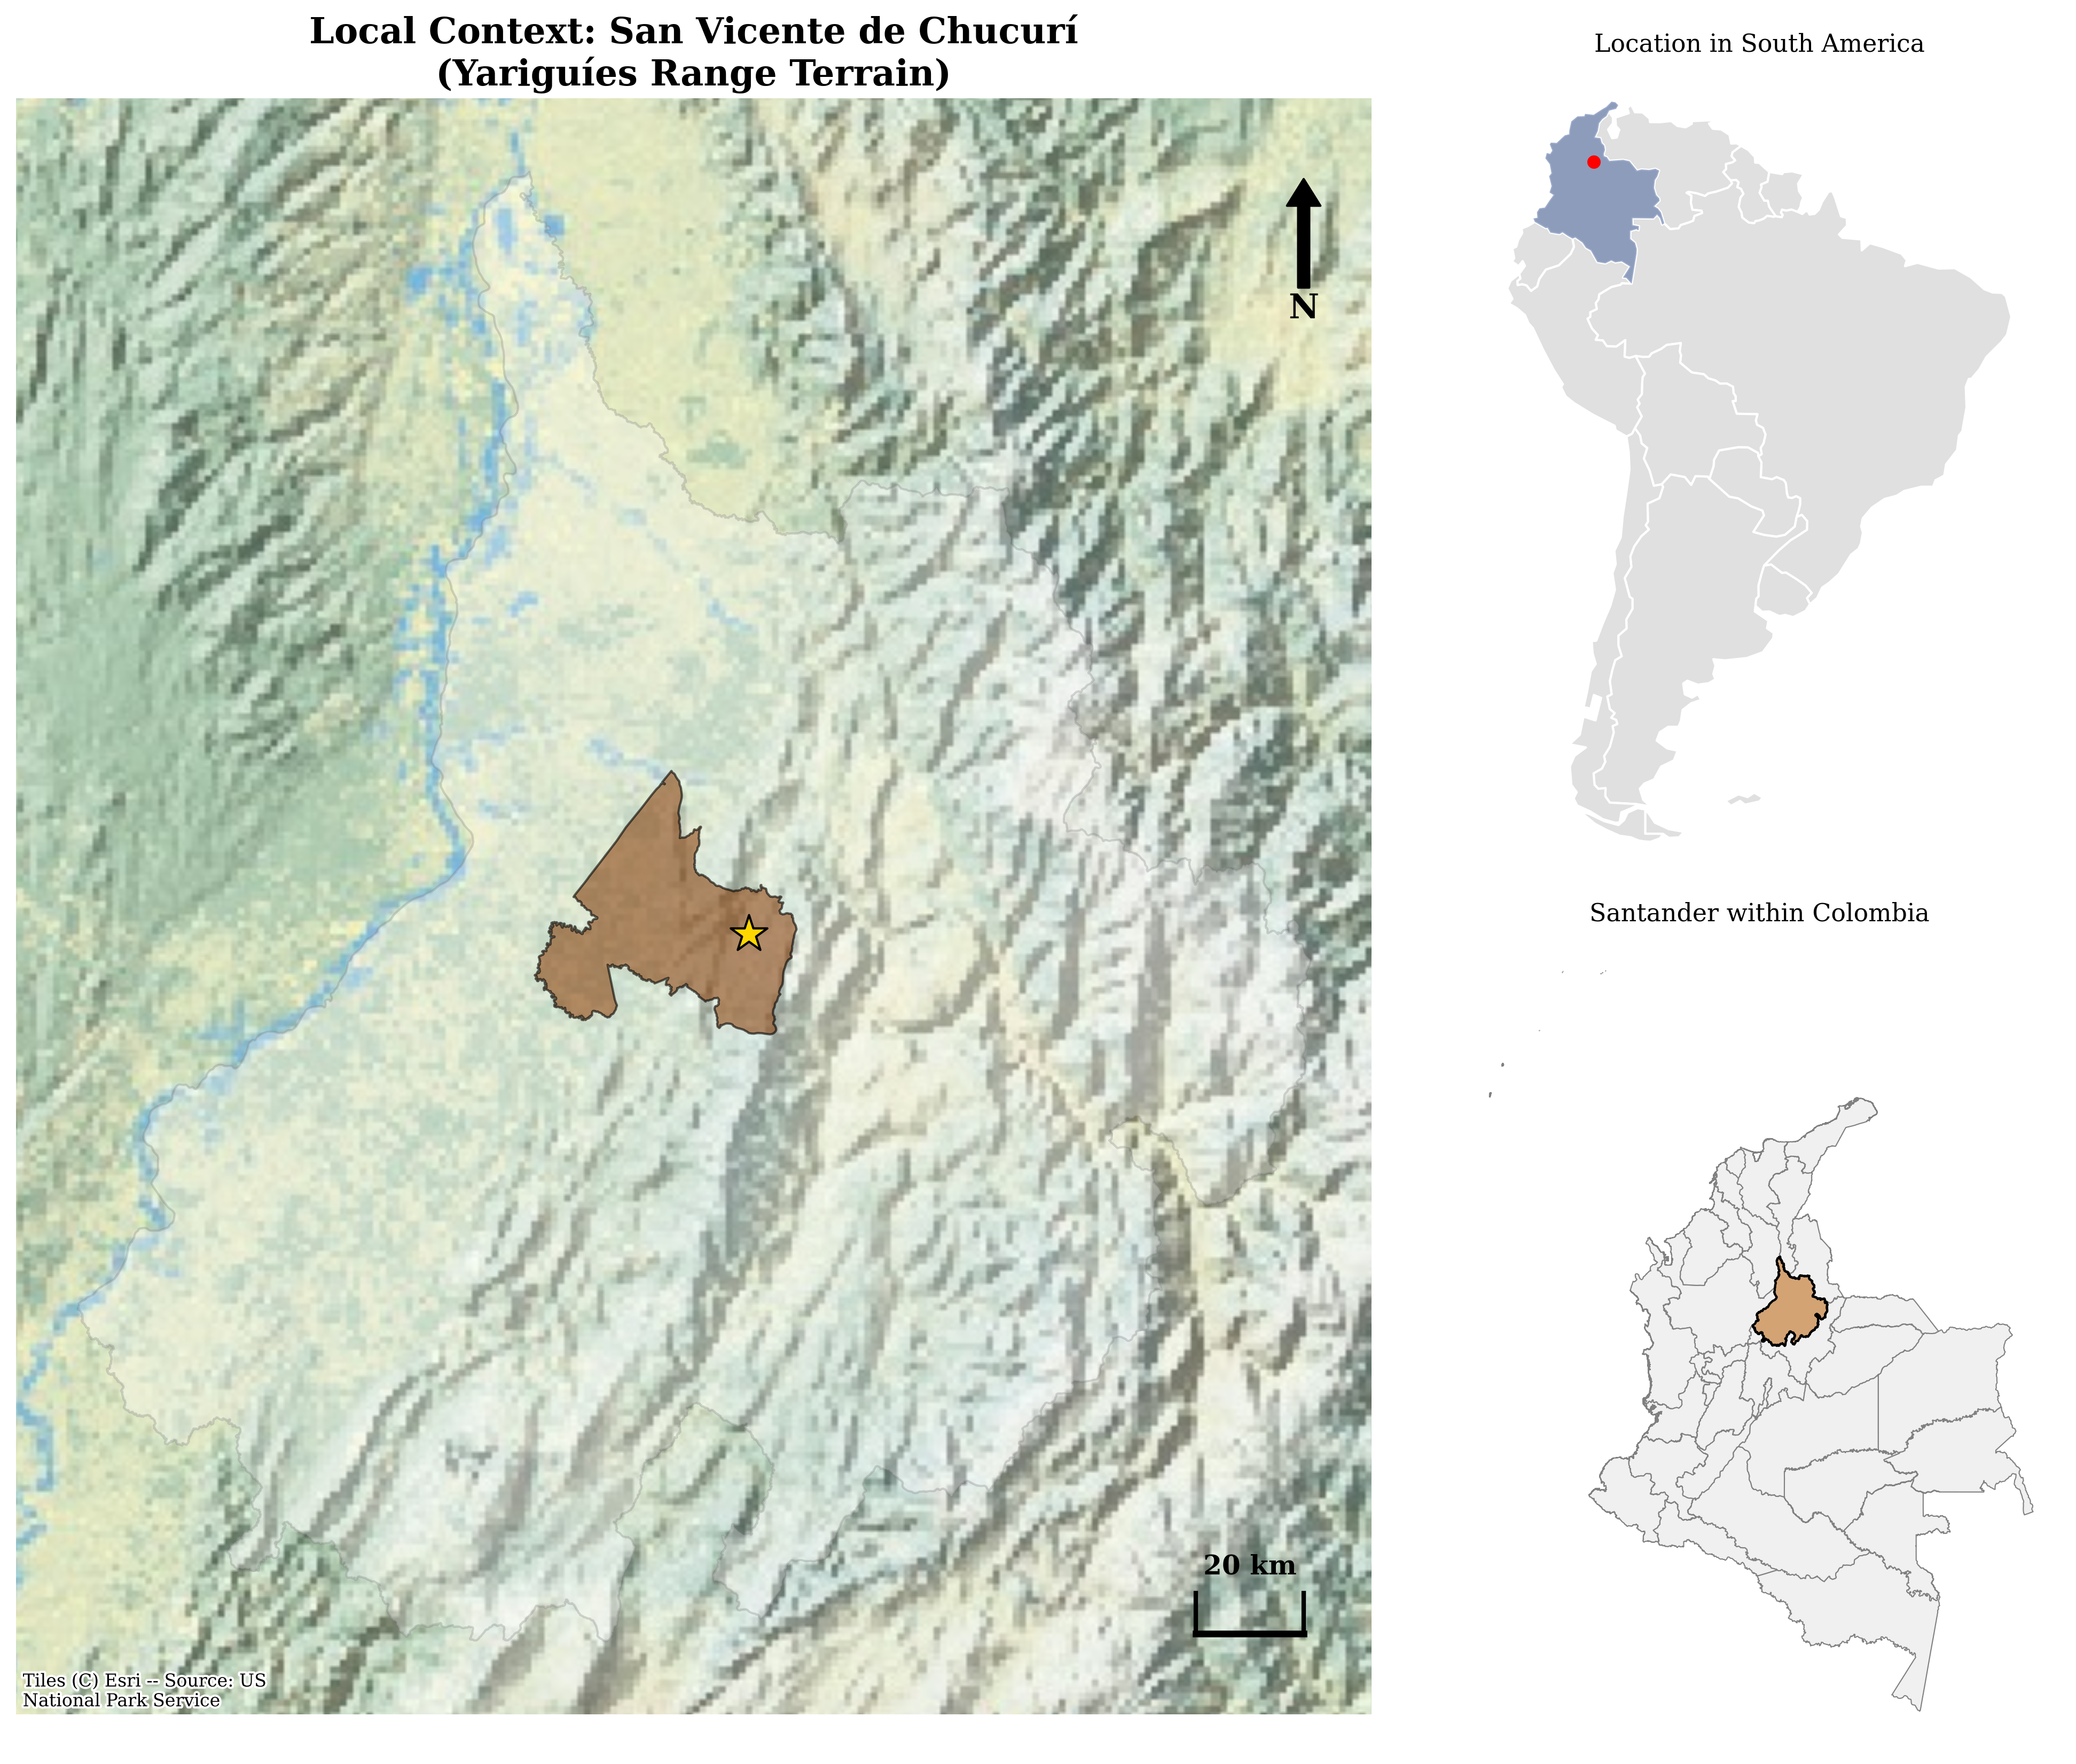
\includegraphics[width=0.95\linewidth]{figures/fig0_san_vicente_chucuri_map.png}
    \caption{Geographical location of San Vicente de Chucurí in Santander, Colombia. The map situates the municipality within the Colombian and South American contexts and highlights its location in the mountainous Yariguíes range, where cocoa-producing territories are shaped by rugged terrain, secondary-road access, and logistical sensitivity.}
    \label{fig:sanvicente}
\end{figure}


\subsection{Data Sources}

The integrated dataset combines four blocks. The first is the cocoa pricing chain: AgroNet weekly cacao reference prices aggregated to monthly Colombian producer-linked prices, the World Bank cocoa benchmark, and the Eurostat EU chocolate consumer price index. The second is a macro block composed of the COP/USD exchange rate and Brent oil prices, included because exchange-rate and energy movements help structure commodity-price transmission \citep{Jumah2001,JimenezRodriguez2022}. The third is a local weather block from NASA POWER for San Vicente de Chucuri, including precipitation, solar radiation, and temperature variables. The fourth is an official Santander disaster registry containing 594 event records from August 2021 to July 2024, including event categories, municipalities, and damage-related variables.

Figure~\ref{fig:coverage} shows the long-run coverage of the main price and macro series. The historical depth is uneven, which is why the article distinguishes clearly between long-run descriptive coverage and the much shorter aligned estimation windows.

\begin{figure}[H]
\centering
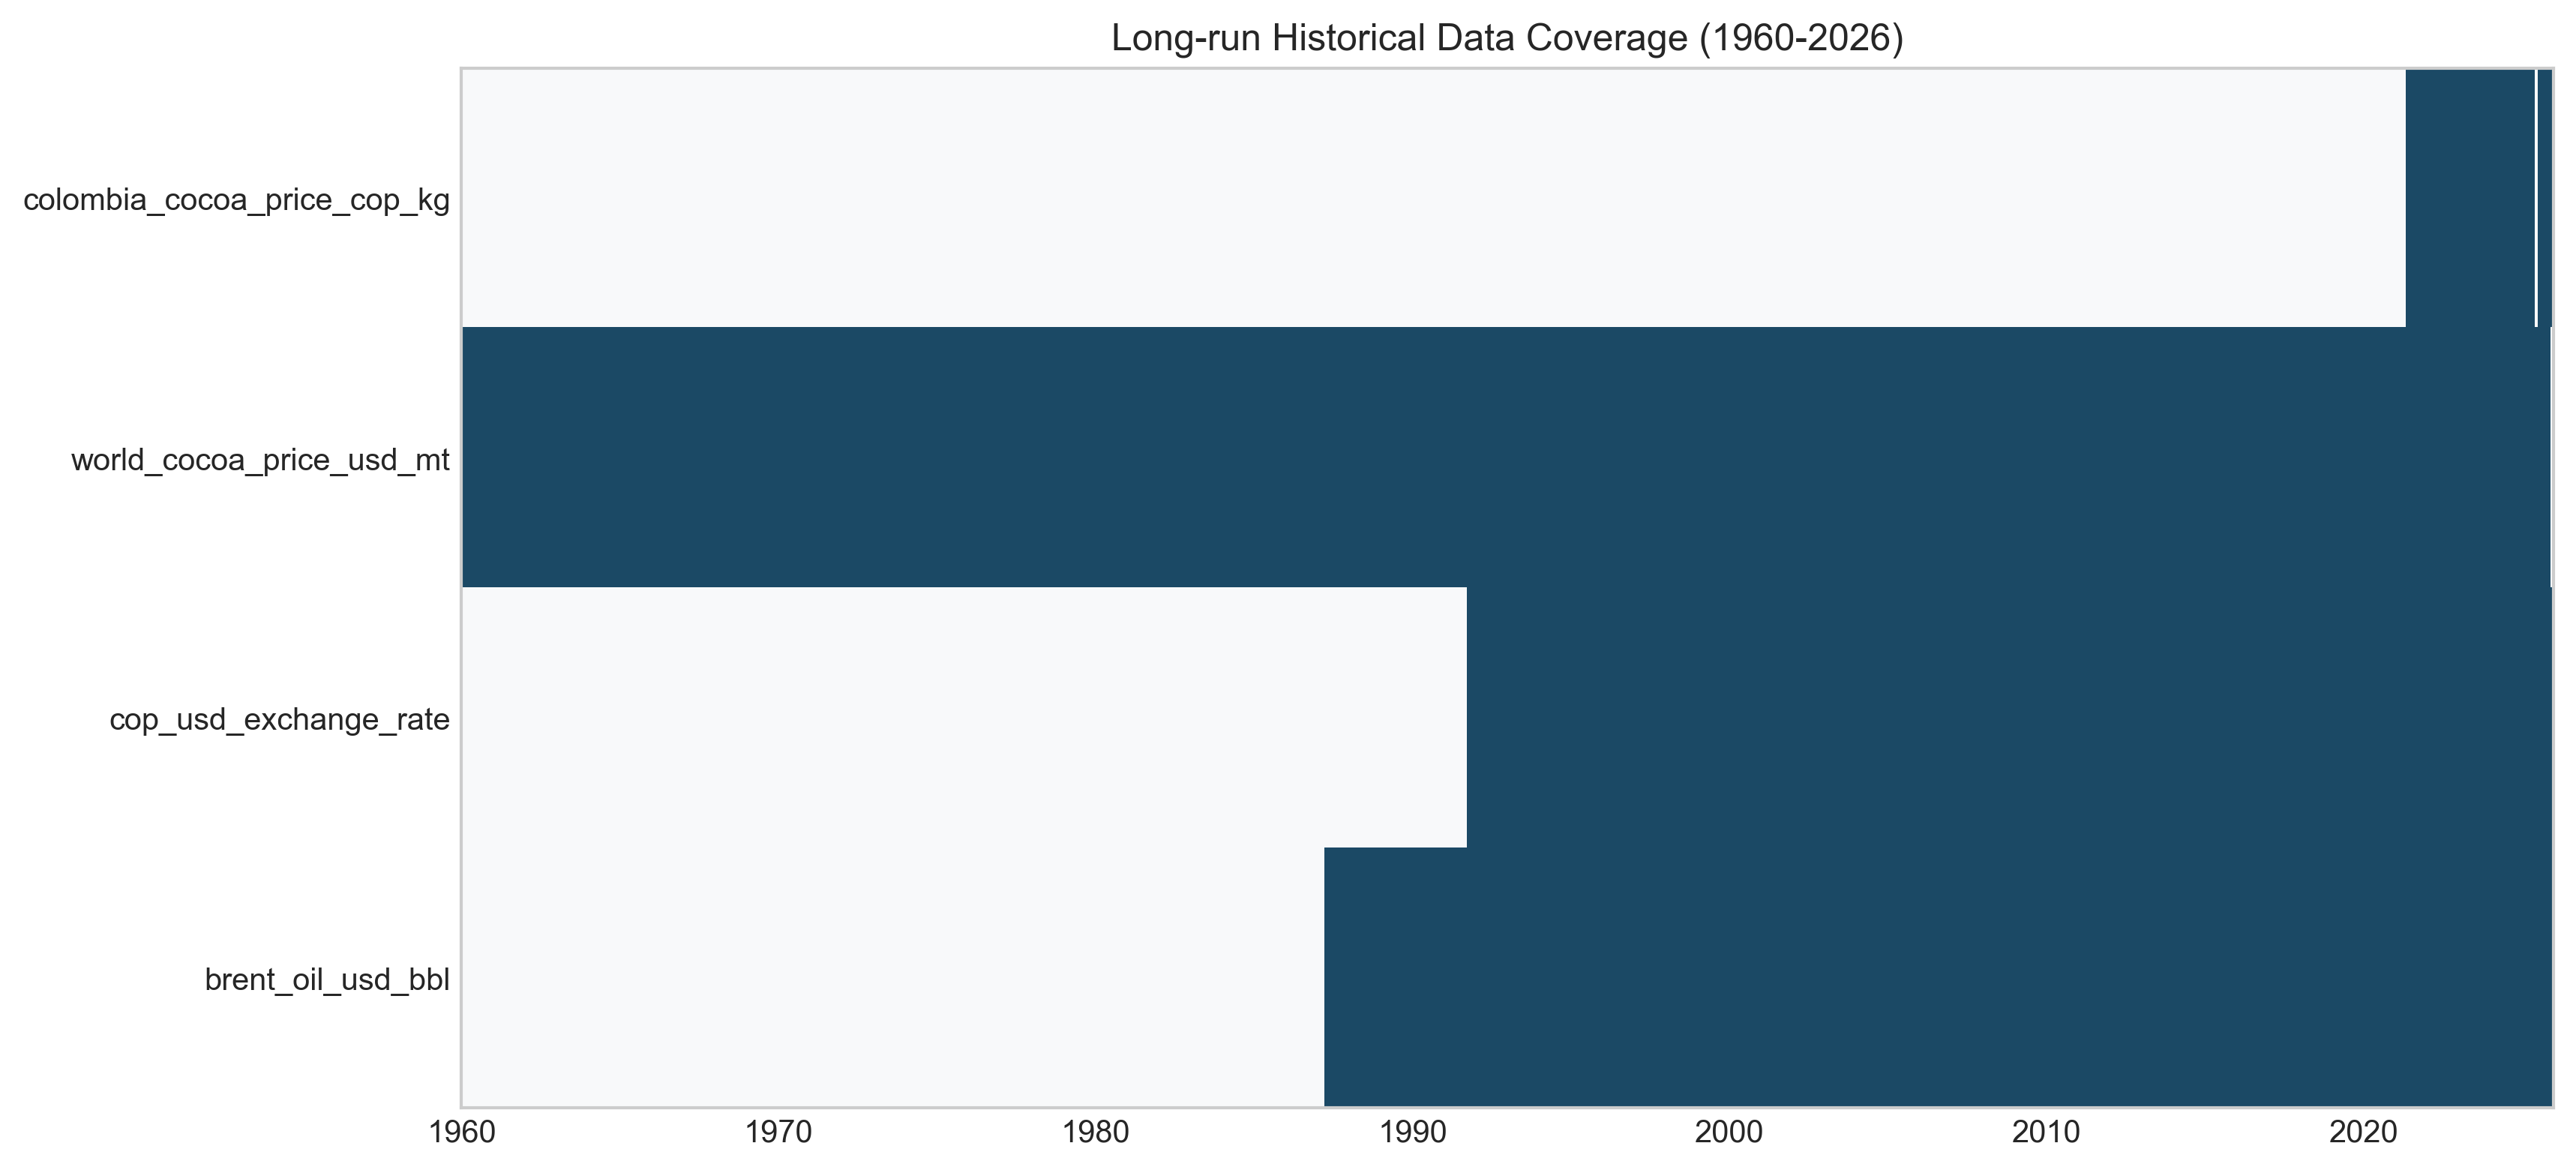
\includegraphics[width=0.9\textwidth]{figures/figure_v1_long_run_coverage.png}
\caption{Long-run historical coverage of the main price and macro series used in the integrated analysis. The figure highlights the difference between long repository coverage and the much shorter aligned estimation windows imposed by the Colombian domestic price series and the disaster registry.}
\label{fig:coverage}
\end{figure}

\subsection{Variable Card and Alignment}

Table~\ref{tab:data_card} summarizes the principal variables. The five core series define the transmission system. Weather variables and disaster indicators provide territorial stress information rather than replacing the benchmark system, and the disaster block is interpreted as a nested contextual layer rather than as a co-equal econometric price series.

\begin{table}[H]
\centering
\caption{Variable data card for the integrated analysis}
\label{tab:data_card}
\scriptsize
\setlength{\tabcolsep}{4pt}
\begin{tabular}{p{2.7cm}p{4.1cm}p{1.2cm}p{2.0cm}p{2.5cm}}
\toprule
Variable & Operational definition & Unit & Source & Usable window \\
\midrule
Colombian cocoa price & Monthly average of AgroNet weekly cacao reference prices & COP/kg & AgroNet & 2021-08 to 2026-03 \\
World cocoa benchmark & Monthly international cocoa price & USD/ton & World Bank & 1960-01 to 2026-02 \\
EU chocolate index & EU27 chocolate consumer price index & Index & Eurostat & 2016-12 to 2025-12 \\
COP/USD exchange rate & Monthly average peso-dollar exchange rate & COP/USD & BanRep & 1991-11 to 2026-03 \\
Brent oil price & Europe Brent monthly average spot price & USD/barrel & EIA & 1987-05 to 2026-03 \\
NASA precipitation & Monthly mean precipitation for San Vicente de Chucuri & mm/day & NASA POWER & 2000-01 to 2025-12 \\
NASA solar radiation & Monthly mean surface solar radiation & MJ/m$^2$/day & NASA POWER & 2000-01 to 2025-12 \\
NASA max temperature & Monthly mean maximum air temperature & $^\circ$C & NASA POWER & 2000-01 to 2025-12 \\
Hydrometeorological events & Monthly count of registry-coded hydrometeorological events & Count & Disaster registry & 2021-08 to 2024-07 \\
PCA disaster pressure & First principal component of monthly multi-hazard disruption features & Std. index & Disaster registry & 2021-08 to 2024-07 \\
\bottomrule
\end{tabular}
\end{table}

Table~\ref{tab:sample_design} reports the aligned windows used in the article. The full merged panel contains 795 monthly observations from January 1960 to March 2026, but direct comparative estimation is constrained by the overlap of the Colombian domestic series, the Eurostat downstream series, and the disaster registry. One domestic cocoa observation in September 2025 and one solar-radiation observation in December 2025 are completed through block-specific iterative imputation for continuity-sensitive figures. Those imputations do not create longer spans of observed data and are treated as transparent continuity devices rather than substitutes for additional information \citep{vanbuuren_groothuisoudshoorn_2011,troyanskaya_etal_2001}. The disaster registry is aggregated at the departmental level, the weather series are point-based for San Vicente de Chucuri, and the cocoa price series is a broader producer-linked reference. This scale mismatch is acceptable for contextual resilience analysis, but it cautions against reading the disaster layer as a precise local price-setting series.

\begin{table}[H]
\centering
\caption{Sample design and aligned estimation windows}
\label{tab:sample_design}
\small
\setlength{\tabcolsep}{4pt}
\begin{tabular}{p{5.1cm}p{1.7cm}p{3.2cm}p{4.0cm}}
\toprule
Panel or artifact & Obs. & Date span & Role in the article \\
\midrule
Full merged monthly panel & 795 & 1960-01 to 2026-03 & Long-run descriptive context \\
Core aligned levels window & 53 & 2021-08 to 2025-12 & Main levels comparisons and figures \\
Core aligned return window & 52 & 2021-09 to 2025-12 & Main short-run transmission models \\
Weather-augmented complete sample & 51 & 2021-08 to 2025-12 & Contextual weather extension \\
Nested disaster levels window & 36 & 2021-08 to 2024-07 & Disaster descriptives and registry aggregation \\
Nested disaster return window & 35 & 2021-09 to 2024-07 & Direct hazard and event-window models \\
\bottomrule
\end{tabular}
\end{table}

\section{Methodology}
\label{sec:methods}

\subsection{Transformations, Volatility, and Diagnostic Sequence}

For every strictly positive price series $P_{i,t}$, the main short-run object of interest is the log return
\begin{equation}
r_{i,t} = \Delta \ln(P_{i,t}) = \ln(P_{i,t}) - \ln(P_{i,t-1}),
\label{eq:logreturn}
\end{equation}
which expresses the proportional monthly shock transmitted through the chain. This transformation is appropriate both statistically and substantively. It improves comparability across variables measured in different units, reduces the dominance of level scale differences, and maps directly onto the paper's concern with shock transmission and instability rather than with raw nominal changes alone.

To characterize instability rather than average movement alone, the paper also uses a rolling volatility proxy based on the 12-month rolling standard deviation of returns:
\begin{equation}
\sigma_{i,t}^{(12)} =
\sqrt{\frac{1}{m_t - 1}\sum_{j=0}^{m_t-1}\left(r_{i,t-j}-\bar r_{i,t}^{(12)}\right)^2},
\label{eq:rolling_volatility}
\end{equation}
where $m_t$ is the number of non-missing returns available inside the rolling window up to month $t$. Stationarity diagnostics rely primarily on ADF tests in levels and returns, supplemented by ARCH-LM checks for volatility clustering. Given the short aligned span, these diagnostics are used to guide specification choice rather than to justify over-parameterized long-run systems \citep{hakkio_rush_1991}.

\subsection{Core Transmission Models}

The baseline levels association for the producer-linked Colombian price is
\begin{equation}
\ln(P^{COL}_{t}) = \alpha_0 + \alpha_1 \ln(P^{WLD}_{t}) + \alpha_2 \ln(FX_t) + \alpha_3 \ln(OIL_t) + u_t,
\label{eq:core_levels}
\end{equation}
where $P^{COL}_{t}$ is the Colombian cocoa price, $P^{WLD}_{t}$ the world cocoa benchmark, $FX_t$ the COP/USD exchange rate, and $OIL_t$ the Brent oil price. The short-run transmission model is
\begin{equation}
r^{COL}_{t} = \beta_0 + \beta_1 r^{WLD}_{t} + \beta_2 r^{FX}_{t} + \beta_3 r^{OIL}_{t} + \varepsilon_t.
\label{eq:core_returns}
\end{equation}
An analogous pair of models is estimated for the downstream EU chocolate index. All regressions are estimated with HAC-robust standard errors to account for heteroskedasticity and serial correlation in monthly data.

The levels equations provide a compact description of long-run co-movement in the short aligned span, but the paper does not treat them as proof of fully identified long-run equilibrium. For that reason, pairwise Engle-Granger and Granger-causality diagnostics are reported only as complementary evidence and are interpreted cautiously as reduced-form diagnostics rather than as strong structural claims.

\subsection{Structural Breaks, Tipping Points, and Regime-Sensitive Transmission}

To formalize the reviewer concern about tipping points and regime shifts, the core return-transmission equation is supplemented with a diagnostic structural-break layer inspired by the multiple-break logic of \citet{BaiPerron1998} and \citet{BaiPerron2003}. The diagnostic asks whether the relationship between Colombian cocoa returns and the world benchmark, exchange rate, and oil returns is better described by a single coefficient vector or by segment-specific coefficient vectors:
\begin{equation}
r^{COL}_{t} = \beta_{0,j} + \beta_{1,j}r^{WLD}_{t} + \beta_{2,j}r^{FX}_{t} + \beta_{3,j}r^{OIL}_{t} + e_t,
\quad t=T_{j-1}+1,\ldots,T_j .
\label{eq:break_returns}
\end{equation}
Because the aligned monthly return sample is short, the implementation is deliberately conservative. The script searches over feasible one-break partitions using segment-specific OLS residual sums of squares, imposes a minimum segment length of 18 monthly observations, and compares the no-break and one-break candidates using BIC. Segment-specific coefficients are reported only as diagnostic quantities. Candidate break dates are therefore interpreted as regime-sensitivity checks, not as causal evidence that disasters, weather anomalies, or policy changes generated a structural transition in prices. This layer is used to discipline the tipping-point language: if the data do not support a break under the conservative criterion, the manuscript retains the benchmark specification and treats threshold dynamics as a methodological concern for longer samples.

\subsection{Weather-Based Contextual Stress}

The weather block is used to represent local natural-capital stress without forcing the entire climate system into the core transmission specification. Following the project's prior variable-selection logic and local cocoa relevance, the weather-stress index is built from precipitation, surface solar radiation, and maximum temperature:
\begin{equation}
\mathrm{WeatherStress}_t =
\frac{1}{J}\sum_{j=1}^{J}\left|z(w_{j,t})\right|,
\label{eq:weather_stress}
\end{equation}
where $w_{j,t}$ denotes the selected weather variable and $z(\cdot)$ its within-sample standardization. The resulting index is interpreted as a contextual anomaly score and a threshold-relevant indicator, not as a measured farm-level physiological threshold. Precipitation anomalies proxy soil-moisture stress, flooding pressure, disease conditions, and harvest logistics; solar-radiation anomalies proxy shade, evapotranspiration, and disease-pressure context; and maximum-temperature anomalies proxy heat exposure relevant to flowering, pod development, and labor conditions. In this sense, the NASA POWER variables serve as natural-capital stress proxies for conditions that may move the cocoa system closer to physiological or logistical tipping points. Weather-extended domestic models are estimated as a parsimonious sensitivity exercise in which lagged standardized weather covariates are added to Equation~\ref{eq:core_returns}. Their role is diagnostic: they show whether local environmental stress materially changes the transmission estimates or mainly sharpens the vulnerability interpretation.

\subsection{Contextual Disaster Exposure Layer}

The disaster registry is not modeled as a second transmission system. Four features rule out that interpretation. First, the disaster window is shorter than the core return window. Second, registry-based hazard counts are sparse, irregular, and sometimes strongly zero-inflated. Third, the composite disaster indicator pools heterogeneous event, damage, and spread variables into a synthetic territorial-pressure construct. Fourth, the registry is aggregated at a different spatial scale from both the point-based weather series and the broader producer-linked price series. For these reasons, the disaster layer is used only as a contextual exposure block through descriptive overlays, a parsimonious one-at-a-time hazard screen, and an exploratory event-window comparison, rather than being forced into a large joint VAR/VECM with the benchmark system \citep{hakkio_rush_1991,lutkepohl_2005,acosta_ihle_voncramon_2019,Parsons2021,Garschagen2021}.

The disaster registry is handled in two stages. First, candidate direct hazard series are screened within the nested disaster return window. The screening focuses on monthly variation, the number of non-zero months, and conceptual interpretability. Isolated earthquake counts are assessed explicitly because they were the original candidate hazard series in the second manuscript version, but they are too sparse for direct time-series use. Hydrometeorological counts, geophysical counts, and total monthly event counts are then evaluated as alternative contextual signals. The objective is not to identify a co-equal price driver, but to determine whether any registry-based monthly count is dense enough to serve as a parsimonious territorial episode marker.

The selected direct hazard overlay uses standardized hydrometeorological counts $H_t$:
\begin{equation}
r^{COL}_{t} = \gamma_0 + \gamma_1 r^{WLD}_{t} + \gamma_2 r^{FX}_{t} + \gamma_3 r^{OIL}_{t} + \gamma_4 H_t + \nu_t,
\label{eq:hazard_return_overlay}
\end{equation}
while the corresponding volatility specification is
\begin{equation}
\sigma^{COL}_{t} = \delta_0 + \delta_1 \sigma^{WLD}_{t} + \delta_2 H_t + \upsilon_t.
\label{eq:hazard_vol_overlay}
\end{equation}
These models are intentionally modest. They test whether a direct monthly hazard count adds information once the benchmark transmission channel is already controlled for. Even in this specification, $H_t$ is interpreted as an exposure marker appended to the core model, not as a benchmark-like driver with an autonomous transmission role.

Second, a synthetic multi-hazard robustness overlay is constructed using principal component analysis on 21 eligible standardized monthly disaster features, including event frequency, municipal spread, human impact, housing damage, and infrastructure damage:
\begin{equation}
D_t = \sum_{k=1}^{K} w_k z(F_{k,t}).
\label{eq:pca_indicator}
\end{equation}
This PCA indicator is not treated as the primary result when a direct hazard series is feasible. Instead, it functions as a robustness layer that summarizes broader multi-hazard pressure and helps identify whether the direct hazard peak is also visible in the composite registry structure. Loadings, variable blocks, variance explained, and peak months are reported as transparency diagnostics. In line with the composite-indicator literature, $D_t$ is interpreted as a synthetic territorial-pressure construct rather than as a canonical economic time series or direct causal price driver \citep{Parsons2021,Garschagen2021}.

\subsection{Event-Based Mean-Shift Design}

Because disaster exposure may appear as discrete stress episodes rather than stable linear coefficients, the analysis also implements a simple episode-window comparison around the peak hazard month $t^{*}$:
\begin{equation}
r^{COL}_{t} = \theta_0 + \theta_1 \mathbf{1}(t \ge t^{*}) + e_t,
\label{eq:event_shift}
\end{equation}
evaluated in symmetric six-month windows before and after the identified peak. In practice, the main inference is based on Welch, Levene, and Kolmogorov-Smirnov comparisons across the pre- and post-peak windows. The peak month is selected from the hazard screen itself, which makes the event window exploratory and data-driven rather than an externally imposed quasi-experiment. This event-based design is used because the short disaster overlap is more compatible with transparent episode stratification than with an overextended dynamic hazard system. The resulting comparison informs the resilience-dividend discussion only cautiously: it identifies a period in which benchmark exposure and territorial pressure coincide, but it does not test whether agroforestry, diversified livelihoods, or any other buffer capacity caused lower volatility.

\section{Results}
\label{sec:results}

\subsection{Descriptive Structure and Statistical Properties}

The aligned sample already shows why the paper separates the benchmark system from the environmental block. Table~\ref{tab:descriptive_stats} reports the levels and dispersion of the main series in the aligned window. Colombian and world cocoa prices are far more volatile than the EU downstream chocolate index, while the local weather series display distinct seasonal and anomaly structures rather than simple co-trending price behavior.

\begin{table}[H]
\centering
\caption{Descriptive statistics for the core system and selected weather variables in the aligned window}
\label{tab:descriptive_stats}
\small
\begin{tabular}{p{4.0cm}rrrrr}
\toprule
Series & Mean & Std. dev. & Median & Min & Max \\
\midrule
Colombian cocoa price & 17{,}334.75 & 9{,}168.37 & 12{,}536.69 & 7{,}926.08 & 34{,}395.33 \\
World cocoa benchmark & 4{,}943.44 & 2{,}660.61 & 3{,}630.14 & 2{,}239.13 & 10{,}745.11 \\
EU chocolate index & 128.83 & 19.73 & 125.20 & 104.25 & 164.99 \\
COP/USD exchange rate & 4{,}147.16 & 302.33 & 4{,}047.41 & 3{,}773.38 & 4{,}926.66 \\
Brent oil price & 82.61 & 13.41 & 80.92 & 62.54 & 122.71 \\
NASA precipitation & 5.73 & 3.59 & 5.08 & 0.03 & 14.67 \\
NASA max temperature & 31.93 & 3.04 & 30.79 & 28.67 & 39.15 \\
NASA solar radiation & 18.24 & 1.19 & 18.18 & 15.68 & 20.62 \\
\bottomrule
\end{tabular}
\end{table}

Table~\ref{tab:stats_overview} shows that the core price series behave as non-stationary processes in levels over the aligned window, whereas return transformations are much more stable. Several weather series reject the ADF unit-root null already in levels, which reinforces the decision to treat environmental stress as a contextual block rather than to force the whole system into one long-run specification.

\begin{table}[H]
\centering
\caption{Selected statistical properties from the aligned panel}
\label{tab:stats_overview}
\resizebox{\textwidth}{!}{%
\begin{tabular}{p{4.2cm}rrrrr}
\toprule
Series & Mean level & Annualized vol. & ADF level $p$ & ADF return $p$ & ARCH-LM $p$ \\
\midrule
Colombian cocoa price & 17{,}334.75 & 0.376 & 0.643 & 0.000 & 0.768 \\
World cocoa benchmark & 4{,}943.44 & 0.367 & 0.648 & 0.000 & 0.013 \\
EU chocolate index & 128.83 & 0.030 & 0.984 & 0.013 & 0.005 \\
COP/USD exchange rate & 4{,}147.16 & 0.110 & 0.525 & 0.000 & 0.903 \\
Brent oil price & 82.61 & 0.258 & 0.460 & 0.081 & 0.083 \\
NASA precipitation & 5.73 & 3.106 & 0.000 & 0.006 & 0.070 \\
NASA max temperature & 31.93 & 0.152 & 0.018 & 0.003 & 0.438 \\
NASA solar radiation & 18.25 & 0.283 & 0.000 & 0.000 & 0.434 \\
\bottomrule
\end{tabular}
}
\end{table}

Figure~\ref{fig:indexed_core} illustrates the proportional co-movement that defines the core transmission problem. Colombian and world cocoa prices move closely through the 2024--2025 boom and correction, whereas the EU downstream index follows a much smoother path.

\begin{figure}[H]
\centering
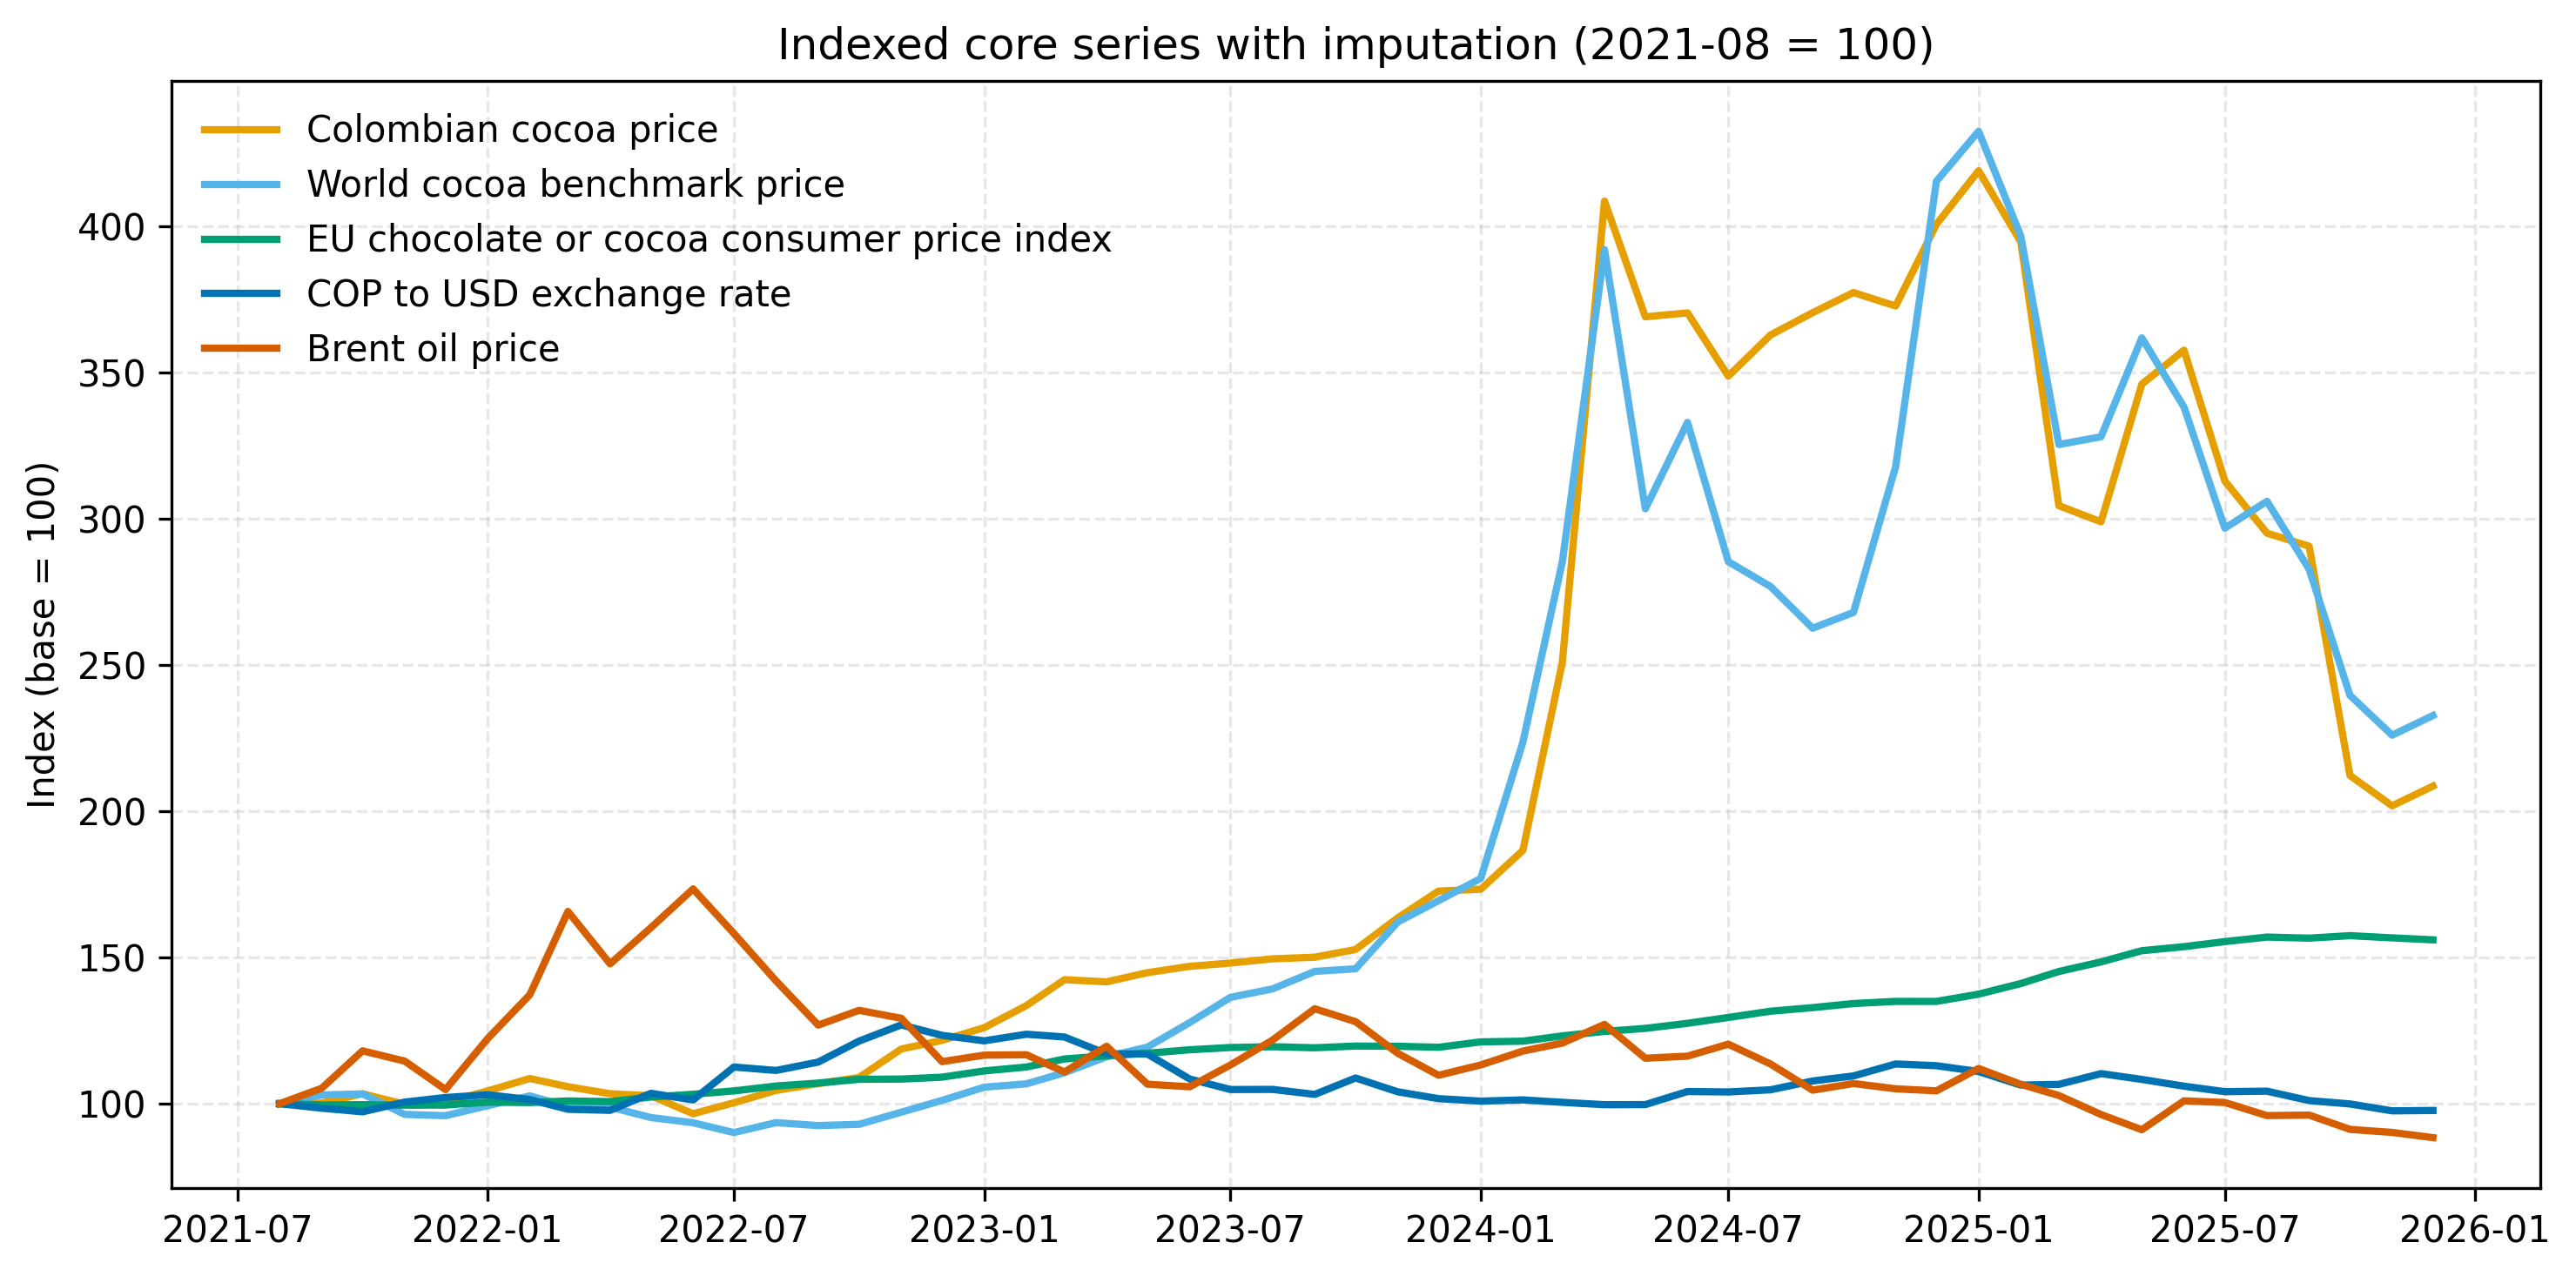
\includegraphics[width=0.95\textwidth]{figures/figure_indexed_core_series_common_window_imputed.png}
\caption{Indexed core series in the aligned monthly window (August 2021 = 100). The close co-movement between the Colombian and world cocoa series contrasts with the smoother adjustment of the downstream EU chocolate index.}
\label{fig:indexed_core}
\end{figure}

\subsection{Supply-Chain Transmission}

Table~\ref{tab:transmission_results} reports the main transmission elasticities. The central result is stable across the earlier manuscript versions and remains the strongest result in the integrated article: world cocoa returns are the dominant short-run driver of Colombian producer-linked returns. In the core return model, the world benchmark coefficient is 0.796 ($p<0.001$). The corresponding levels association is also close to one. By contrast, the downstream EU chocolate index has a weaker and slower link to the world benchmark. Its levels coefficient is positive, but the return specification has very low fit and a small negative short-run coefficient.

\begin{table}[H]
\centering
\caption{Domestic and downstream price transmission results}
\label{tab:transmission_results}
\small
\begin{tabular}{lrrrr}
\toprule
Model component & Coefficient & Std. error & $p$-value & Adj. $R^2$ \\
\midrule
\textit{Producer-linked domestic price} & & & & \\
$\ln(P^{COL}_{t}) \leftarrow \ln(P^{WLD}_{t})$ & 0.990 & 0.037 & $<0.001$ & 0.965 \\
$\ln(P^{COL}_{t}) \leftarrow \ln(FX_t)$ & 0.902 & 0.147 & $<0.001$ & 0.965 \\
$\Delta \ln(P^{COL}_{t}) \leftarrow \Delta \ln(P^{WLD}_{t})$ & 0.796 & 0.180 & $<0.001$ & 0.581 \\
$\Delta \ln(P^{COL}_{t}) \leftarrow \Delta \ln(FX_t)$ & 0.218 & 0.204 & 0.287 & 0.581 \\
\midrule
\textit{Downstream EU chocolate index} & & & & \\
$\ln(P^{EU}_{t}) \leftarrow \ln(P^{WLD}_{t})$ & 0.296 & 0.126 & 0.018 & 0.727 \\
$\Delta \ln(P^{EU}_{t}) \leftarrow \Delta \ln(P^{WLD}_{t})$ & -0.023 & 0.010 & 0.023 & -0.007 \\
\bottomrule
\end{tabular}
\end{table}

This pattern supports an uneven-adjustment interpretation. Producer-linked prices absorb benchmark volatility rapidly, while the downstream consumer layer appears more buffered. Pairwise Granger results, retained in the supplementary section, support predictive precedence from world to Colombian cocoa at lag 3 but also show reverse predictive links in the short sample. The appropriate conclusion is therefore reduced-form rather than structural: benchmark transmission is the clearest observable exposure mechanism, but the short aligned span does not warrant stronger claims about a fully identified dynamic chain.

\subsection{Structural-Break and Tipping-Point Diagnostics}

Table~\ref{tab:structural_breaks} reports the regime-sensitive diagnostic for the core return equation. The no-break model is retained by BIC. The best one-break candidate occurs in May 2024, splitting the 52-return sample into 32 and 20 observations, but its BIC is weaker than the no-break benchmark. The world-benchmark coefficient is larger before the candidate split and smaller afterward, but because the candidate is not selected, this difference is treated only as a sensitivity check. The result is useful precisely because it restrains the tipping-point language: the aligned monthly data do not justify claiming a detected transmission regime shift, even though the framework remains appropriate for longer samples and future monitoring.

\begin{table}[H]
\centering
\caption{Diagnostic structural-break screen for the core domestic return-transmission equation}
\label{tab:structural_breaks}
\small
\resizebox{\textwidth}{!}{%
\begin{tabular}{p{4.2cm}rrrrrrp{6.2cm}}
\toprule
Model & Break date & Segment before & Segment after & BIC criterion & World $\beta$ before & World $\beta$ after & Interpretation \\
\midrule
No-break benchmark & -- & 52 & 0 & -264.475 & 0.796 & -- & BIC-selected baseline for the core transmission model. \\
Best one-break candidate & 2024-05 & 32 & 20 & -258.141 & 1.126 & 0.588 & Not retained by BIC; diagnostic only, not a detected regime shift. \\
\bottomrule
\end{tabular}
}
\end{table}

\subsection{Environmental Stress, Hazards, and Resilience Overlay}

Environmental stress is present beyond the disaster registry. The weather-extended domestic models retained from the first manuscript version improve fit only modestly relative to the core transmission equations (increase in adjusted $R^2$ of 0.0017 in levels and 0.0139 in returns), and most individual weather coefficients remain statistically weak. That finding is substantively useful because it supports a contextual interpretation of local natural-capital stress rather than a claim that weather replaces benchmark transmission as the main short-run price mechanism. The weather-stress index averages absolute standardized anomalies in precipitation, solar radiation, and maximum temperature; across the aligned window its mean is 0.798 with a standard deviation of 0.356. Figure~\ref{fig:vulnerability} summarizes this full-window contextual layer through the weather-stress score and the exploratory exposure indices.

\begin{figure}[H]
\centering
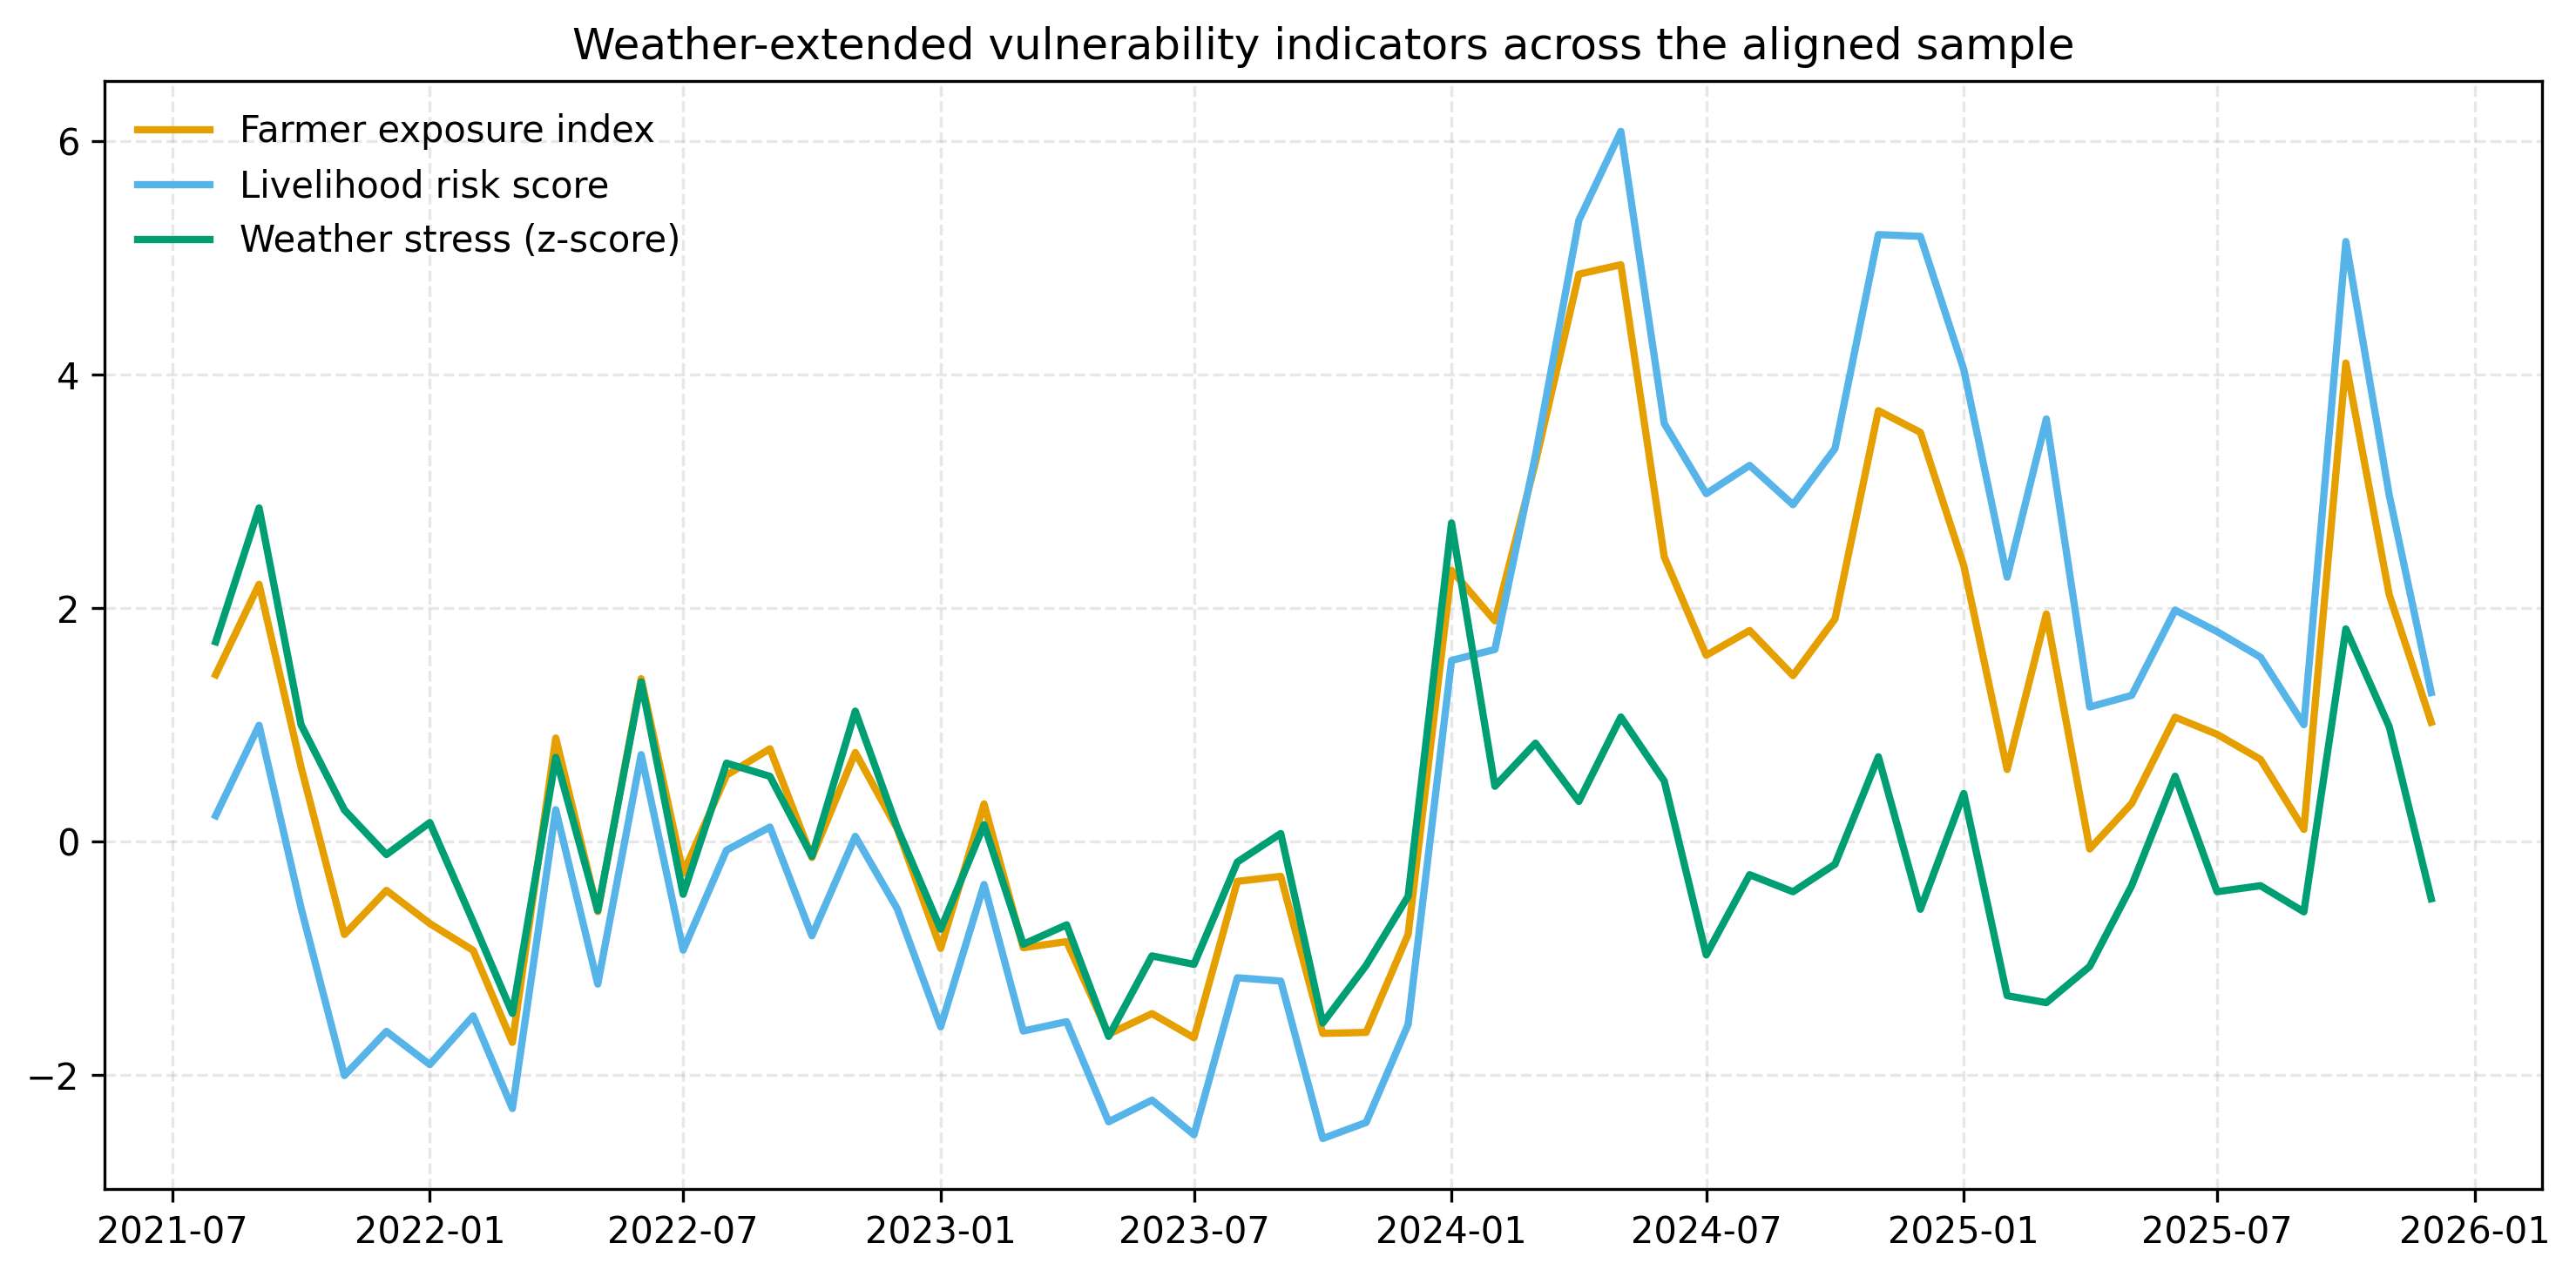
\includegraphics[width=0.93\textwidth]{figures/figure_weather_vulnerability_index.png}
\caption{Weather-extended contextual indicators across the aligned sample. The figure summarizes local weather anomalies together with benchmark-driven exposure and volatility proxies, showing when environmental stress and market instability accumulate in the same months.}
\label{fig:vulnerability}
\end{figure}

The nested disaster window sharpens that interpretation. Figure~\ref{fig:disaster_dynamics} shows the monthly event totals and hazard-domain mix for Santander. Hydrometeorological and geophysical events dominate the coded event structure, whereas isolated earthquakes are infrequent.

\begin{figure}[H]
\centering
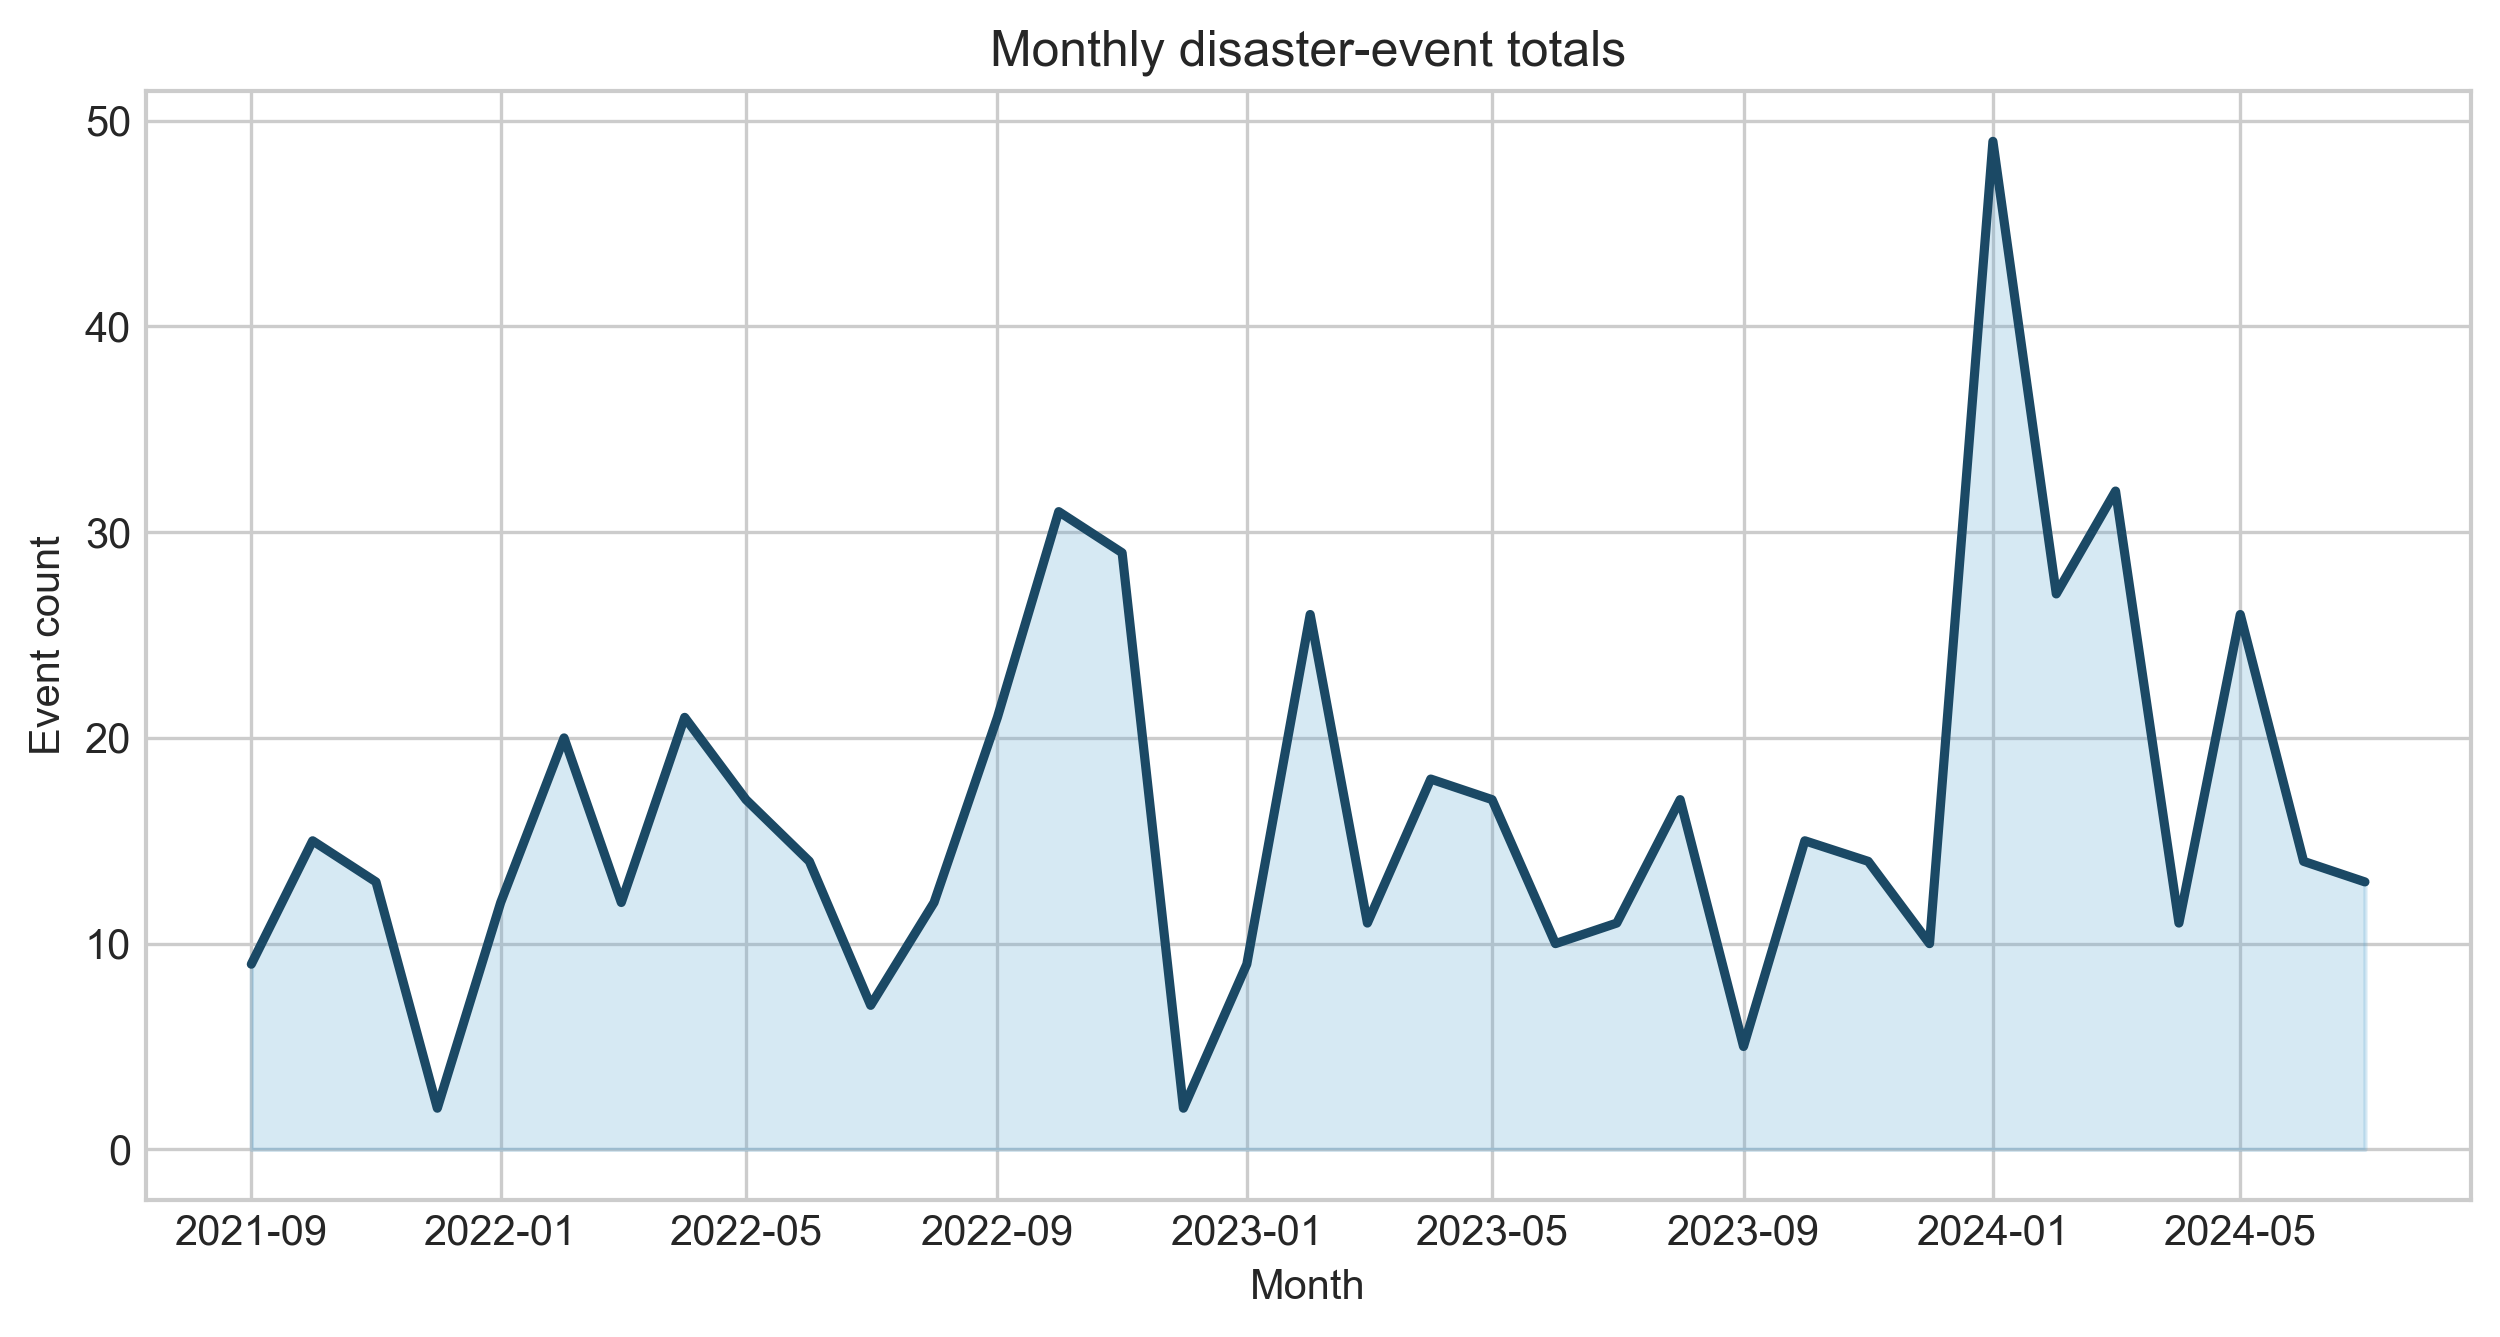
\includegraphics[width=0.48\textwidth]{figures/figure_monthly_event_totals.png}
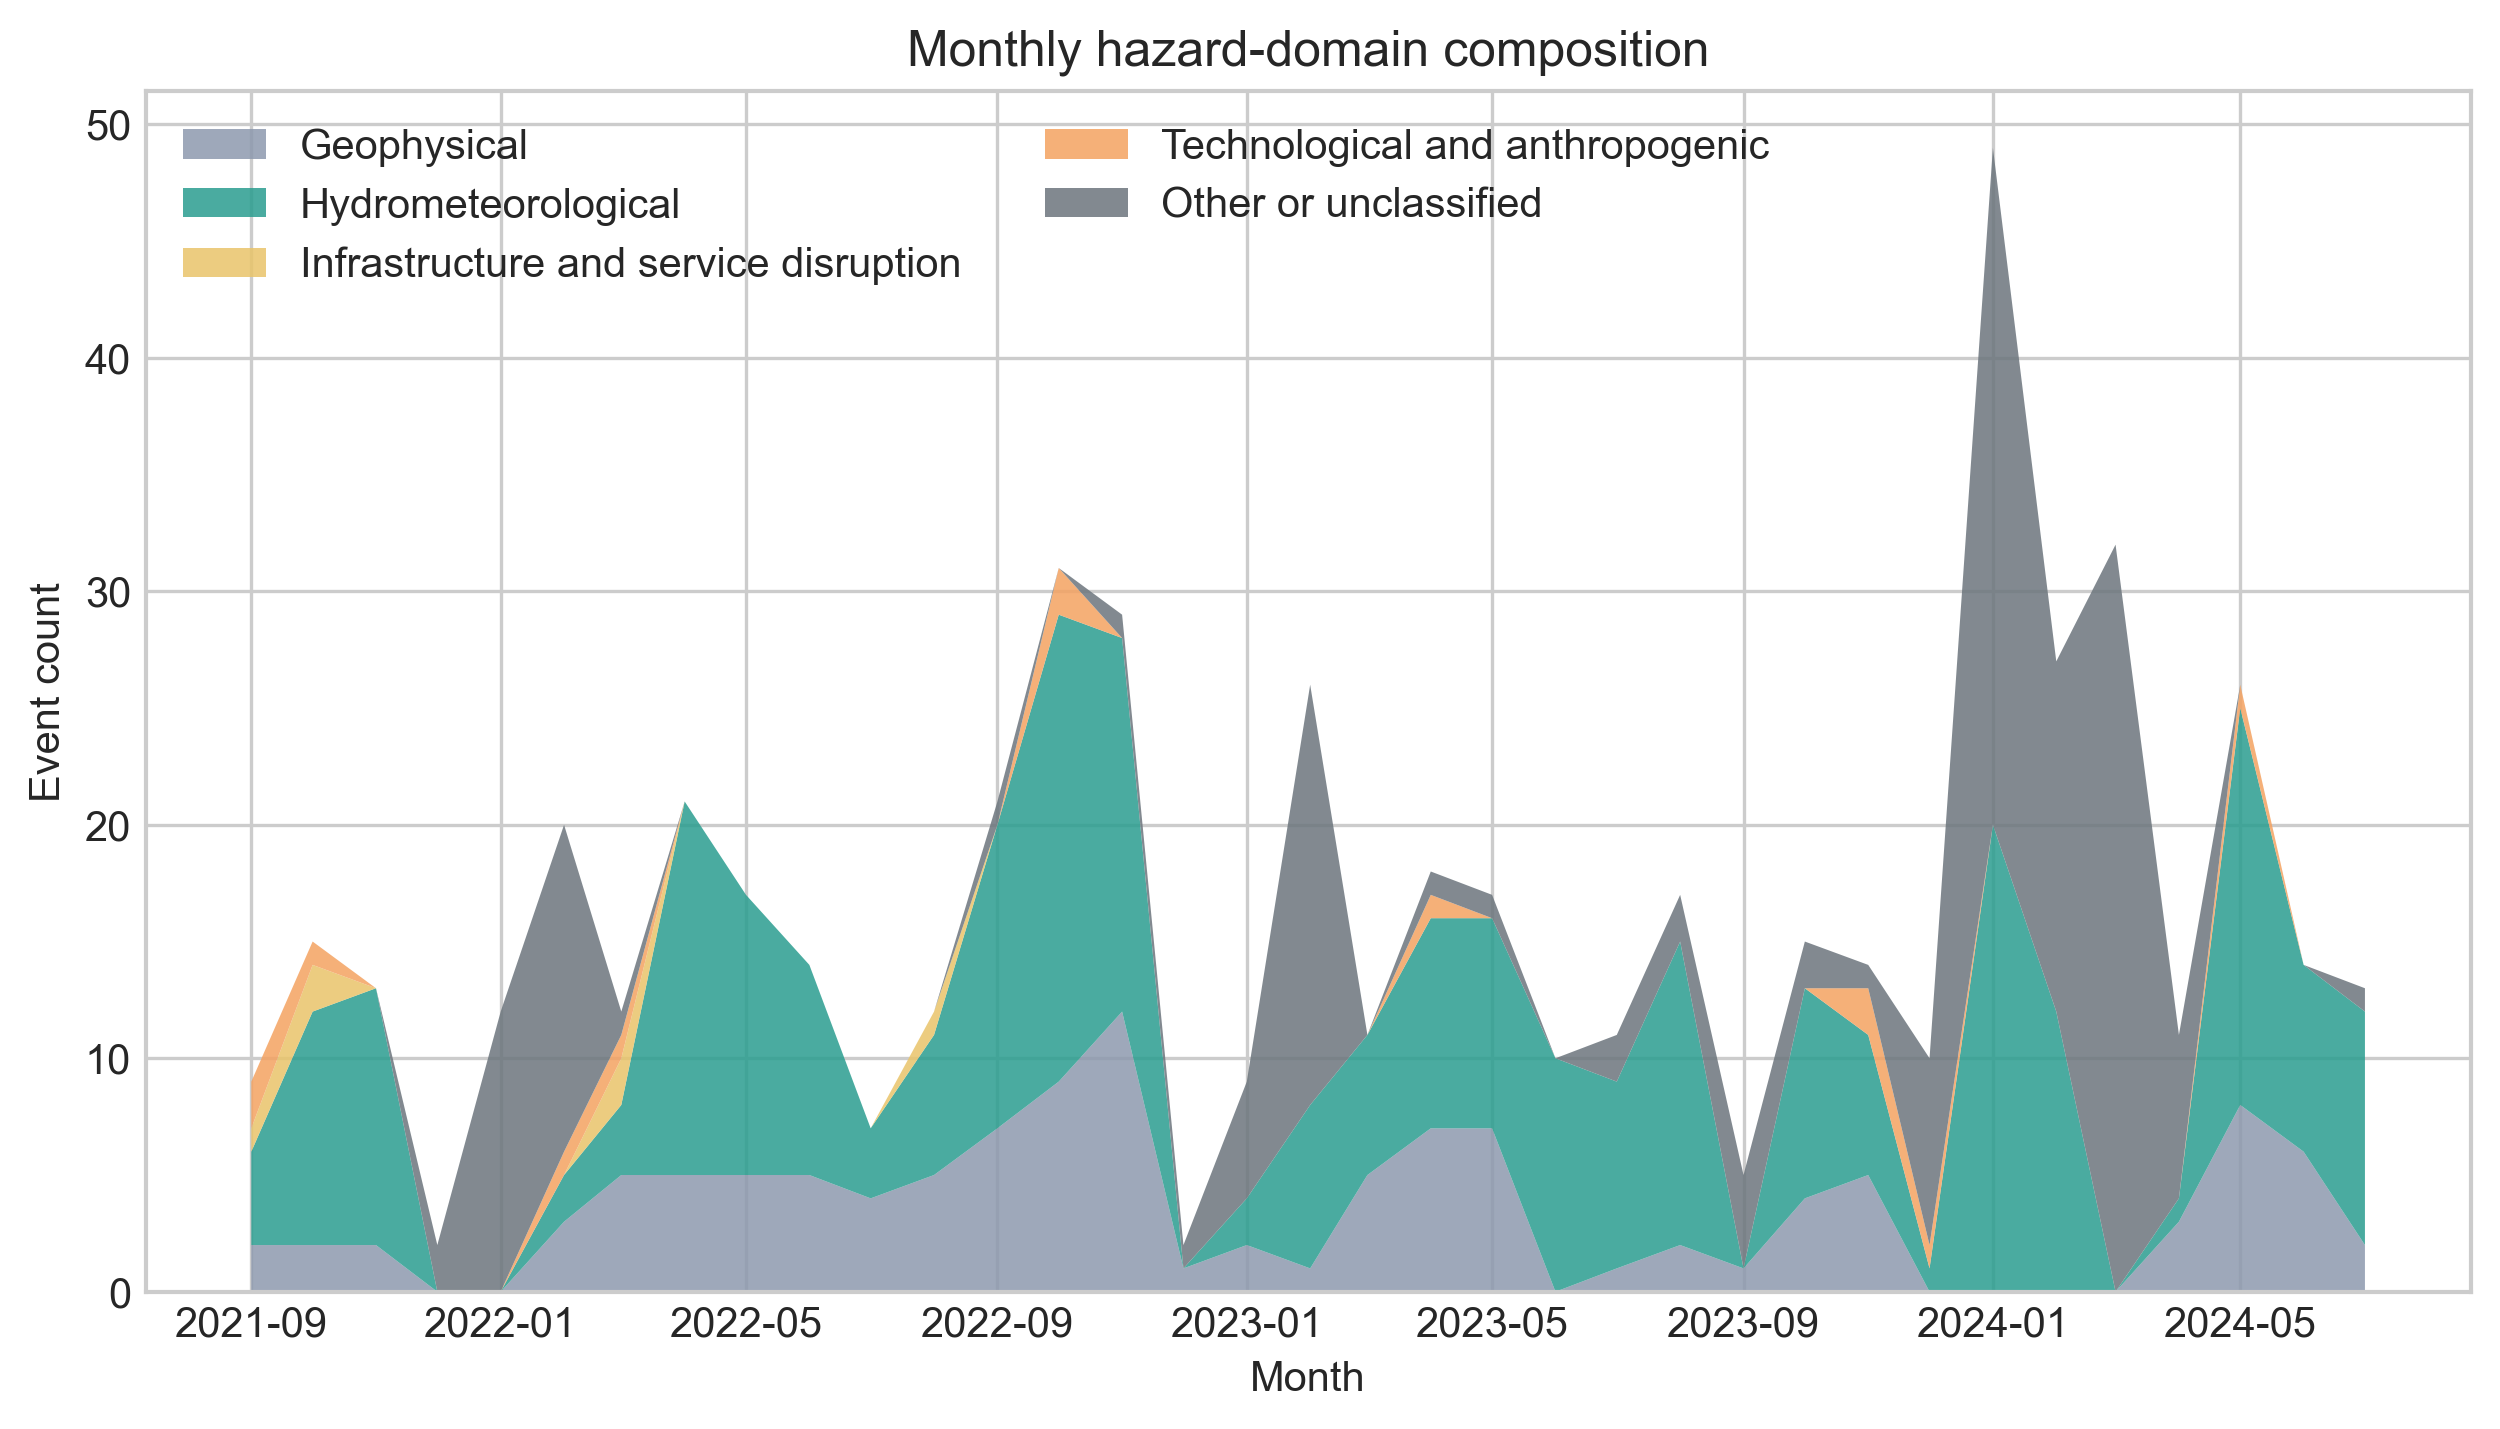
\includegraphics[width=0.48\textwidth]{figures/figure_hazard_domain_mix.png}
\caption{Disaster event dynamics and hazard-domain composition in Santander, August 2021--July 2024. Monthly totals reveal recurrent pressure rather than isolated single-shock episodes, and the hazard mix is dominated by hydrometeorological and geophysical events.}
\label{fig:disaster_dynamics}
\end{figure}

Figure~\ref{fig:contextual_alignment} aligns the world and Colombian cocoa returns with the hydrometeorological count and the composite territorial-pressure index in the nested window. The contrast in signal shape is central to the paper's revised methodology. The benchmark series move as continuous market returns, whereas the disaster series behave as episodic and uneven territorial signals. Their value lies in identifying months of intensified local pressure, not in behaving like a second benchmark.

\begin{figure}[H]
\centering
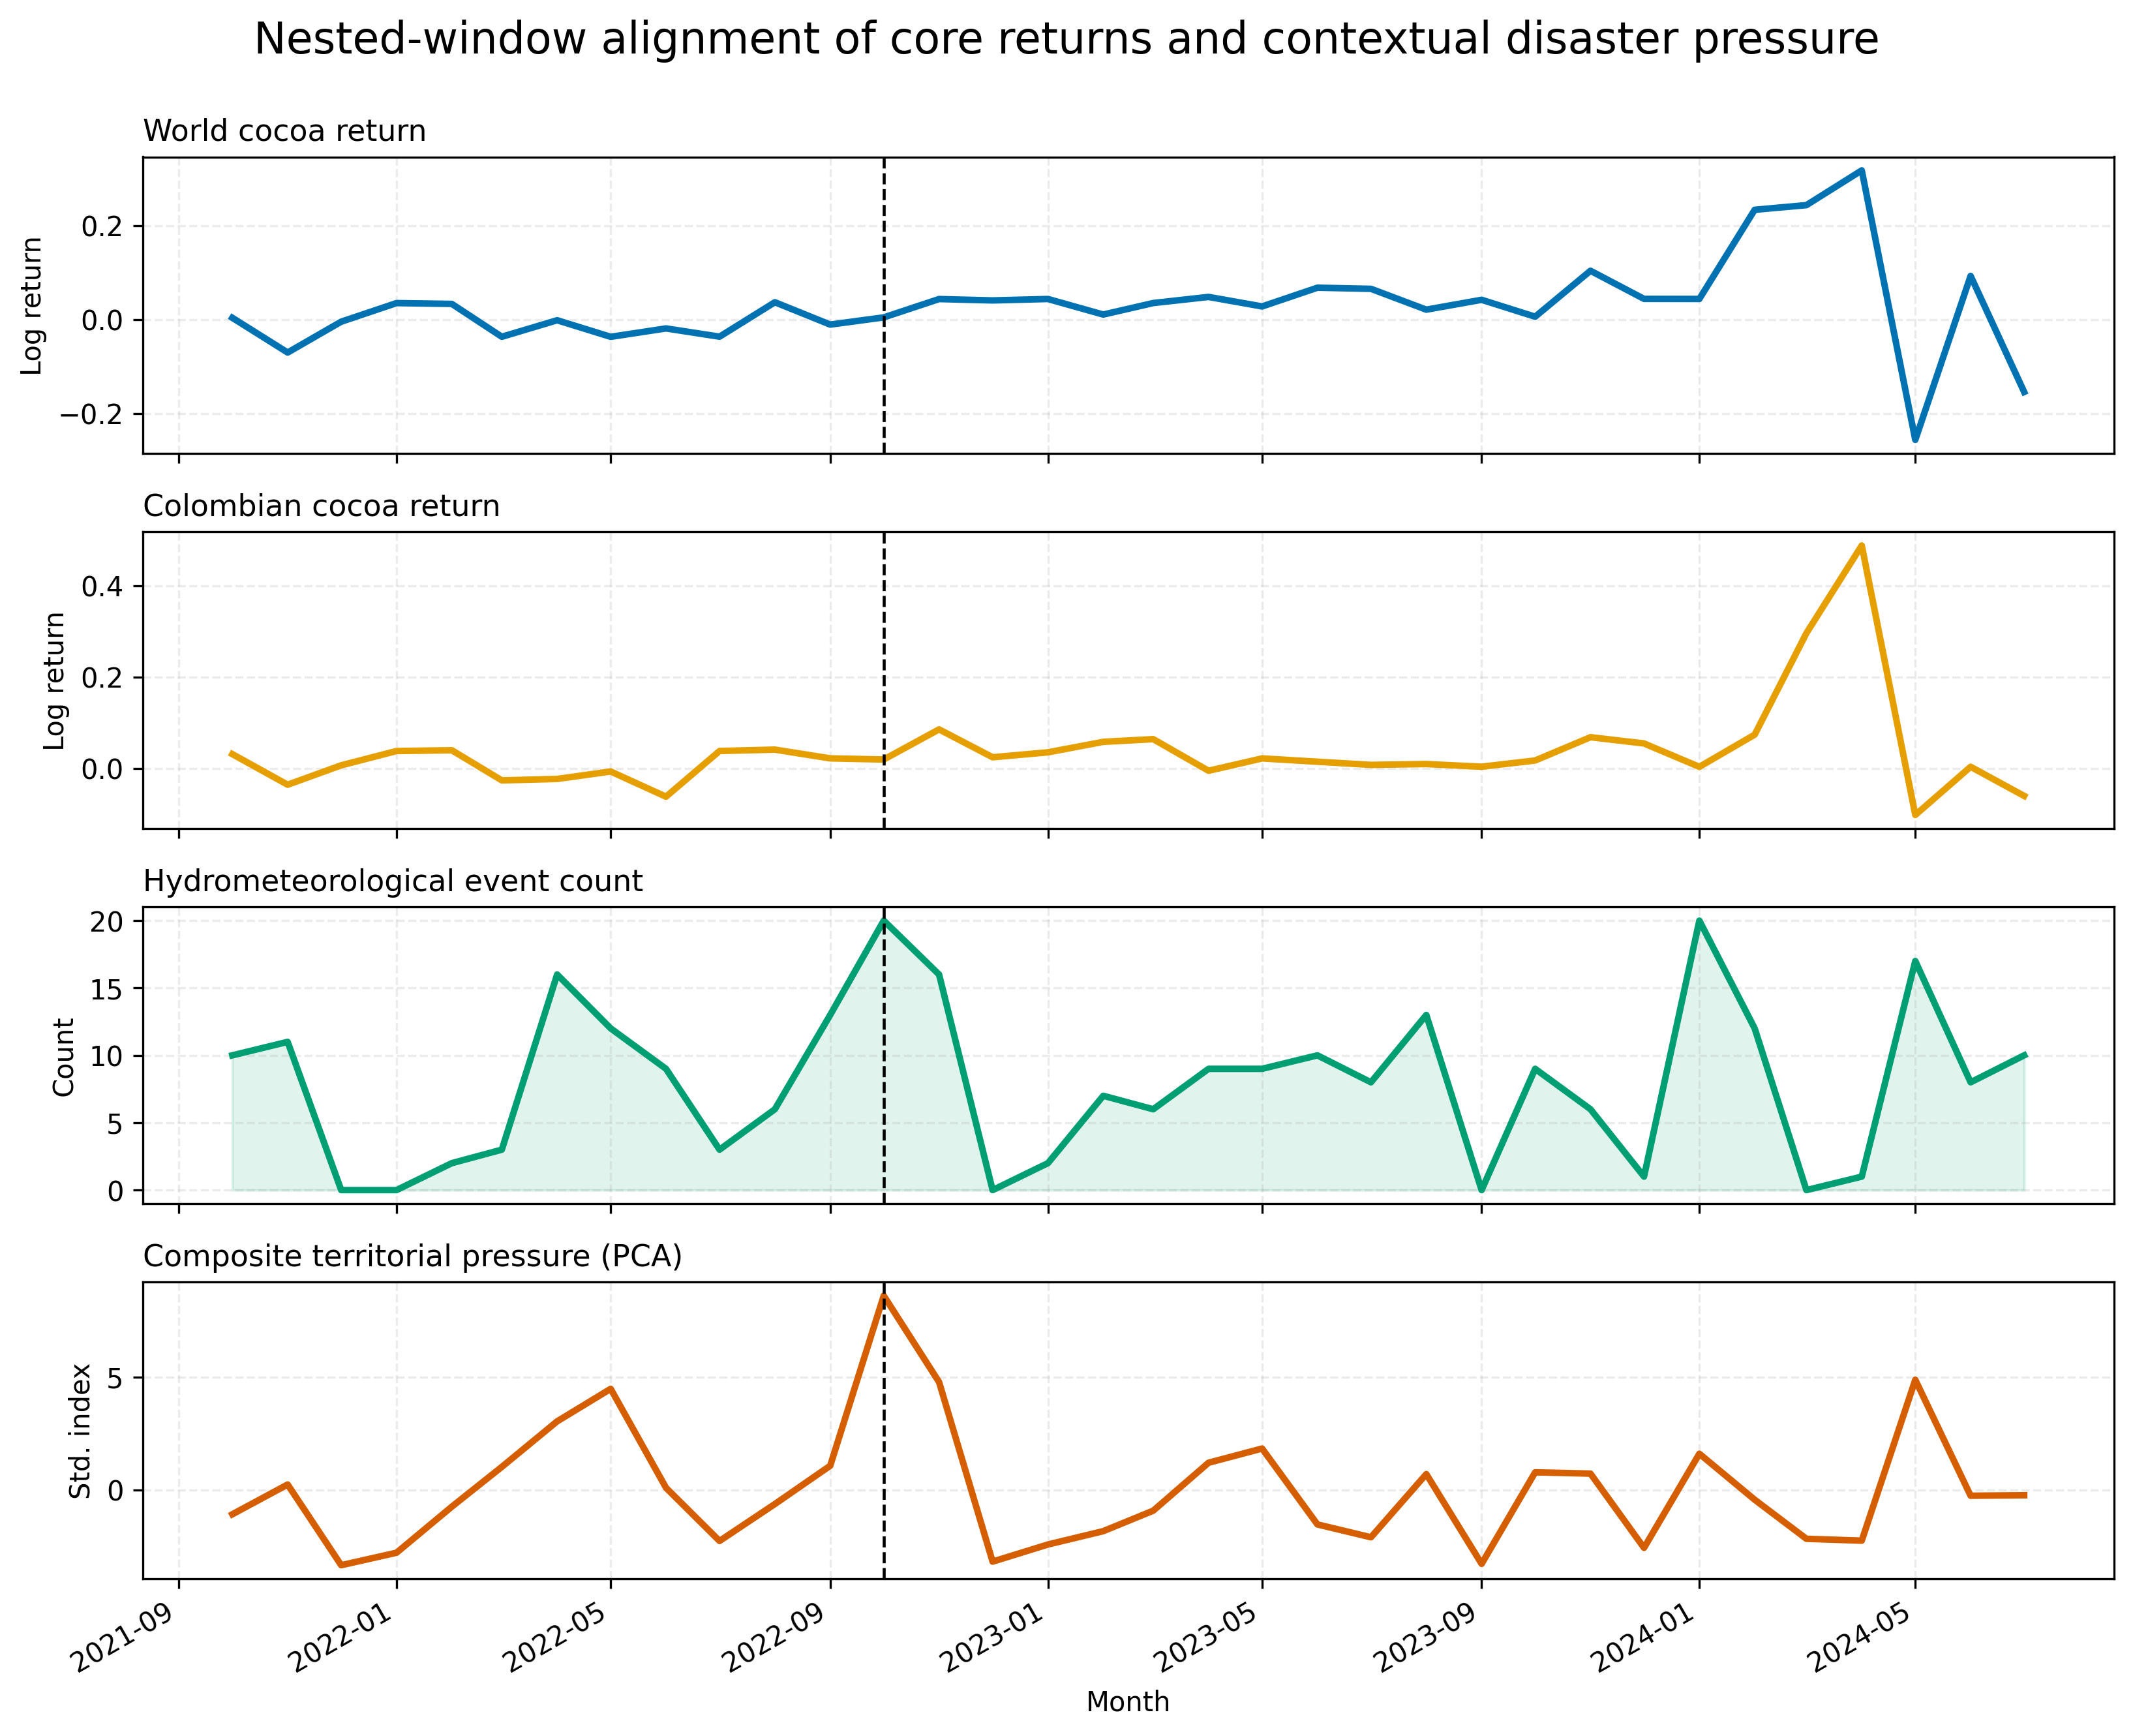
\includegraphics[width=0.94\textwidth]{figures/figure_contextual_overlay_alignment.png}
\caption{Nested return-window alignment of world and Colombian cocoa returns with hydrometeorological counts and the composite territorial-pressure index. The vertical line marks October 2022, the exploratory peak month identified from the hazard screen. The contrast in signal shape underscores that the disaster layer is episodic and contextual rather than benchmark-like.}
\label{fig:contextual_alignment}
\end{figure}

Table~\ref{tab:hazard_screening} formalizes the screening of possible contextual hazard overlays in the 35-month nested return window. Earthquake counts are too sparse to support direct integration: only four months contain earthquake events, and the zero-month share is 0.886. Hydrometeorological events are observed in 30 of the 35 months and peak in October 2022, making them the most viable monthly territorial episode marker among the candidate counts. The PCA pressure index also peaks in October 2022, but it is treated as a synthetic territorial-pressure overlay rather than as a direct count.

\begin{table}[H]
\centering
\caption{Screening of contextual hazard-overlay candidates in the nested return window}
\label{tab:hazard_screening}
\small
\resizebox{\textwidth}{!}{%
\begin{tabular}{p{3.3cm}rrrrrp{2.4cm}p{5.0cm}}
\toprule
Signal & Non-zero months & Zero share & Peak month & Peak value & Corr. with returns & Overlay coefficient & Interpretation decision \\
\midrule
Earthquake counts & 4 & 0.886 & 2022-09 & 1.000 & 0.005 & 0.003 ($p=0.633$) & Screened but too sparse for direct monthly modeling. \\
Hydrometeorological counts & 30 & 0.143 & 2022-10 & 20.000 & -0.366 & -0.015 ($p=0.083$) & Most defensible direct monthly territorial episode marker. \\
Geophysical counts & 28 & 0.200 & 2022-11 & 12.000 & -0.146 & 0.004 ($p=0.613$) & Contextual comparator, not preferred direct episode marker. \\
Total event counts & 35 & 0.000 & 2024-01 & 49.000 & 0.065 & -0.002 ($p=0.823$) & Contextual comparator, not preferred direct episode marker. \\
PCA pressure index & 35 & 0.000 & 2022-10 & 8.613 & -0.277 & -0.004 ($p=0.562$) & Synthetic territorial-pressure overlay, not a causal price driver. \\
\bottomrule
\end{tabular}
}
\end{table}

Table~\ref{tab:hazard_models} then compares the nested-window hazard overlays. These estimates should be read as parsimonious contextual checks rather than as a horse race among co-equal transmission drivers. The hydrometeorological series outperforms the other direct count alternatives in both the return and volatility extensions. Its coefficient is negative and only marginally significant ($p=0.083$ in returns; $p=0.074$ in volatility), so it should not be interpreted as a dominant short-run price setter. Even so, it is more informative than geophysical counts, total monthly events, or the continuous PCA index when the objective is to select one direct territorial episode marker.

\begin{table}[H]
\centering
\caption{Contextual hazard-overlay comparison in the nested return window}
\label{tab:hazard_models}
\small
\resizebox{\textwidth}{!}{%
\begin{tabular}{p{3.5cm}lrrrrrr}
\toprule
Signal & Type & Return adj. $R^2$ & Return coef. & Return $p$ & Vol. adj. $R^2$ & Vol. coef. & Vol. $p$ \\
\midrule
Hydrometeorological events & Direct & 0.653 & -0.015 & 0.083 & 0.935 & -0.003 & 0.074 \\
Geophysical events & Direct & 0.633 & 0.004 & 0.613 & 0.932 & 0.002 & 0.286 \\
Total recorded events & Direct & 0.632 & -0.002 & 0.823 & 0.932 & -0.002 & 0.140 \\
PCA disaster pressure & Composite & 0.633 & -0.004 & 0.562 & 0.932 & -0.002 & 0.264 \\
\bottomrule
\end{tabular}
}
\end{table}

The synthetic robustness overlay nevertheless adds useful information. The first principal component explains 33.1\% of the standardized variance across 21 eligible monthly disaster features, with the largest positive loadings coming from hydrometeorological events, infrastructure impact, affected roads, geophysical events, and housing impact. Its peak occurs in the same month as the hydrometeorological series. Figure~\ref{fig:pca_change_points} shows that the composite indicator and Colombian cocoa returns both intensify around October 2022. The continuous PCA coefficient is weak, but the composite series helps identify a multi-hazard stress episode that is broader than one hazard family alone. The relevant interpretation is contextual: the index summarizes territorial disruption across several dimensions, but it is not treated as a conventional transmission series.

\begin{figure}[H]
\centering
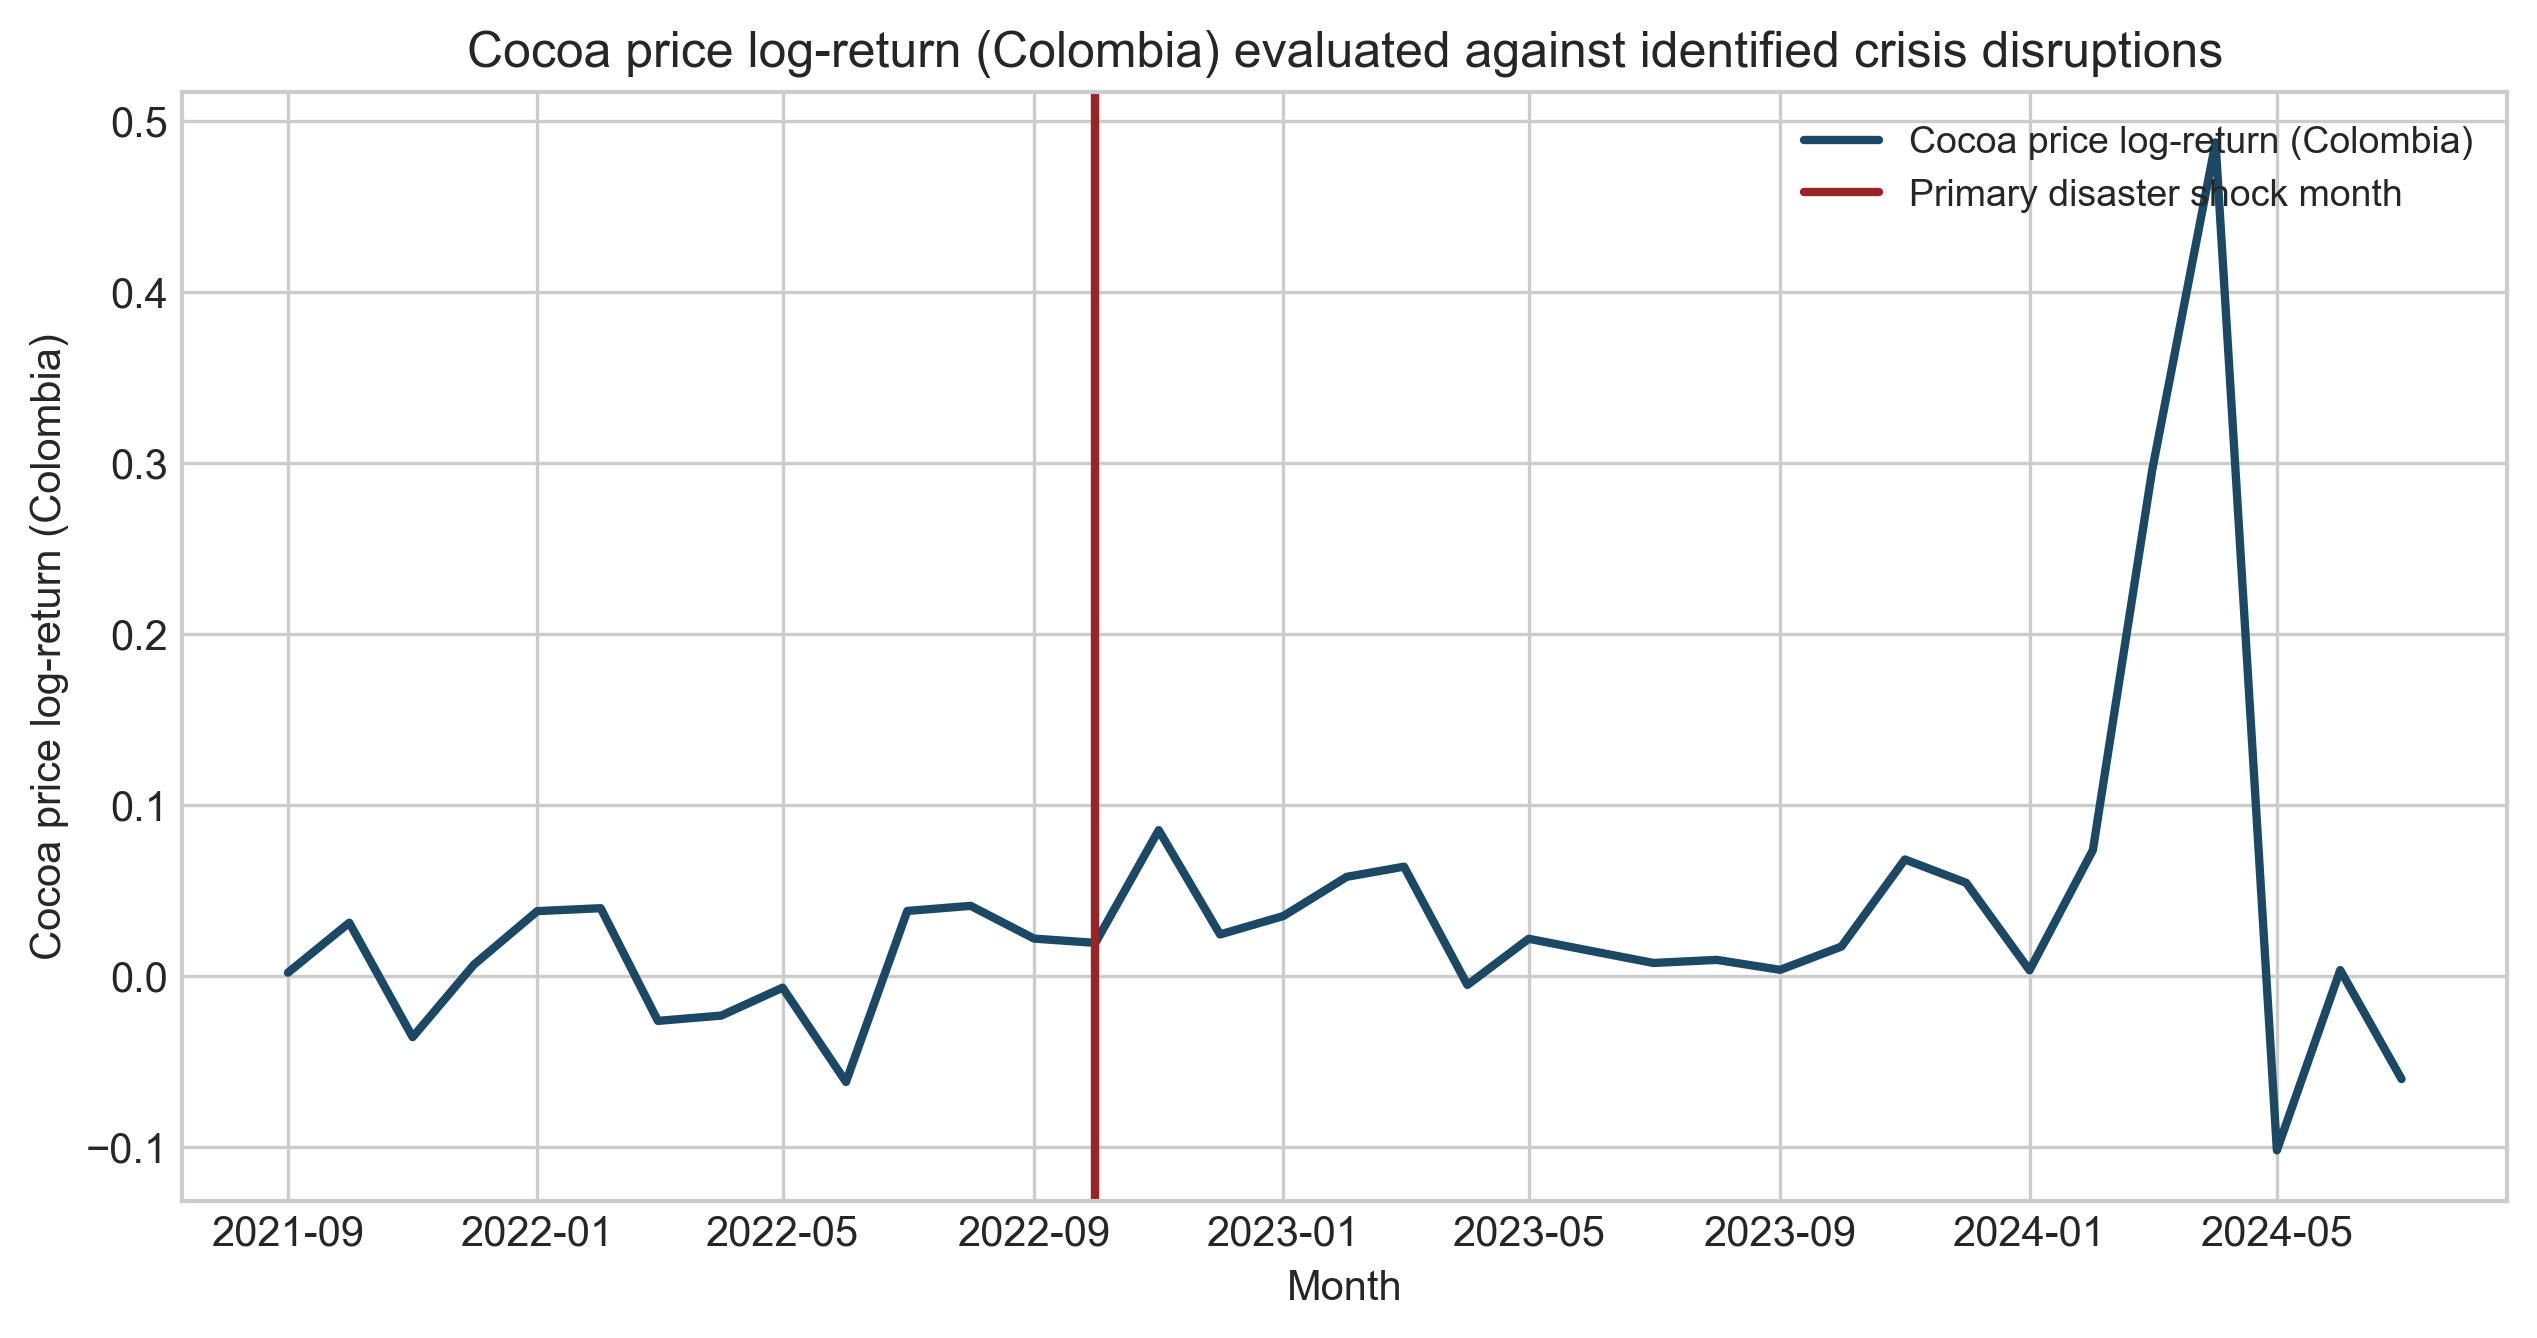
\includegraphics[width=0.85\textwidth]{figures/pca_indicator_change_points.png}
\caption{Composite multi-hazard pressure and cocoa return instability in the nested disaster window. The peak stress episode occurs in October 2022, which also corresponds to the peak month of the direct hydrometeorological event series. The figure is interpreted as an episode-screening tool rather than as evidence of benchmark-like price leadership.}
\label{fig:pca_change_points}
\end{figure}

Table~\ref{tab:mean_shifts} reports the event-window comparison around that peak. Mean domestic returns rise from 0.002 in the six months before October 2022 to 0.044 in the six months after, with a Welch $p$-value of 0.074. Variance and distribution shifts are weaker. The implication is not that the event window proves a disaster effect, but that the disaster overlay is more visible as a discrete stress episode than as a stable linear marginal effect. Because October 2022 was selected from the same nested hazard data used in the screen, this comparison should be read as exploratory episode stratification rather than as exogenous shock identification. It is therefore used only to motivate a cautious resilience-dividend discussion.

\begin{table}[H]
\centering
\caption{Exploratory event-window comparison around the October 2022 peak contextual-pressure month}
\label{tab:mean_shifts}
\small
\begin{tabular}{lrrrrrr}
\toprule
Event month & Window & Pre mean & Post mean & Welch $p$ & Levene $p$ & KS $p$ \\
\midrule
2022-10 & 6 months & 0.002 & 0.044 & 0.074 & 0.546 & 0.474 \\
\bottomrule
\end{tabular}
\end{table}

\section{Discussion}
\label{sec:discussion}

The integrated article shows that resilience in the cocoa chain cannot be reduced to a climatic narrative or to a market narrative alone. The strongest and most stable result remains benchmark transmission: Colombian producer-linked prices move closely with world cocoa prices, and that short-run link is economically large. In vulnerability terms, this means that Santander smallholders operate as price takers in a global system whose benchmark shocks are transmitted quickly to the producer-linked layer. That observation grounds the resilience argument in an observable mechanism of exposure rather than in a purely rhetorical claim \citep{Turner2003,Adger2006,TsowouGayi2019}.

The downstream results reinforce the same point from another angle. The European chocolate index shows a positive levels association with the benchmark but far weaker return adjustment. This does not prove a full downstream insulation mechanism, and the aligned sample is too short to support strong chain-wide structural claims. Even so, the contrast is consistent with an uneven-adjustment interpretation in which producer-linked prices absorb benchmark volatility more directly than the downstream consumer layer. In resilience terms, the question is not simply whether volatility exists, but where it is absorbed and whose livelihoods are exposed when shocks arrive.

Environmental stress does not overturn that transmission logic, but it changes how the transmission results should be interpreted. The weather block improves model fit only slightly, which argues against recasting the article as a weather-dominant price model. At the same time, the full-window stress indicators show that benchmark-driven exposure often occurs under locally unfavorable natural-capital conditions. The nested disaster extension sharpens the point further. Among the direct hazard candidates, hydrometeorological counts are the most defensible monthly territorial episode marker, and they peak in the same month as the multi-hazard PCA indicator. Their negative coefficients in the nested overlay models are suggestive rather than definitive, but they are consistent with the possibility that local disruption weakens the local realization of otherwise benchmark-driven price movements through marketing, logistics, or timing constraints. The October 2022 window reinforces the interpretation that territorial shocks matter more as crisis windows than as stable month-to-month price setters, but the reproducible comparison remains suggestive rather than confirmatory.

This is where the ecological-economics framing becomes useful. The paper's contribution is not to claim that disasters directly determine cocoa prices in a short monthly sample. It is to show that vulnerability emerges from the coupling of market transmission and territorial stress. Benchmark transmission defines the exposure channel; local weather anomalies, hydrometeorological disruption, and multi-hazard event pressure condition the sensitivity and buffering capacity of the local system. The article therefore extends a standard market-integration study into a socio-ecological interpretation without overstating causal inference.

Several methodological cautions are central to that interpretation. The PCA disaster indicator is not directly comparable to world cocoa, exchange-rate, or oil prices. It is a synthetic territorial-pressure construct built from heterogeneous event, damage, and spread variables, of the kind often used in disaster-risk assessment to summarize contextual exposure rather than market dynamics \citep{Parsons2021,Garschagen2021}. Likewise, the monthly hydrometeorological count is an irregular registry-based count process, not a canonical continuous price series. Weak coefficients, weak Granger evidence, or isolated pairwise correlations therefore do not justify presenting the disaster layer as a dominant driver of the market system. The shorter disaster window is substantively important here: with only 35 return observations, sparse event counts, and heterogeneous indicator construction, a large multivariate transmission model would imply more comparability than the data can support \citep{hakkio_rush_1991,lutkepohl_2005}.

The event-window evidence should be read with the same discipline. October 2022 was selected from the same nested hazard data used to identify the most viable direct overlay, so the resulting comparison is exploratory rather than strictly exogenous. There is also a scale mismatch between the departmental disaster registry, the point-based weather series, and the broader producer-linked price system. Those limits do not eliminate the relevance of territorial disruption, but they do narrow the claim: the disaster layer helps identify periods in which benchmark pass-through is experienced under adverse local conditions; it does not establish a disaster-led short-run price process.

The event-window evidence is therefore not interpreted as proof that agroforestry caused lower volatility, nor as an empirical contrast between agroforestry and monoculture areas. No farm-level land-use, shade-density, or monoculture-comparison dataset was found in the repository inputs. Rather, the event window identifies a period in which benchmark exposure and territorial pressure coincided. Within the resilience framework, agroforestry and diversified livelihood systems represent potential buffer capacities that may generate a resilience dividend by reducing the likelihood that market and environmental shocks translate into livelihood collapse \citep{Mechler2025}. Empirical validation of that mechanism would require farm-level or land-use data that are not available in the present design.

That narrower claim is still substantively meaningful. Resilience scholarship emphasizes that local coping capacity, infrastructure, and governance condition how shocks are absorbed even when those shocks originate elsewhere \citep{Djalante2011,Birkmann2023}. The present results fit that pattern. A price shock and a territorial disruption do not need to be identical in form to interact. Benchmark transmission can remain the main exposure mechanism while territorial disruption amplifies how that exposure is experienced by smallholders, cooperatives, and local traders.

The weak short-run exchange-rate coefficient in the return model also deserves a cautious institutional interpretation. One plausible explanation is that sector coordination, contracting practices, or price-setting arrangements dampen immediate currency pass-through even when world cocoa benchmarks remain dominant. This interpretation is not directly observed in the present data and should therefore remain conditional. Even so, it points toward a practical resilience question: institutional arrangements may not eliminate exposure to world benchmarks, but they may influence how quickly secondary shocks are transmitted to producers.

\subsection{Basis Risk, Territorial Blindness, and Financial Equity}

The integrated results also clarify a policy-relevant form of basis risk. In this setting, basis risk is the mismatch between global benchmark prices or national-level financial indicators and localized disruptions such as landslides, road failures, buyer-access interruptions, harvest-circulation constraints, and municipal disaster pressure. A benchmark-linked price-risk tool may track the world cocoa signal well while still missing the local conditions that determine whether a smallholder can harvest, transport, store, sell, or obtain temporary liquidity during a stress episode. The evidence markers supporting this interpretation are not causal policy estimates; they are the coexistence of strong benchmark transmission, hydrometeorological event concentration, PCA pressure peaks, natural-capital anomaly months, and clear scale mismatch between the departmental disaster registry, point-based weather data, and producer-linked price series.

This territorial blindness matters for financial equity. Instruments designed only around benchmark prices may be poorly aligned with the stress experienced by producers whose losses arise through road access, delayed buyer visits, damaged local infrastructure, or emergency cash constraints rather than through the benchmark itself. The policy implication is that benchmark-linked price-risk tools should be complemented by decentralized resilience funds or territorial-risk financing instruments tied to local stress indicators. Such instruments could support emergency logistics, rural road maintenance after hydrometeorological events, temporary liquidity for producer households or cooperatives, cooperative storage, and coordinated transport when buyer access is interrupted. The paper does not prove that these instruments work; it shows why territorial stress indicators should be considered alongside benchmark exposure when designing them.

Several limitations remain. The core aligned return sample contains 52 monthly observations, and the nested disaster return window contains only 35. That is enough for transparent reduced-form analysis, hazard screening, and event-window comparisons, but not for strong claims from large multivariate cointegration systems. The Colombian domestic price series is a national reference price rather than a farm-gate panel, and the weather block is location-based rather than household-specific. The disaster registry is rich enough for monthly aggregation, but still short for finely identified dynamic hazard models. These limits argue for empirical modesty, not for abandoning the resilience question.

Even with those constraints, the integrated findings yield practical lessons. Resilience-enhancing arrangements in cocoa-producing territories are unlikely to come from adaptation planning alone if benchmark transmission remains the dominant exposure mechanism. Risk-sharing instruments, cooperative coordination, storage and marketing support, contract duration, diversification, and local early-warning systems are more plausibly complementary than competing responses. For territorial governance, the main implication is that market shocks and environmental disruption should be monitored together rather than treated as separate policy files.

\section{Conclusion}
\label{sec:conclusion}

This article integrates two earlier manuscript versions into one publication-oriented analysis of cocoa price transmission and territorial resilience in Santander, Colombia. The main conclusion is clear: international cocoa benchmarks remain the dominant short-run driver of Colombian producer-linked prices, but the vulnerability implications of that transmission are better understood when environmental stress is incorporated into the design. Weather anomalies matter mainly as natural-capital stress proxies. The structural-break diagnostic retains the no-break benchmark by BIC, which cautions against claiming an observed tipping point in the short aligned sample. In the shorter disaster window, hydrometeorological event counts provide the most defensible monthly territorial episode marker, while the PCA-based multi-hazard index remains useful as a robustness overlay and event-screening device. The October 2022 peak shared by both signals is associated with a higher post-window mean return, but the evidence is exploratory and the disaster layer is better interpreted as contextual territorial exposure than as a co-equal transmission series.

The contribution is therefore a layered resilience methodology with methodological restraint, not a disaster-led pricing model. The paper shows how a benchmark-transmission framework can be linked to resilience analysis without making claims beyond what the data support. The approach is most transferable to territories and commodities where producers are tightly tied to global benchmarks and also exposed to recurrent environmental disruption under short and uneven overlap. Stronger claims require longer disaster windows, local price histories, farm-gate panels, independently identified hazard episodes, and farm-level buffer-capacity data, especially on land use, agroforestry density, cooperative access, and liquidity constraints. For now, the most defensible practical lesson is that producer resilience requires attention to both price transmission and territorial exposure, including coordination mechanisms, diversification, early-warning systems, territorial-risk financing, and adaptation planning that treats these dimensions as connected.

\clearpage
\section*{Supplementary Display Items}

The following supplementary figures and tables preserve the diagnostic evidence base developed across the first two manuscript versions. Items that became redundant in the main text were retained here rather than discarded.

\begin{figure}[H]
\centering
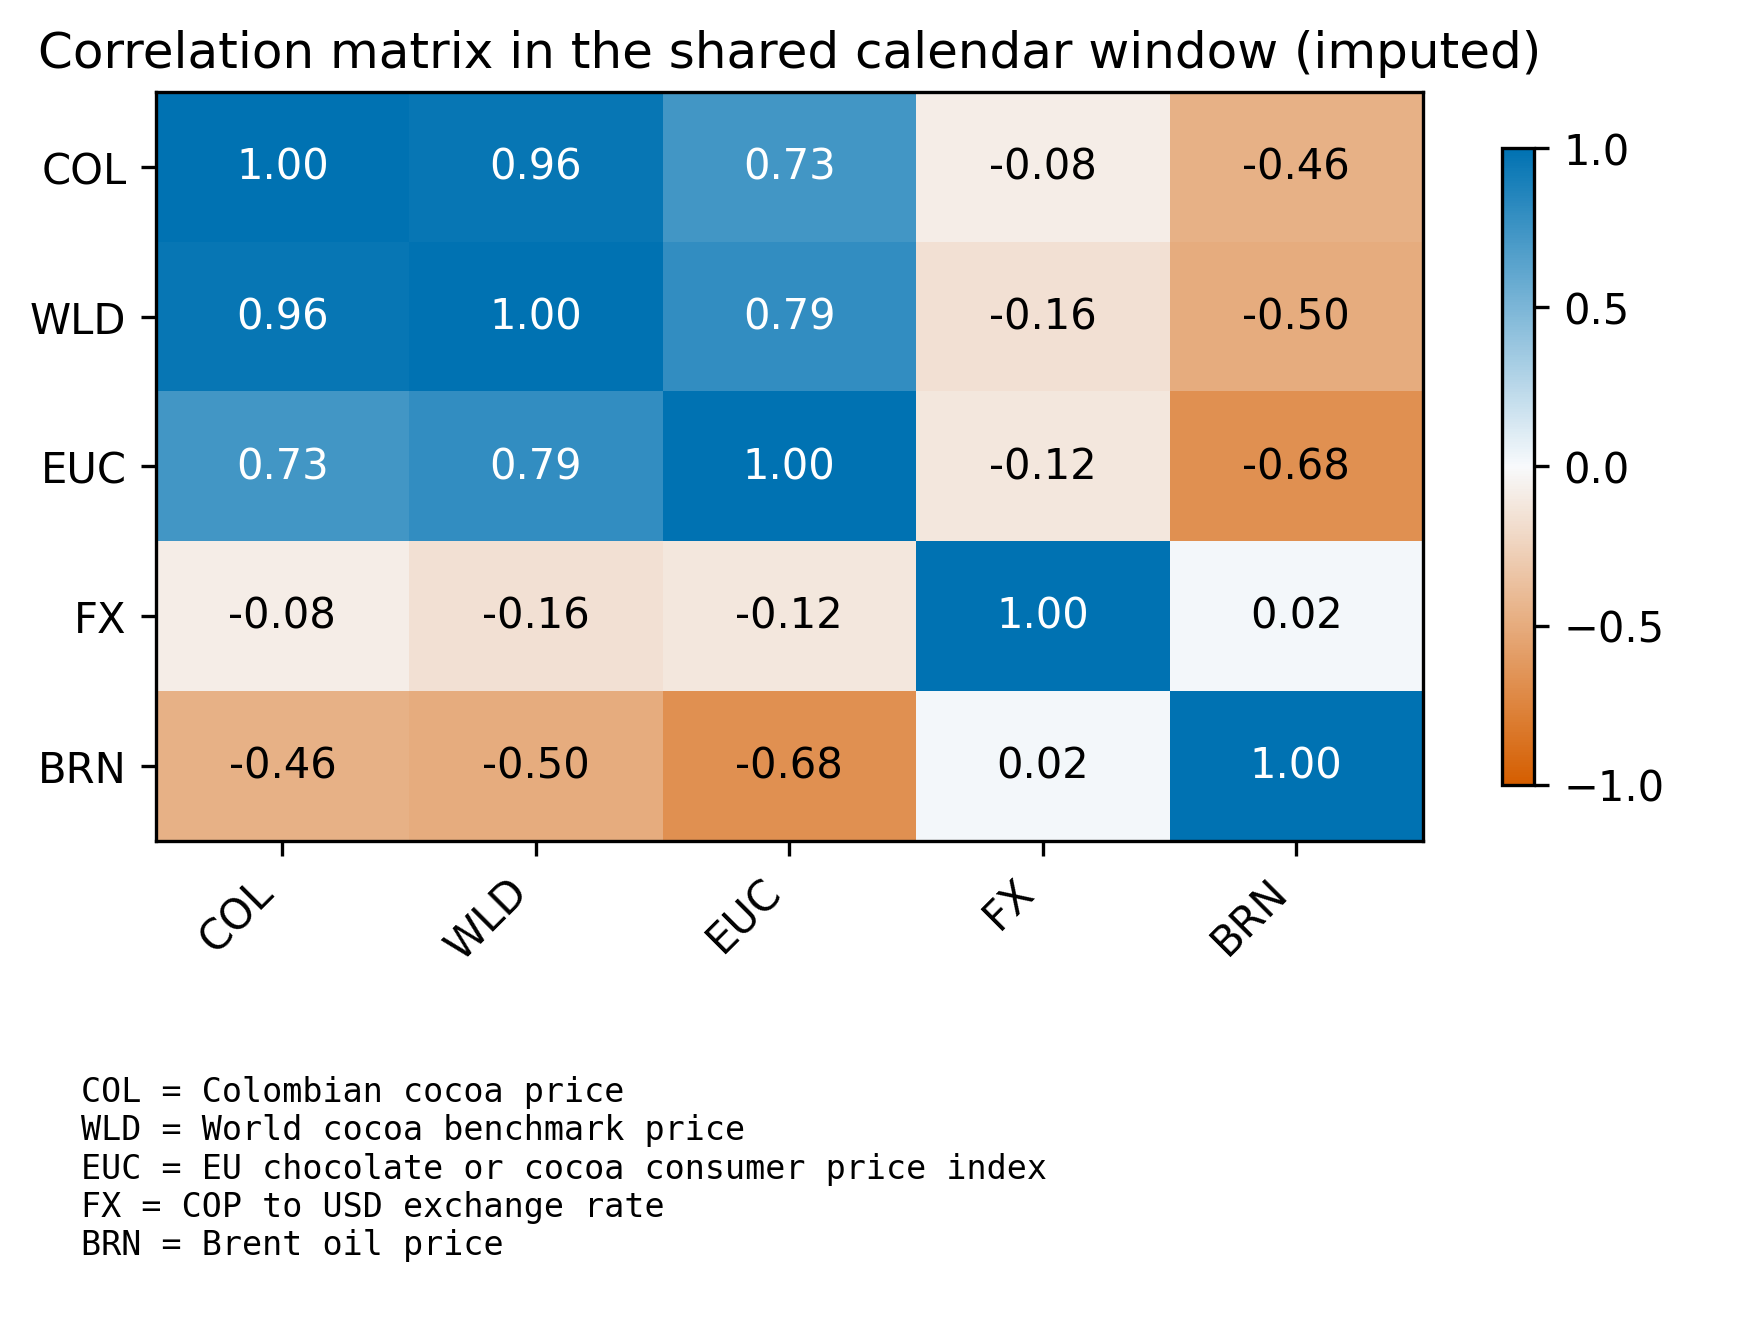
\includegraphics[width=0.90\textwidth]{figures/figure_correlation_heatmap_levels_common_window_imputed.png}
\caption{Core-system level correlation heatmap retained from the first manuscript version. The display preserves the original descriptive evidence on the dependence structure of the benchmark, domestic, downstream, exchange-rate, and oil series.}
\label{fig:supp_core_corr}
\end{figure}

\begin{figure}[H]
\centering
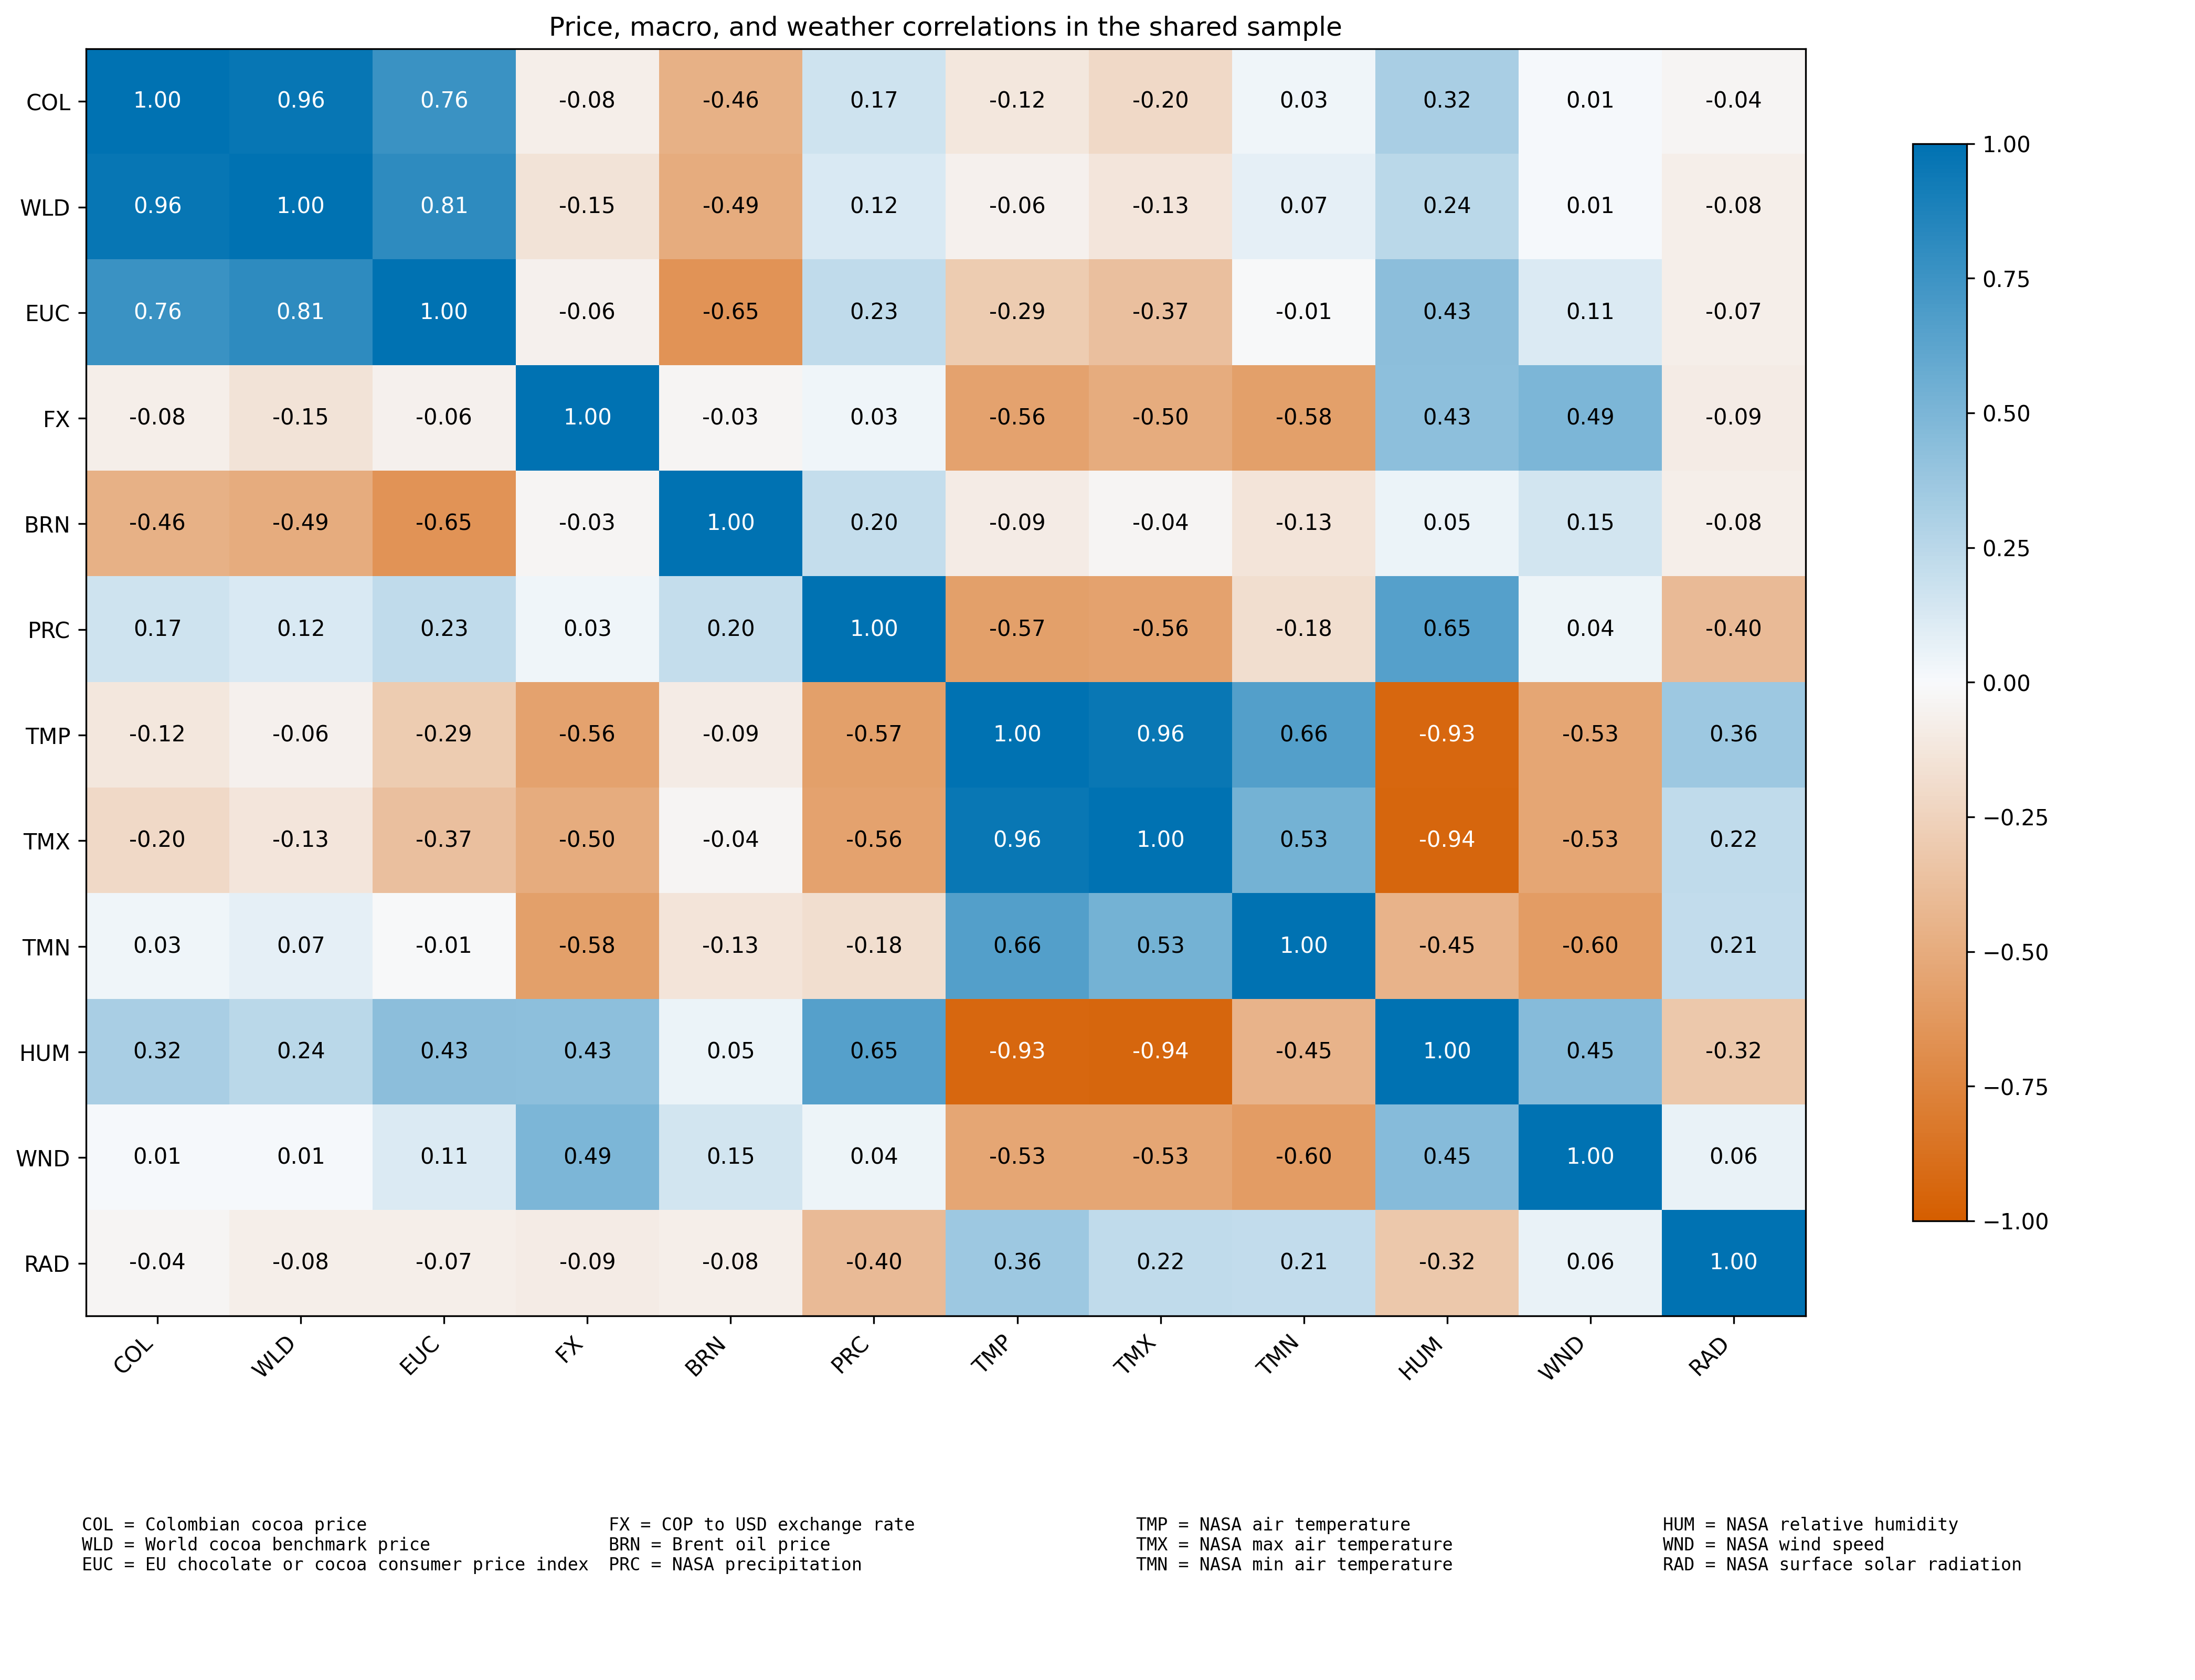
\includegraphics[width=\textwidth]{figures/figure_climate_core_correlation_common_sample.png}
\caption{Climate-core correlation matrix retained from the first manuscript version. The figure preserves the original bridge between the price system and the local weather block without requiring a large unstable climate-augmented VAR.}
\label{fig:supp_climate_corr}
\end{figure}

\begin{figure}[H]
\centering
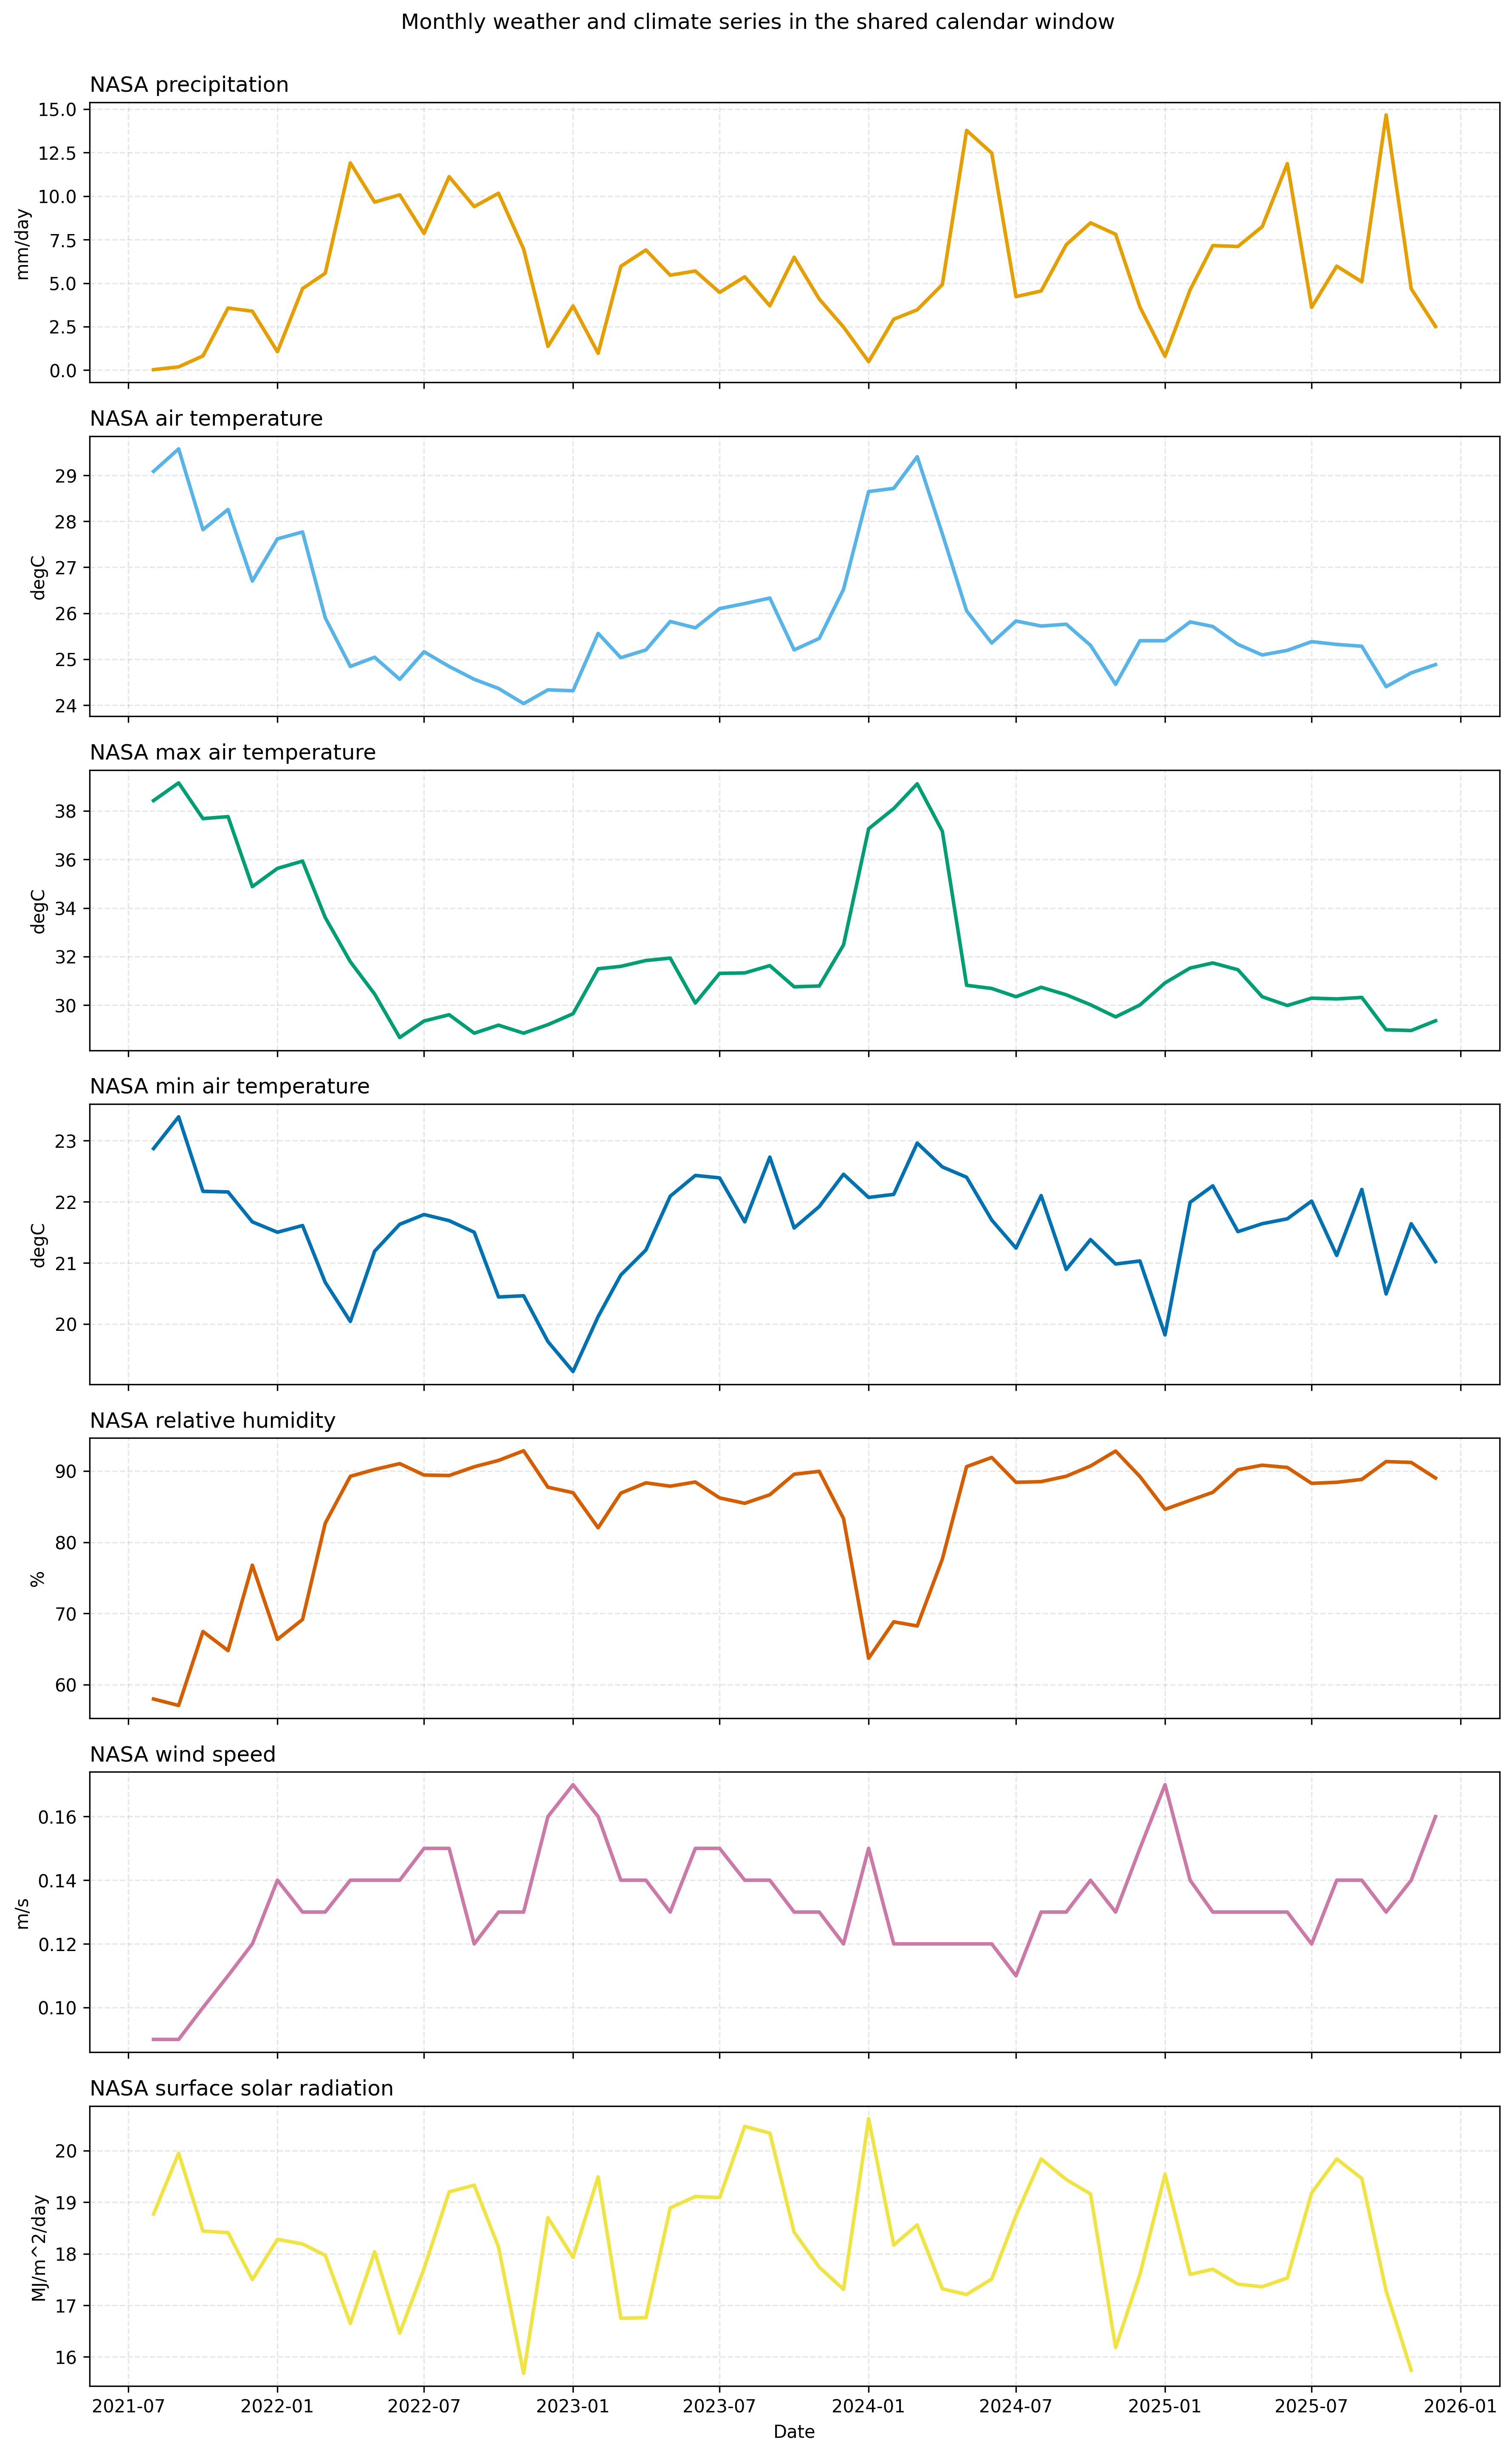
\includegraphics[width=\textwidth,height=0.82\textheight,keepaspectratio]{figures/figure_climate_series_panels_common_window.png}
\caption{Climate series panels for San Vicente de Chucuri retained from the first manuscript version. These panels preserve the underlying environmental context summarized more compactly by the main-text weather-stress figure.}
\label{fig:supp_climate_panels}
\end{figure}

\begin{figure}[H]
\centering
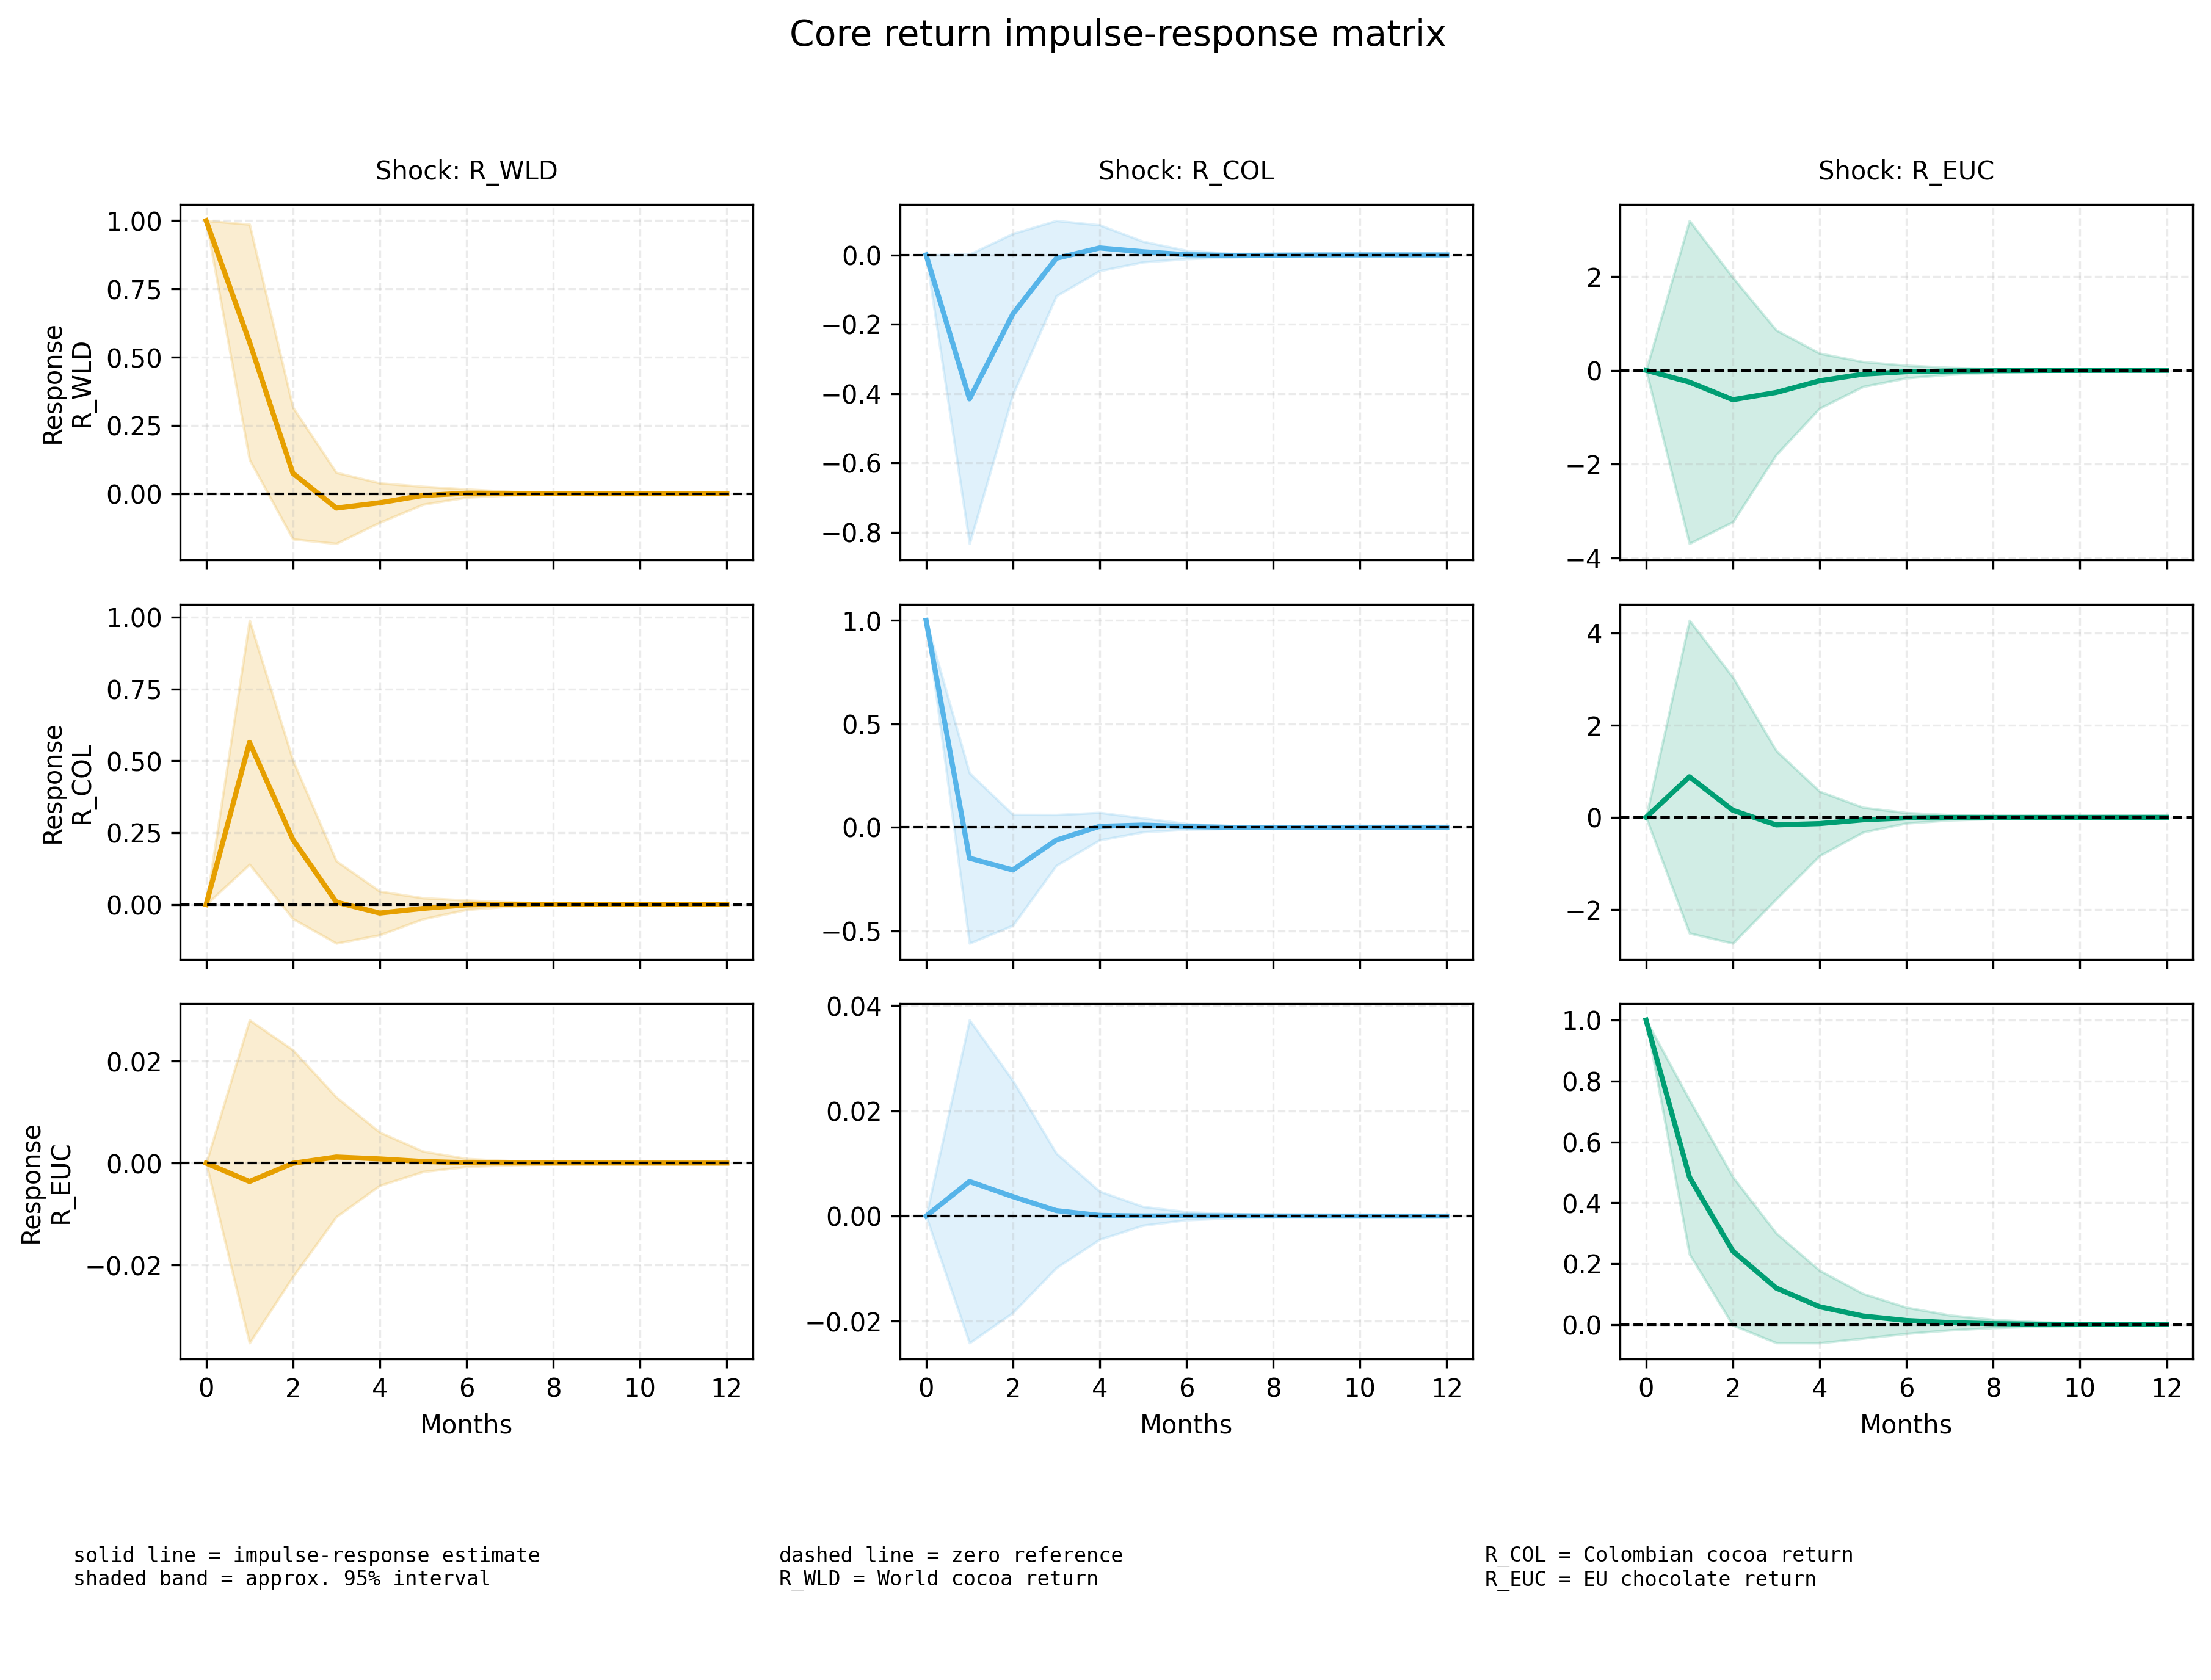
\includegraphics[width=\textwidth]{figures/figure_core_return_impulse_response.png}
\caption{Compact return-VAR impulse-response matrix retained from the first manuscript version. Because the aligned sample is short, the article treats this figure as supplementary reduced-form evidence rather than as a headline causal result.}
\label{fig:supp_irf}
\end{figure}

\begin{figure}[H]
\centering
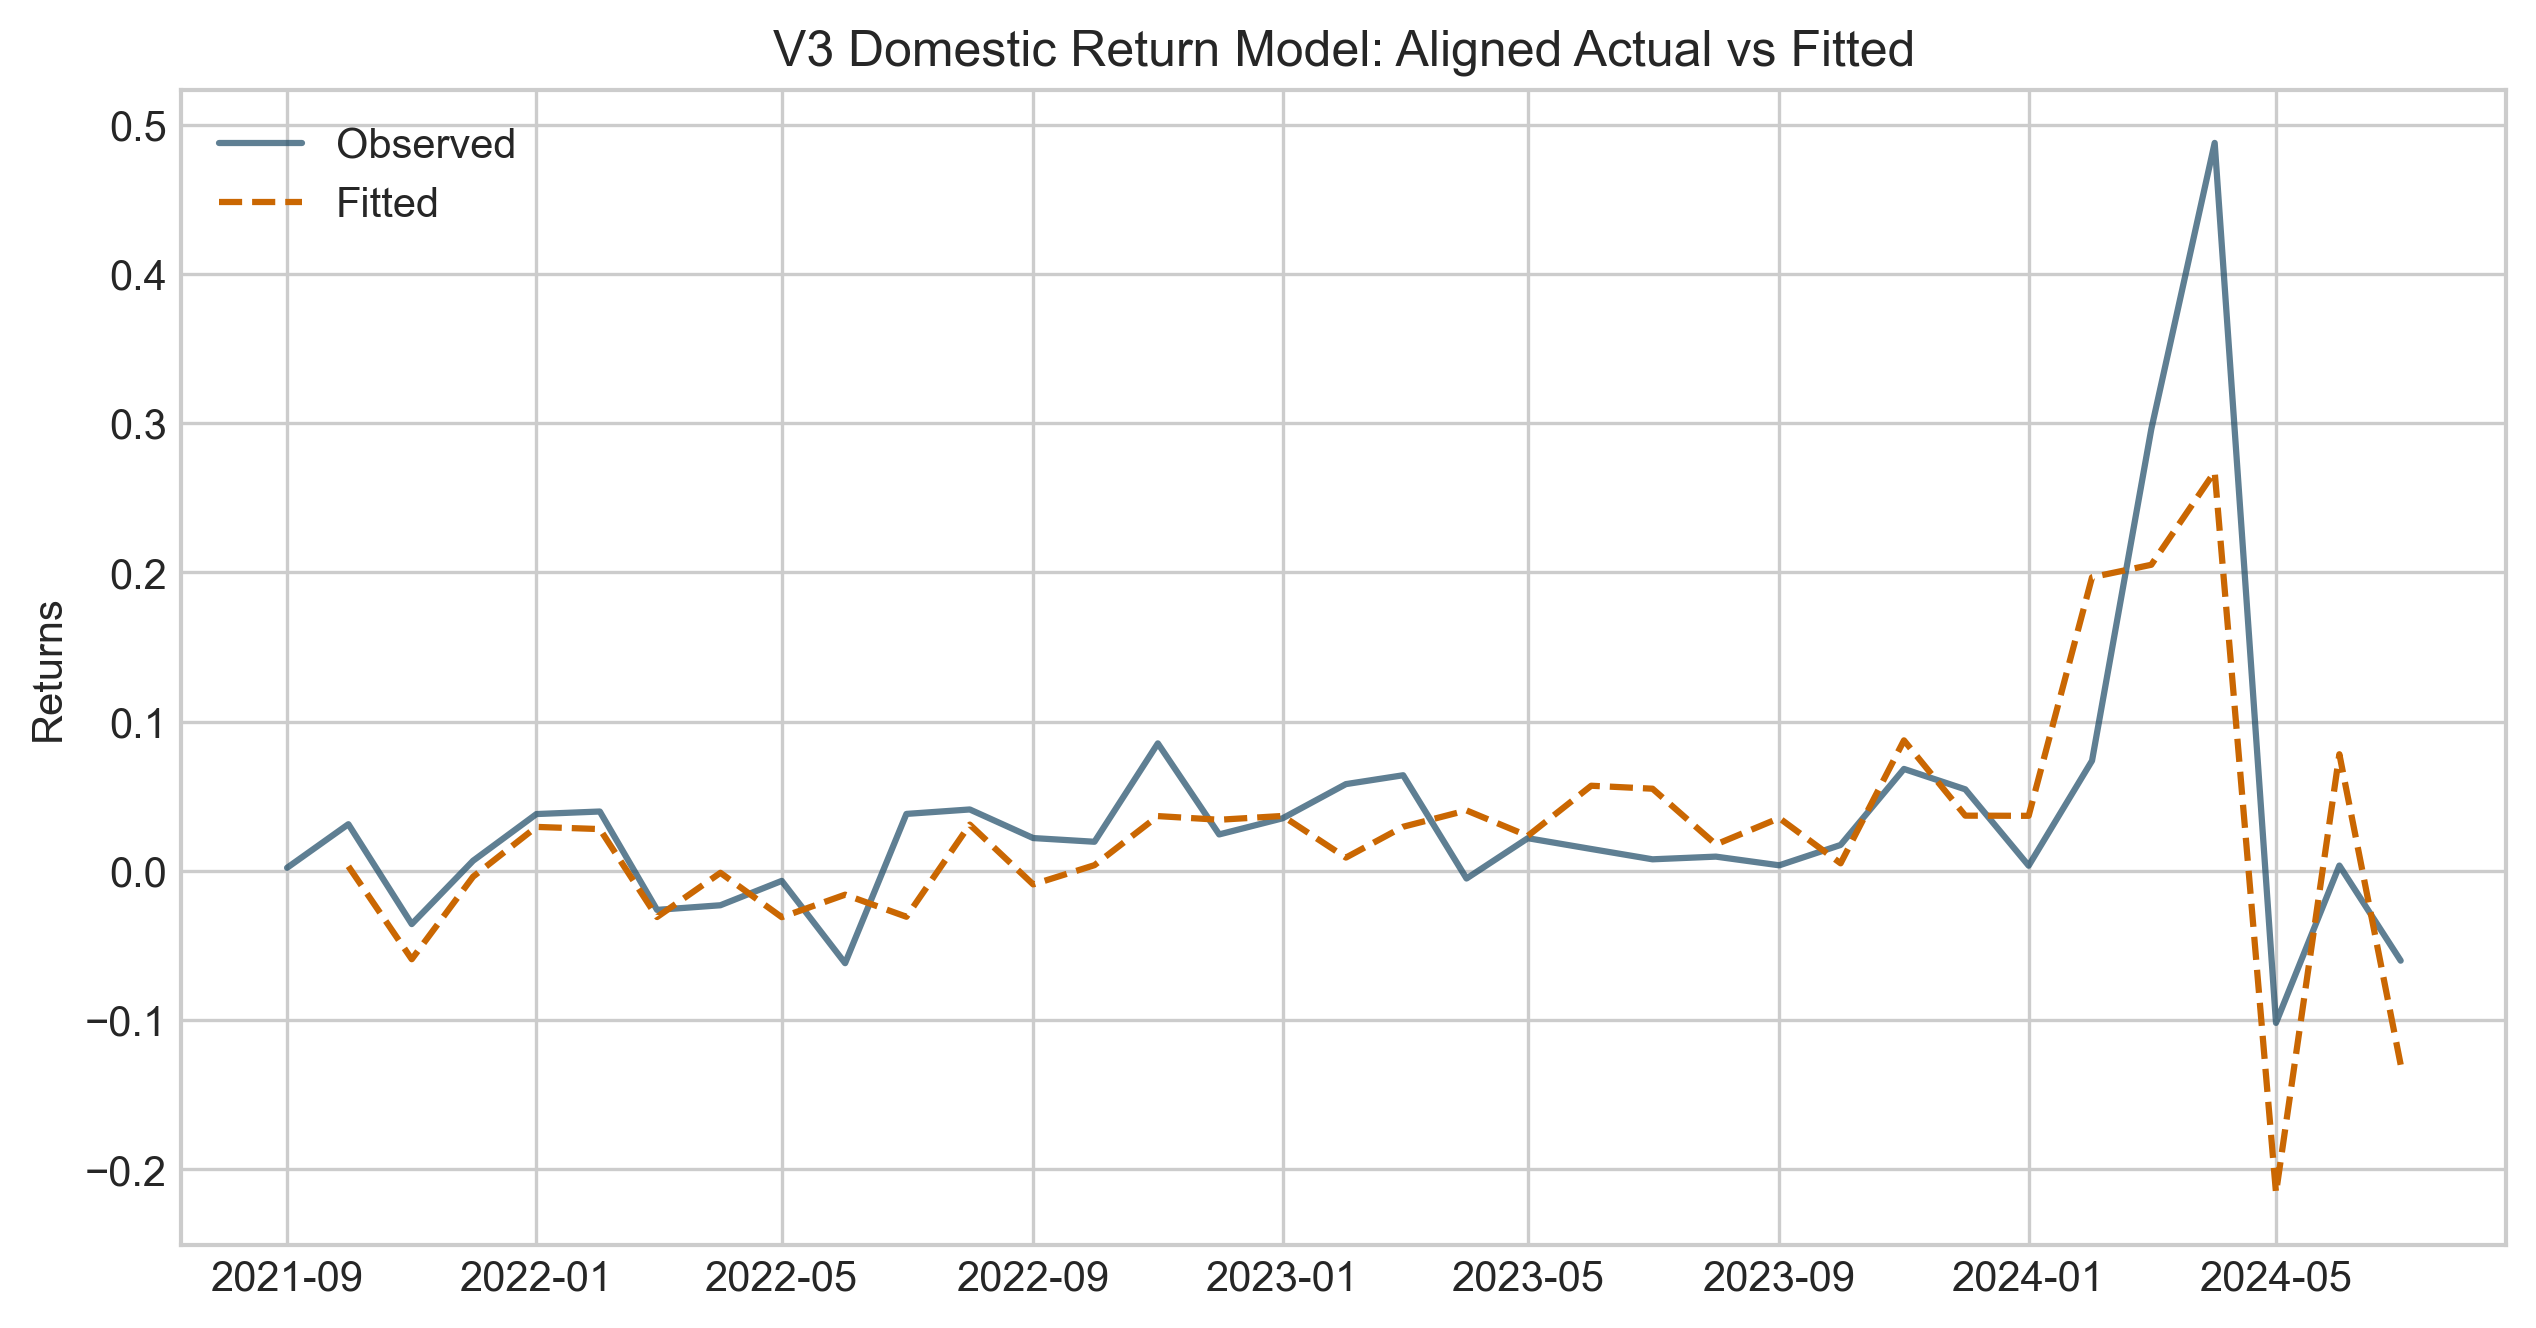
\includegraphics[width=0.90\textwidth]{figures/figure_v3_actual_vs_fitted.png}
\caption{Actual-versus-fitted domestic return model from the disaster-extension manuscript. The figure is retained as a supplementary model-diagnostic display after the main article shifted the emphasis toward hazard screening and event-window interpretation.}
\label{fig:supp_actual_fitted}
\end{figure}

\begin{figure}[H]
\centering
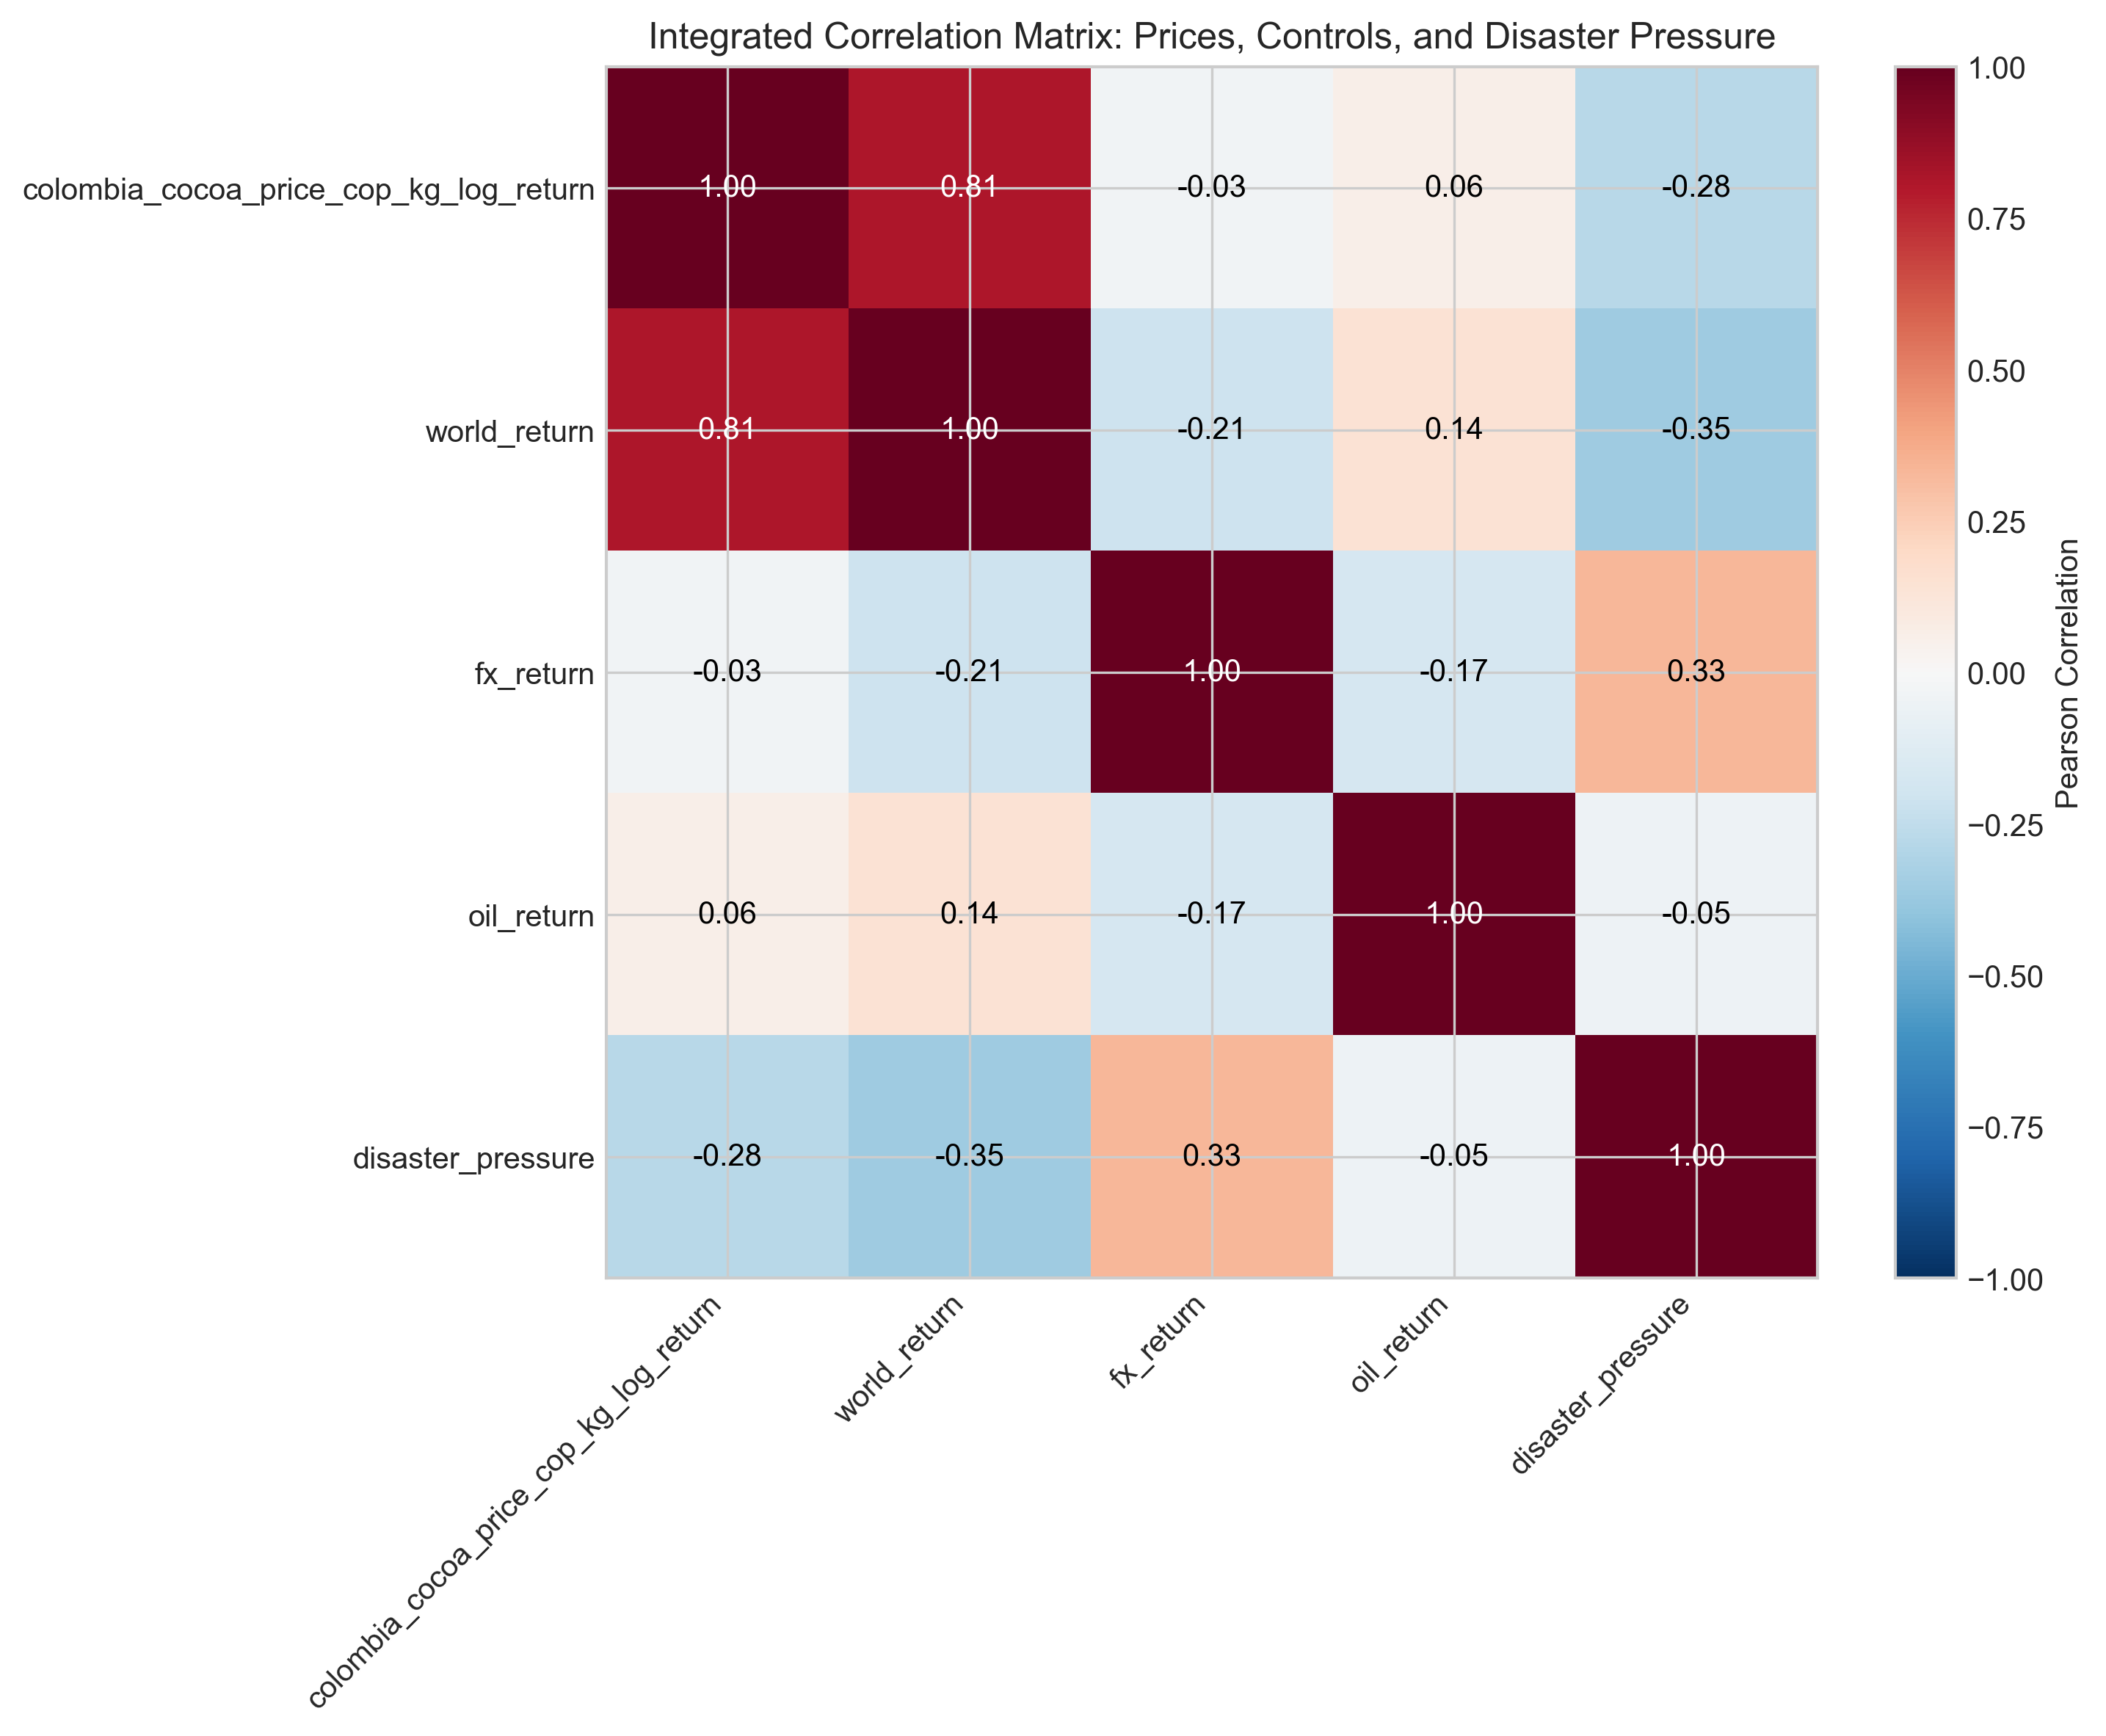
\includegraphics[width=0.82\textwidth]{figures/figure_v3_integrated_heatmap.png}
\caption{Integrated correlation matrix from the disaster-extension manuscript. The figure is retained to preserve the original pairwise descriptive view of returns, macro controls, and composite disaster pressure.}
\label{fig:supp_integrated_heatmap}
\end{figure}

\begin{figure}[H]
\centering
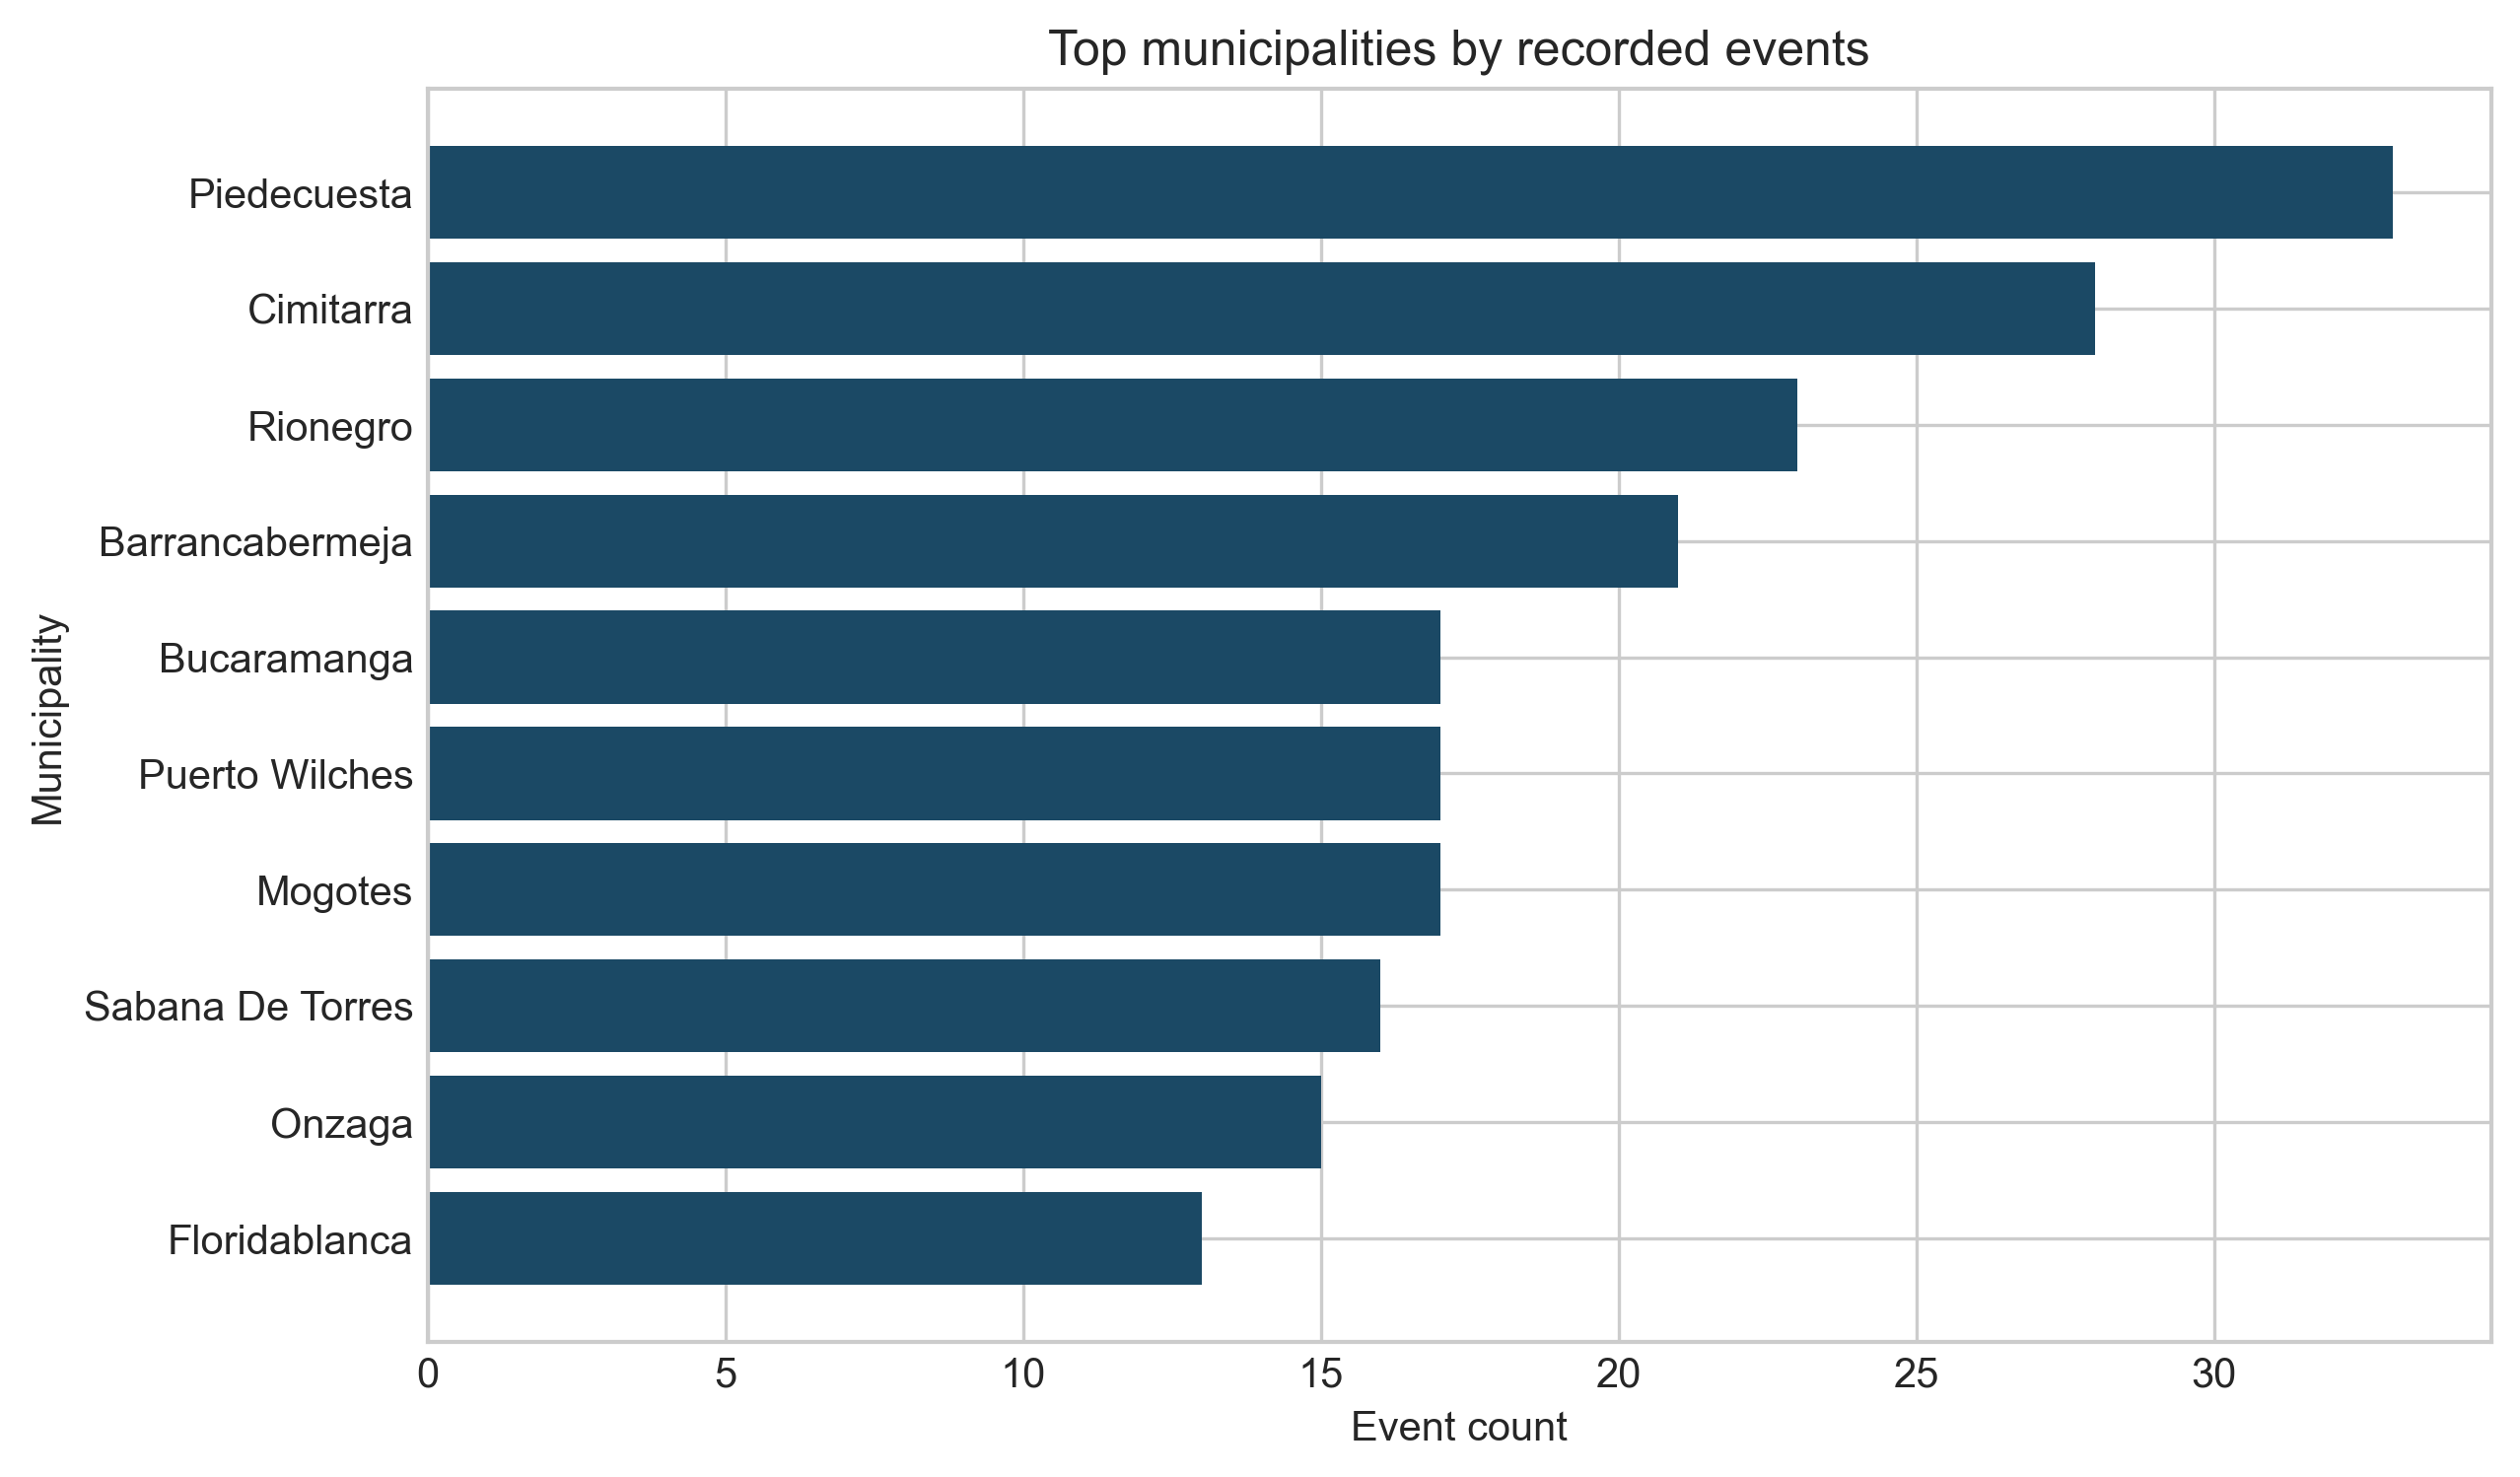
\includegraphics[width=0.80\textwidth]{figures/figure_top_municipalities.png}
\caption{Top municipalities by recorded events retained from the disaster-extension manuscript. The figure is kept as supplementary territorial detail rather than as a main-text result.}
\label{fig:supp_municipalities}
\end{figure}

\begin{figure}[H]
\centering
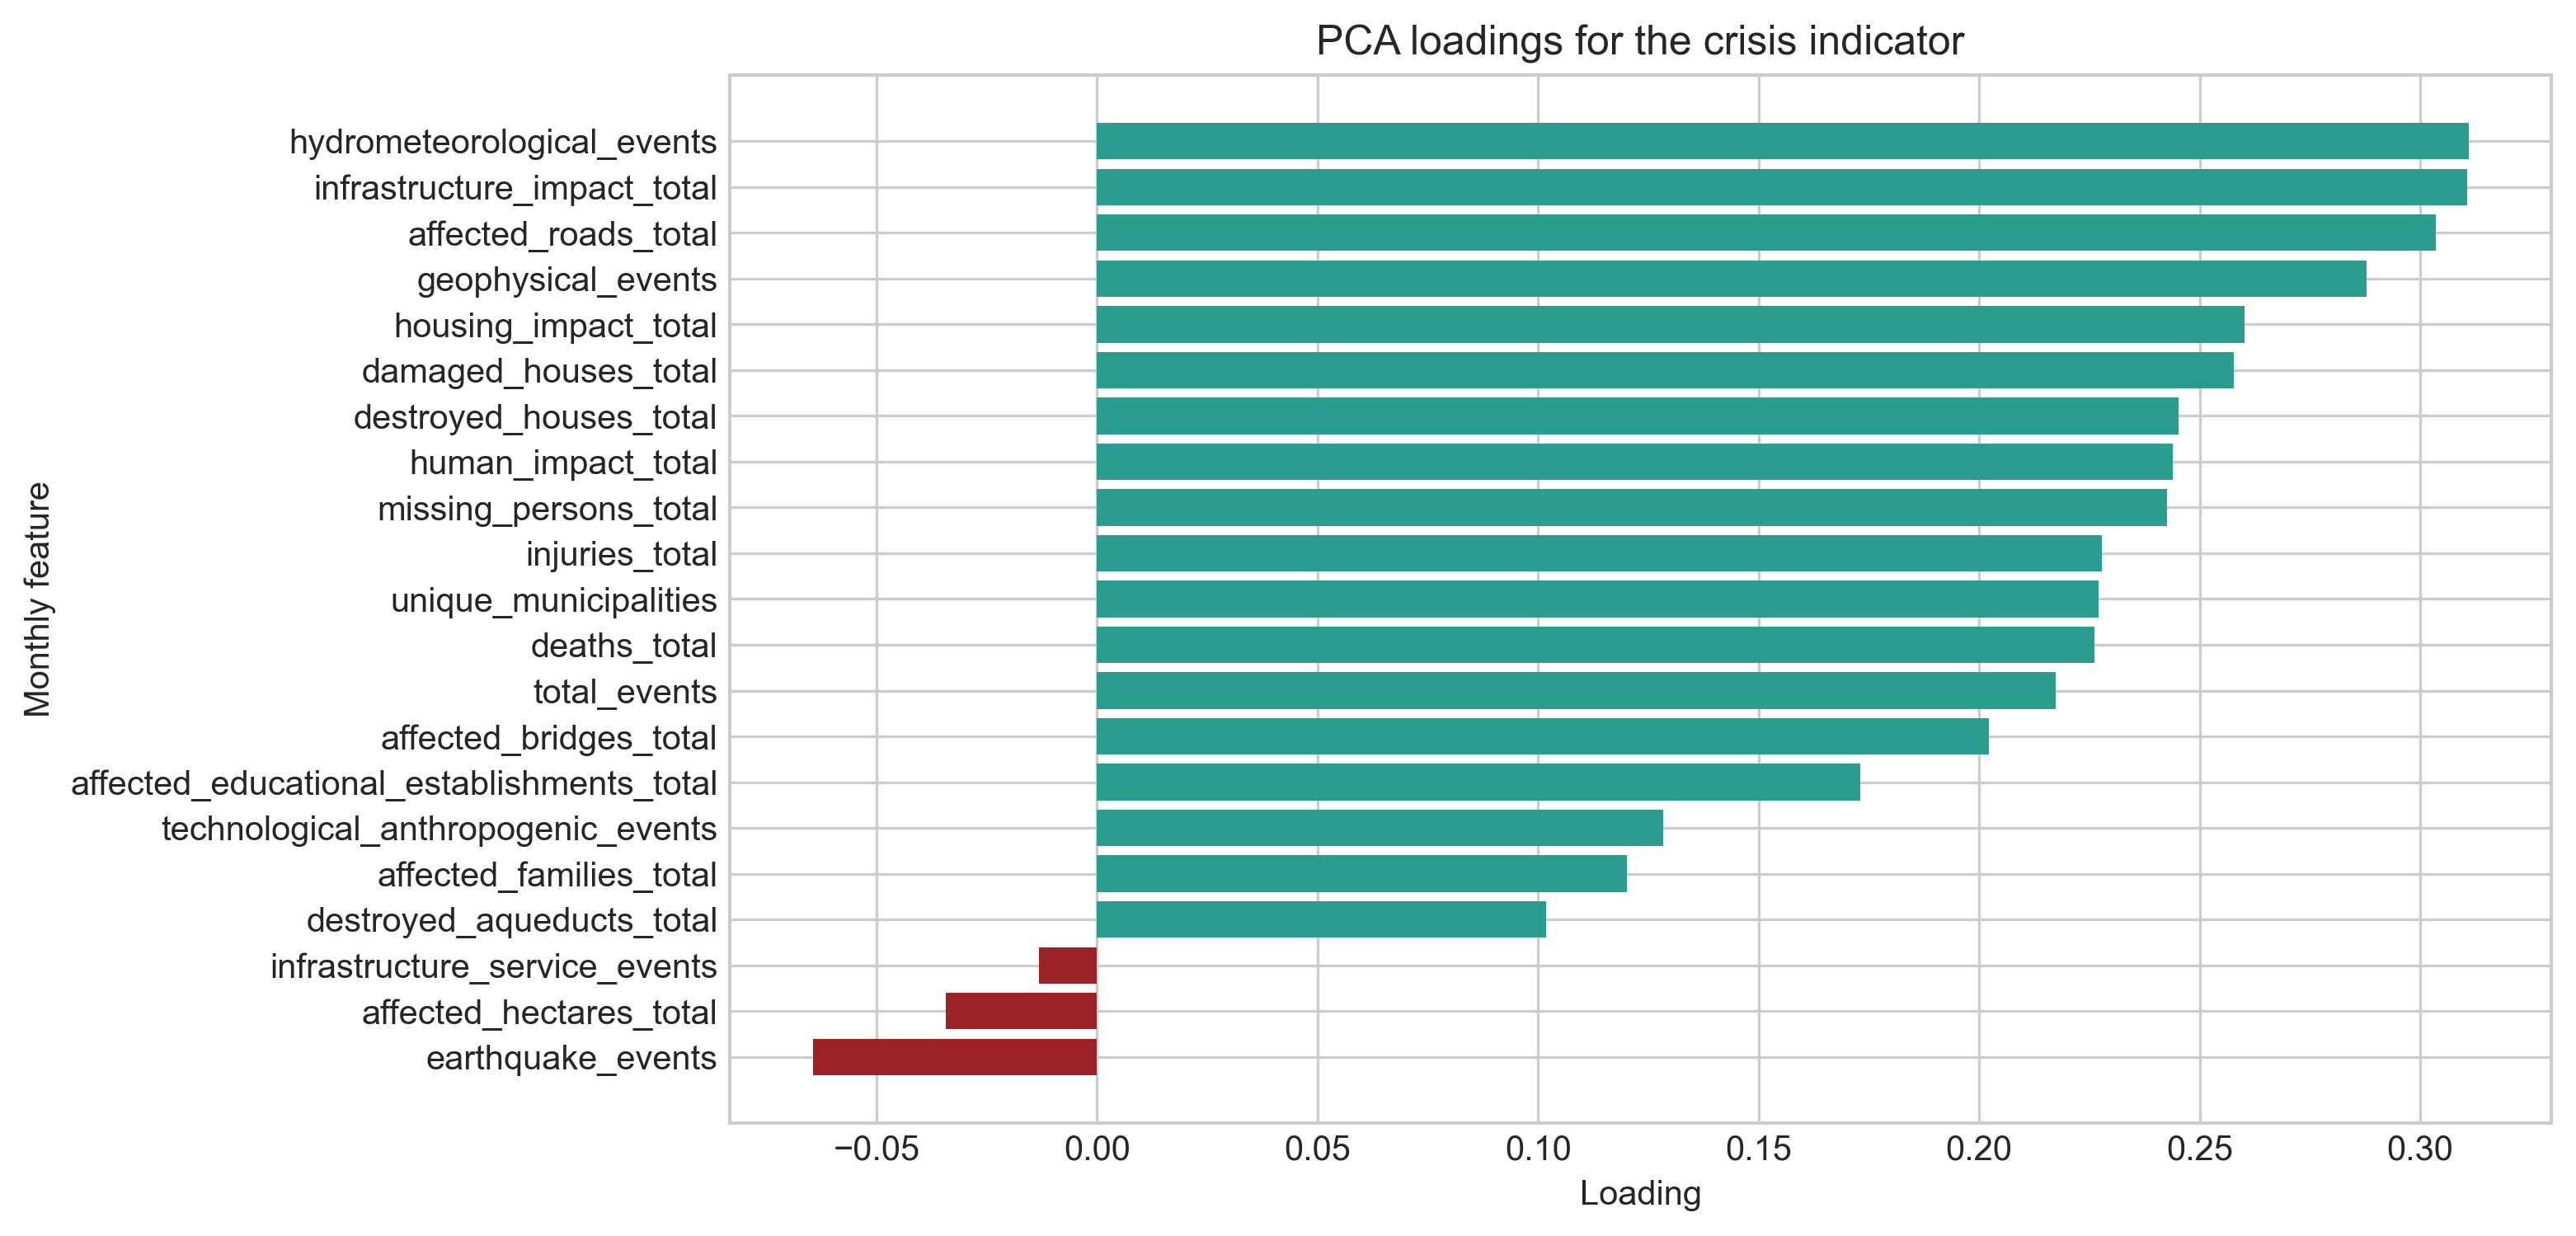
\includegraphics[width=0.70\textwidth]{figures/figure_pca_loadings.png}
\caption{Loadings for the first principal component of the multi-hazard disaster-pressure indicator. The figure is retained to document the composition of the synthetic robustness overlay used in the integrated article.}
\label{fig:supp_pca_loadings}
\end{figure}

\begin{table}[H]
\centering
\caption{Lag-specific pairwise Granger-causality $p$-values in the aligned core return system}
\label{tab:supp_granger}
\small
\begin{tabular}{p{4.6cm}rrrr}
\toprule
Direction & Lag 1 $p$ & Lag 2 $p$ & Lag 3 $p$ & Best lag ($p$) \\
\midrule
World cocoa $\rightarrow$ Colombian cocoa & 0.050 & 0.075 & 0.023 & 3 (0.023) \\
Colombian cocoa $\rightarrow$ World cocoa & 0.013 & 0.076 & 0.027 & 1 (0.013) \\
Colombian cocoa $\rightarrow$ EU chocolate & 0.979 & 0.801 & 0.871 & 2 (0.801) \\
EU chocolate $\rightarrow$ Colombian cocoa & 0.692 & 0.781 & 0.641 & 3 (0.641) \\
World cocoa $\rightarrow$ EU chocolate & 0.678 & 0.597 & 0.364 & 3 (0.364) \\
EU chocolate $\rightarrow$ World cocoa & 0.866 & 0.191 & 0.192 & 2 (0.191) \\
\bottomrule
\end{tabular}
\end{table}

\begin{table}[H]
\centering
\caption{Weather-extended domestic models retained from the first manuscript version}
\label{tab:supp_weather_models}
\small
\begin{tabular}{p{5.3cm}rrrr}
\toprule
Model component & Coefficient & Std. error & $p$-value & Adj. $R^2$ \\
\midrule
$\ln(P^{COL}_{t}) \leftarrow \ln(P^{WLD}_{t})$ & 0.977 & 0.037 & $<0.001$ & 0.966 \\
$\ln(P^{COL}_{t}) \leftarrow$ solar radiation$_t$ ($z$) & 0.028 & 0.016 & 0.075 & 0.966 \\
$\ln(P^{COL}_{t}) \leftarrow$ precipitation$_t$ ($z$) & 0.024 & 0.020 & 0.247 & 0.966 \\
$\ln(P^{COL}_{t}) \leftarrow$ max temperature$_t$ ($z$) & -0.009 & 0.019 & 0.627 & 0.966 \\
$\Delta \ln(P^{COL}_{t}) \leftarrow \Delta \ln(P^{WLD}_{t})$ & 0.773 & 0.157 & $<0.001$ & 0.595 \\
$\Delta \ln(P^{COL}_{t}) \leftarrow$ max temperature$_{t-1}$ ($z$) & 0.023 & 0.015 & 0.119 & 0.595 \\
$\Delta \ln(P^{COL}_{t}) \leftarrow$ precipitation$_{t-1}$ ($z$) & 0.003 & 0.010 & 0.725 & 0.595 \\
$\Delta \ln(P^{COL}_{t}) \leftarrow$ solar radiation$_{t-1}$ ($z$) & -0.008 & 0.008 & 0.330 & 0.595 \\
Domestic rolling volatility $\leftarrow$ world rolling volatility & 0.954 & 0.051 & $<0.001$ & 0.917 \\
Domestic rolling volatility $\leftarrow$ weather stress$_{t-1}$ & 0.013 & 0.012 & 0.253 & 0.917 \\
\bottomrule
\end{tabular}
\end{table}

\begin{table}[H]
\centering
\caption{Exploratory vulnerability indicators retained from the first manuscript version}
\label{tab:supp_vulnerability_defs}
\small
\begin{tabular}{p{3.0cm}p{8.2cm}rr}
\toprule
Indicator & Construction & Mean & Std. dev. \\
\midrule
Weather stress index & Mean absolute standardized anomaly across precipitation, solar radiation, and maximum temperature & 0.798 & 0.356 \\
Weather stress ($z$-score) & Standardized weather-stress index; positive values indicate above-average combined anomaly & 0.000 & 1.010 \\
Farmer exposure index & $z(\sigma^{COL}_t) + z(\widehat{m}_t) + \mathrm{WeatherStress}_t$ & 0.758 & 1.691 \\
Livelihood risk score & Farmer exposure index plus standardized world-cocoa volatility & 0.758 & 2.429 \\
\bottomrule
\end{tabular}
\end{table}

\begin{table}[H]
\centering
\caption{Disaster-indicator Granger-causality matrix retained from the disaster-extension manuscript}
\label{tab:supp_disaster_granger}
\small
\begin{tabular}{p{4.1cm}p{4.0cm}rrrr}
\toprule
Source & Target & Lag 1 $p$ & Lag 2 $p$ & Lag 3 $p$ & Lag 4 $p$ \\
\midrule
Disaster indicator & Colombian cocoa return & 0.876 & 0.987 & 0.983 & 0.967 \\
Disaster indicator & World cocoa return & 0.654 & 0.958 & 0.961 & 0.775 \\
Disaster indicator & FX return & 0.443 & 0.762 & 0.830 & 0.545 \\
Disaster indicator & Oil return & 0.383 & 0.575 & 0.677 & 0.627 \\
\bottomrule
\end{tabular}
\end{table}

\bibliographystyle{apalike}
\bibliography{references/cocoa_volatility}

\end{document}
